% ----- auto-generated from week_08/Week*.html via pandoc -----
\setchapterimage[6cm]{}
\setchapterpreamble[u]{\margintoc}
\chapter{Nonlinear Control Optimization for Robotic Systems}
\labch{week_08}

\section{Week 8: Nonlinear Control Optimization for Robotic Systems}\label{week-8-nonlinear-control-optimization-for-robotic-systems}}

From Pontryagin \& HJB to Optimized SMC, Adaptive, Robust, Backstepping, and NMPC

M.Sc. Control for Robots --- University of West London --- AY 2025--26\\
Week 8 of 12 (Control Theory Block) • Lecture + MATLAB Lab

\subsection{Section 1: Learning Outcomes}\label{section-1-learning-outcomes}}

By the end of this session, you will be able to:

\begin{itemize}
\tightlist
\item
  Explain why linear optimal control (LQR/LQG) is fundamentally insufficient for robotic systems whose dynamics are nonlinear
\item
  State the nonlinear optimal control problem and derive necessary conditions via Pontryagin\textquotesingle s Minimum Principle (PMP)
\item
  Formulate the nonlinear HJB equation and explain why direct solution is infeasible for robots
\item
  Describe direct transcription methods (single/multiple shooting, collocation) and apply iLQR / DDP and NMPC to a manipulator, mobile robot, and quadrotor
\item
  Pose the tuning of \textbf{sliding-mode}, \textbf{adaptive}, \textbf{robust}, \textbf{backstepping}, and \textbf{nonlinear MPC} controllers as constrained nonlinear optimization problems
\item
  Select appropriate decision variables, cost functionals, constraints, and solvers for each controller family
\item
  Interpret Pareto trade-offs (chattering vs. precision, speed vs. robustness, horizon vs. compute) through simulation
\end{itemize}

\subsection{Section 2: Session Roadmap}\label{section-2-session-roadmap}}

0:00--0:20

\paragraph{Part 1 --- Why linearization fails for robots}\label{part-1-why-linearization-fails-for-robots}}

Robot dynamics M(q)q̈ + C(q,q̇)q̇ + G(q) = τ are nonlinear globally. Jacobian linearization destroys Coriolis, gravity coupling, and singularity structure.

0:20--1:00

\paragraph{Part 2 --- Nonlinear optimization foundations}\label{part-2-nonlinear-optimization-foundations}}

Pontryagin minimum principle, nonlinear HJB, direct transcription, iLQR/DDP, nonlinear MPC.

1:00--2:30

\paragraph{Part 3 --- Optimization of each nonlinear controller}\label{part-3-optimization-of-each-nonlinear-controller}}

SMC, Adaptive, Robust, Backstepping, NMPC --- per-family decision variables, cost, constraints, and solvers, each demonstrated on manipulator / mobile / drone.

2:30--3:15

\paragraph{Part 4 --- Unified view and summary}\label{part-4-unified-view-and-summary}}

Common structure across families; LMI/SOS/Bayesian optimization/RL as cross-cutting tools; summary comparison.

3:15--4:00

\paragraph{Part 5 --- MATLAB lab}\label{part-5-matlab-lab}}

Run \texttt{run\_all.m} --- observe before/after cost for every controller on every robot. Modify cost weights and re-run.

\subsection{Section 3: Why Robots Demand Nonlinear Control Optimization}\label{section-3-why-robots-demand-nonlinear-control-optimization}}

\subsubsection{3.1 Robot dynamics are globally nonlinear}\label{robot-dynamics-are-globally-nonlinear}}

Every robotic system encountered in this course is governed by nonlinear ODEs:

\textbackslash{[}
\textbackslash underbrace\{M(q)\textbackslash,\textbackslash ddot\{q\} + C(q,\textbackslash dot\{q\})\textbackslash,\textbackslash dot\{q\} + G(q) = \textbackslash tau + d(t)\}\_\{\textbackslash text\{serial manipulator\}\}
\textbackslash{]}
\textbackslash{[}
\textbackslash underbrace\{\textbackslash dot\{p\}\_x = v\textbackslash cos\textbackslash theta,\textbackslash{} \textbackslash dot\{p\}\_y = v\textbackslash sin\textbackslash theta,\textbackslash{} \textbackslash dot\textbackslash theta = \textbackslash omega\}\_\{\textbackslash text\{unicycle mobile robot\}\}
\textbackslash{]}
\textbackslash{[}
\textbackslash underbrace\{m\textbackslash ddot\{\textbackslash mathbf\{p\}\} = R(\textbackslash Phi)\textbackslash mathbf\{F\}\_b - m\textbackslash mathbf\{g\},\textbackslash quad J\textbackslash dot\{\textbackslash boldsymbol\textbackslash omega\} + \textbackslash boldsymbol\textbackslash omega\textbackslash times J\textbackslash boldsymbol\textbackslash omega = \textbackslash boldsymbol\textbackslash tau\_b\}\_\{\textbackslash text\{quadrotor (rigid body)\}\}
\textbackslash{]}

\textbf{Variables used in the equations above:}

\begin{longtable}[]{@{}lll@{}}
\toprule\noalign{}
Symbol & Meaning & Typical units \\
\midrule\noalign{}
\endhead
\bottomrule\noalign{}
\endlastfoot
\textbackslash(q\textbackslash) & joint-angle (configuration) vector of the manipulator & rad \\
\textbackslash(\textbackslash dot q,\textbackslash{} \textbackslash ddot q\textbackslash) & joint velocity and acceleration & rad/s, rad/s² \\
\textbackslash(M(q)\textbackslash) & configuration-dependent inertia (mass) matrix; symmetric, positive-definite & kg·m² \\
\textbackslash(C(q,\textbackslash dot q)\textbackslash dot q\textbackslash) & Coriolis + centrifugal torque; quadratic in \textbackslash(\textbackslash dot q\textbackslash) & N·m \\
\textbackslash(G(q)\textbackslash) & gravity torque vector & N·m \\
\textbackslash(\textbackslash tau\textbackslash) & commanded joint torque (the control input \textbackslash(u\textbackslash)) & N·m \\
\textbackslash(d(t)\textbackslash) & lumped external / unmodelled disturbance torque & N·m \\
\textbackslash(p\_x,p\_y,\textbackslash theta\textbackslash) & mobile-robot pose: planar position and heading angle & m, m, rad \\
\textbackslash(v,\textbackslash omega\textbackslash) & mobile-robot linear and angular velocity commands & m/s, rad/s \\
\textbackslash(\textbackslash mathbf p\textbackslash) & quadrotor position vector in the inertial frame & m \\
\textbackslash(\textbackslash Phi\textbackslash) & quadrotor attitude (roll, pitch, yaw) & rad \\
\textbackslash(R(\textbackslash Phi)\textbackslash) & body-to-inertial rotation matrix, function of attitude & dimensionless, \textbackslash(3\textbackslash times 3\textbackslash) \\
\textbackslash(\textbackslash mathbf F\_b,\textbackslash boldsymbol\textbackslash tau\_b\textbackslash) & thrust vector and torque vector in the quadrotor body frame & N, N·m \\
\textbackslash(m\textbackslash) (quadrotor) & vehicle mass (scalar) & kg \\
\textbackslash(\textbackslash mathbf g\textbackslash) & gravity vector & m/s² \\
\textbackslash(J\textbackslash) (quadrotor) & body-frame inertia tensor & kg·m² \\
\textbackslash(\textbackslash boldsymbol\textbackslash omega\textbackslash) & body-frame angular velocity & rad/s \\
\end{longtable}

The nonlinearity is not incidental: it comes from \textbf{rotations} (trig terms in the unicycle and in \textbackslash(R(\textbackslash Phi)\textbackslash)), \textbf{Coriolis and centrifugal coupling} (\textbackslash(C(q,\textbackslash dot q)\textbackslash dot q\textbackslash) is quadratic in \textbackslash(\textbackslash dot q\textbackslash)), and \textbf{gravity} coupled through the kinematic chain (\textbackslash(G(q)\textbackslash) is a trigonometric function of \textbackslash(q\textbackslash)).

\subsubsection{3.2 Why Jacobian linearization is not enough}\label{why-jacobian-linearization-is-not-enough}}

The standard LQR recipe is: pick an equilibrium \textbackslash((x\^{}\textbackslash star, u\^{}\textbackslash star)\textbackslash), form \textbackslash(A = \textbackslash partial f/\textbackslash partial x\textbar\_\{x\^{}\textbackslash star\}\textbackslash), \textbackslash(B = \textbackslash partial f/\textbackslash partial u\textbar\_\{x\^{}\textbackslash star\}\textbackslash), solve the ARE. Three structural problems make this inadequate for robots:

\begin{itemize}
\tightlist
\item
  \textbf{Validity shrinks with aggressive motion.} The linear model is accurate only in a small neighbourhood of \textbackslash(x\^{}\textbackslash star\textbackslash). A manipulator swinging through \textbackslash(\textbackslash pi/2\textbackslash) is far outside any single linearization.
\item
  \textbf{Nonholonomic systems have no equilibrium at a generic state.} A mobile robot at pose \textbackslash((p\_x, p\_y, \textbackslash theta)\textbackslash) with \textbackslash(v = 0, \textbackslash omega = 0\textbackslash) is an equilibrium but the linearization is \emph{uncontrollable} there (Brockett\textquotesingle s theorem). LQR literally cannot stabilize heading.
\item
  \textbf{Parametric uncertainty cannot be addressed.} LQR presumes known \textbackslash((A,B)\textbackslash). Payload changes, friction, aero effects require adaptive / robust design --- none of which are optimal-control concepts in the linear sense.
\end{itemize}

\textbf{Take-home:} For robots, LQR is a \emph{local} stabilizer. Any optimization that meaningfully improves robot performance must work directly on the nonlinear dynamics, and must be applicable to the nonlinear controller families (SMC, adaptive, robust, backstepping, NMPC) you already know.

\subsubsection{3.3 Two meanings of ``control optimization''}\label{two-meanings-of-control-optimization}}

We unify two interpretations under one framework:

\begin{longtable}[]{@{}lll@{}}
\toprule\noalign{}
Meaning & What is optimized & Where it appears in this lecture \\
\midrule\noalign{}
\endhead
\bottomrule\noalign{}
\endlastfoot
\textbf{(A) Optimal trajectory} & The control signal \textbackslash(u(t)\textbackslash) itself --- infinite-dimensional decision variable & Section 4: PMP, HJB, iLQR/DDP, NMPC \\
\textbf{(B) Optimal controller tuning} & A finite set of gains / parameters \textbackslash(\textbackslash theta\textbackslash) inside a fixed control law \textbackslash(u = \textbackslash pi\_\textbackslash theta(x)\textbackslash) & Sections 5--9: SMC, Adaptive, Robust, Backstepping, NMPC tuning \\
\end{longtable}

Both are nonlinear optimization problems. The difference is only the dimension of the decision variable.

\subsection{Section 4: Foundations of Nonlinear Control Optimization}\label{section-4-foundations-of-nonlinear-control-optimization}}

\subsubsection{4.0 Notation used throughout Section 4}\label{notation-used-throughout-section-4}}

\begin{longtable}[]{@{}lll@{}}
\toprule\noalign{}
Symbol & Meaning & Dimensions \\
\midrule\noalign{}
\endhead
\bottomrule\noalign{}
\endlastfoot
\textbackslash(x,\textbackslash{} \textbackslash dot x\textbackslash) & state vector and its time derivative & \textbackslash(n\textbackslash times 1\textbackslash) \\
\textbackslash(u\textbackslash) & control / input vector & \textbackslash(m\textbackslash times 1\textbackslash) \\
\textbackslash(f(x,u)\textbackslash) & right-hand side of continuous-time dynamics \textbackslash(\textbackslash dot x = f(x,u)\textbackslash) & \textbackslash(n\textbackslash times 1\textbackslash) \\
\textbackslash(F(x,u)\textbackslash) & discrete-time one-step map: \textbackslash(x\_\{k+1\} = F(x\_k,u\_k)\textbackslash); typically \textbackslash(F = x + \textbackslash Delta t\textbackslash,f(x,u)\textbackslash) & \textbackslash(n\textbackslash times 1\textbackslash) \\
\textbackslash(\textbackslash Delta t\textbackslash) & sample time for discrete-time formulations & scalar \\
\textbackslash(N\textbackslash) & number of discrete time steps in the horizon & scalar \\
\textbackslash(T\textbackslash) & continuous horizon length, \textbackslash(T = N\textbackslash Delta t\textbackslash) & scalar \\
\textbackslash(L(x,u,t)\textbackslash) & instantaneous (stage) cost rate --- what you pay per unit time & scalar \\
\textbackslash(\textbackslash phi(x)\textbackslash) or \textbackslash(\textbackslash Phi(x)\textbackslash) & terminal cost --- what you pay at the end state \textbackslash(x(T)\textbackslash) or \textbackslash(x\_N\textbackslash) & scalar \\
\textbackslash(J\textbackslash) & total cost functional \textbackslash(\textbackslash phi + \textbackslash int L\textbackslash,dt\textbackslash) (or \textbackslash(\textbackslash sum L\_k + \textbackslash Phi\textbackslash)) & scalar \\
\textbackslash(g(x,u)\textbackslash) & inequality constraint function (e.g. torque limits, obstacles) & \textbackslash(p\textbackslash times 1\textbackslash) \\
\textbackslash(\textbackslash mathcal U\textbackslash) & admissible control set (e.g. box \textbackslash(\textbackslash\{u:\textbar u\textbar\textbackslash leq u\_\{\textbackslash max\}\textbackslash\}\textbackslash)) & subset of \textbackslash(\textbackslash mathbb R\^{}m\textbackslash) \\
\textbackslash(H(x,u,\textbackslash lambda,t)\textbackslash) & Hamiltonian: \textbackslash(L + \textbackslash lambda\^{}\{T\} f\textbackslash) & scalar \\
\textbackslash(\textbackslash lambda(t)\textbackslash) & \textbf{costate} (adjoint): shadow price of the constraint \textbackslash(\textbackslash dot x = f(x,u)\textbackslash); interpret as \textbackslash(\textbackslash partial V/\textbackslash partial x\textbackslash) & \textbackslash(n\textbackslash times 1\textbackslash) \\
\textbackslash(V(x,t)\textbackslash) or \textbackslash(V\_k(x)\textbackslash) & \textbf{value function}: minimum cost-to-go from state \textbackslash(x\textbackslash) at time \textbackslash(t\textbackslash) (or step \textbackslash(k\textbackslash)) to the horizon end & scalar \\
\textbackslash(\textbackslash nabla\_x V,\textbackslash{} V\_x\textbackslash) & gradient of the value function w.r.t. state & \textbackslash(n\textbackslash times 1\textbackslash) \\
\textbackslash(V\_\{xx\}\textbackslash) & Hessian of the value function w.r.t. state & \textbackslash(n\textbackslash times n\textbackslash) \\
superscript \textbackslash(\textbackslash star\textbackslash) & optimal quantity (e.g. \textbackslash(u\^{}\textbackslash star, x\^{}\textbackslash star, V\^{}\textbackslash star\textbackslash)) & --- \\
overbar (\textbackslash(\textbackslash bar x,\textbackslash bar u\textbackslash)) & nominal / current-iterate trajectory around which we expand & --- \\
\textbackslash(\textbackslash delta x,\textbackslash{} \textbackslash delta u\textbackslash) & perturbation from the nominal: \textbackslash(x = \textbackslash bar x + \textbackslash delta x\textbackslash) & \textbackslash(n,m\textbackslash times 1\textbackslash) \\
\end{longtable}

\subsubsection{4.1 The nonlinear optimal control problem}\label{the-nonlinear-optimal-control-problem}}

\textbackslash{[}
\textbackslash min\_\{u(\textbackslash cdot)\}\textbackslash{} J = \textbackslash phi\textbackslash bigl(x(T)\textbackslash bigr) + \textbackslash int\_0\^{}T L\textbackslash bigl(x(t), u(t), t\textbackslash bigr)\textbackslash,dt
\textbackslash{]}
subject to \textbackslash(\textbackslash dot x = f(x,u),\textbackslash{} x(0) = x\_0\textbackslash), and \textbackslash(g(x,u) \textbackslash leq 0\textbackslash)

Explicitly: we choose the entire control signal \textbackslash(u:{[}0,T{]}\textbackslash to\textbackslash mathbb R\^{}m\textbackslash) (an infinite-dimensional decision variable) to minimise the \emph{cost functional} \textbackslash(J\textbackslash) --- a real number equal to the terminal cost \textbackslash(\textbackslash phi\textbackslash) at the final state plus the time-integrated stage cost \textbackslash(L\textbackslash) along the whole trajectory. The trajectory \textbackslash(x(t)\textbackslash) is constrained to satisfy the nonlinear dynamics \textbackslash(\textbackslash dot x = f(x,u)\textbackslash) starting from a known initial state \textbackslash(x\_0\textbackslash), and the control and state may be additionally subject to path inequalities \textbackslash(g(x,u)\textbackslash le 0\textbackslash).

For robots, \textbackslash(f\textbackslash) is explicitly nonlinear (gravity, Coriolis, rotation trig). The stage cost \textbackslash(L\textbackslash) typically combines tracking error, control effort, and barrier-like constraint penalties. \textbackslash(\textbackslash phi\textbackslash) is the terminal cost.

\subsubsection{4.2 Pontryagin\textquotesingle s Minimum Principle (PMP)}\label{pontryagins-minimum-principle-pmp}}

PMP gives first-order necessary conditions for optimality. Introduce an auxiliary vector \textbackslash(\textbackslash lambda(t)\textbackslash in\textbackslash mathbb R\^{}n\textbackslash) --- the \textbf{costate} or adjoint --- which plays the role of a Lagrange multiplier for the dynamics constraint \textbackslash(\textbackslash dot x = f(x,u)\textbackslash). Define the \textbf{Hamiltonian}:

\textbackslash{[}
H(x, u, \textbackslash lambda, t) := \textbackslash underbrace\{L(x,u,t)\}\_\{\textbackslash text\{stage cost\}\} + \textbackslash underbrace\{\textbackslash lambda\^{}\{T\} f(x,u)\}\_\{\textbackslash substack\{\textbackslash text\{costate-weighted\} \textbackslash\textbackslash{} \textbackslash text\{dynamics\}\}\}
\textbackslash{]}

The Hamiltonian is a scalar that measures "instantaneous cost plus the marginal cost of moving the state in the direction \textbackslash(f\textbackslash)". An optimal trajectory \textbackslash((x\^{}\textbackslash star(t), u\^{}\textbackslash star(t))\textbackslash) with its associated costate \textbackslash(\textbackslash lambda\^{}\textbackslash star(t)\textbackslash) must satisfy the four conditions below. Each variable is defined explicitly:

\textbackslash{[}
\textbackslash begin\{array\}\{ll\}
\textbackslash dot x\^{}\textbackslash star(t) = \textbackslash partial H/\textbackslash partial\textbackslash lambda = f(x\^{}\textbackslash star, u\^{}\textbackslash star) \& \textbackslash text\{(state equation --- recovers the dynamics)\}\textbackslash\textbackslash{[}4pt{]}
\textbackslash dot\textbackslash lambda\^{}\textbackslash star(t) = -\textbackslash partial H/\textbackslash partial x\textbackslash big\textbar\_\textbackslash star \& \textbackslash text\{(costate equation, a.k.a.\textbackslash{} adjoint ODE)\}\textbackslash\textbackslash{[}4pt{]}
u\^{}\textbackslash star(t) = \textbackslash arg\textbackslash min\_\{u\textbackslash in\textbackslash mathcal U\} H(x\^{}\textbackslash star(t), u, \textbackslash lambda\^{}\textbackslash star(t), t) \& \textbackslash text\{(pointwise minimum principle)\}\textbackslash\textbackslash{[}4pt{]}
\textbackslash lambda\^{}\textbackslash star(T) = \textbackslash partial\textbackslash phi/\textbackslash partial x\textbackslash big\textbar\_\{x\^{}\textbackslash star(T)\} \& \textbackslash text\{(transversality / boundary condition at \} t=T)
\textbackslash end\{array\}
\textbackslash{]}

\textbf{What each variable does:}

\begin{itemize}
\tightlist
\item
  \textbackslash(\textbackslash lambda(t)\textbackslash in\textbackslash mathbb R\^{}n\textbackslash): costate --- informally, \textbackslash(\textbackslash lambda\_i\textbackslash) is the sensitivity of the optimal future cost to a perturbation in state component \textbackslash(x\_i\textbackslash).
\item
  \textbackslash(\textbackslash dot\textbackslash lambda = -\textbackslash partial H/\textbackslash partial x\textbackslash): costate evolves \emph{backward} in time; the minus sign makes the TPBVP a two-point boundary-value problem (state known at \textbackslash(t=0\textbackslash), costate known at \textbackslash(t=T\textbackslash)).
\item
  \textbackslash(u\^{}\textbackslash star = \textbackslash arg\textbackslash min\_\{u\textbackslash in\textbackslash mathcal U\} H\textbackslash): at each instant the optimal control minimises the Hamiltonian over the admissible set \textbackslash(\textbackslash mathcal U\textbackslash). If \textbackslash(\textbackslash mathcal U\textbackslash) is a box (torque limits) and \textbackslash(H\textbackslash) is linear in \textbackslash(u\textbackslash), the minimum is on the boundary --- \textbf{bang-bang}.
\item
  Transversality \textbackslash(\textbackslash lambda\^{}\textbackslash star(T) = \textbackslash phi\_x(x\^{}\textbackslash star(T))\textbackslash): at the final time the costate equals the gradient of the terminal cost, tying the two boundary conditions together.
\end{itemize}

PMP turns a functional optimisation into a two-point boundary-value problem (TPBVP) in \textbackslash((x,\textbackslash lambda)\textbackslash). Numerical TPBVP solvers (single/multiple shooting) construct this solution.

\subsubsection{4.3 Hamilton--Jacobi--Bellman (nonlinear)}\label{hamiltonjacobibellman-nonlinear}}

Where PMP gives necessary conditions for \emph{one} trajectory, HJB characterises the \textbf{value function} \textbackslash(V\^{}\textbackslash star(x,t)\textbackslash) over the whole state space. The value function is defined as the minimum cost-to-go:

\textbackslash{[}
V\^{}\textbackslash star(x, t) := \textbackslash min\_\{u(\textbackslash cdot)\} \textbackslash{} \textbackslash Bigl\textbackslash\{ \textbackslash phi\textbackslash bigl(x(T)\textbackslash bigr) + \textbackslash int\_t\^{}T L\textbackslash bigl(x(\textbackslash tau), u(\textbackslash tau), \textbackslash tau\textbackslash bigr)\textbackslash,d\textbackslash tau\textbackslash{} \textbackslash Big\textbar\textbackslash{} x(t) = x \textbackslash Bigr\textbackslash\}
\textbackslash{]}

i.e.\textbackslash{} "if I am currently at state \textbackslash(x\textbackslash) at time \textbackslash(t\textbackslash), what is the smallest remaining cost I can achieve by optimal play?" The Bellman principle of optimality implies that \textbackslash(V\^{}\textbackslash star\textbackslash) satisfies the HJB partial differential equation:

\textbackslash{[}
-\textbackslash frac\{\textbackslash partial V\^{}\textbackslash star\}\{\textbackslash partial t\}(x,t) \textbackslash{} =\textbackslash{} \textbackslash min\_\{u\textbackslash in\textbackslash mathcal U\}\textbackslash{} \textbackslash Bigl\textbackslash\{\textbackslash{} L(x,u,t)\textbackslash{} +\textbackslash{} \textbackslash underbrace\{(\textbackslash nabla\_x V\^{}\textbackslash star)\^{}\{T\}\}\_\{\textbackslash text\{value gradient\}\}\textbackslash,f(x,u)\textbackslash{} \textbackslash Bigr\textbackslash\},\textbackslash qquad V\^{}\textbackslash star(x,T) = \textbackslash phi(x)
\textbackslash{]}

\textbf{What each variable does:}

\begin{itemize}
\tightlist
\item
  \textbackslash(V\^{}\textbackslash star:\textbackslash mathbb R\^{}n\textbackslash times{[}0,T{]}\textbackslash to\textbackslash mathbb R\textbackslash): the scalar "cost-to-go" function, defined on the whole state space.
\item
  \textbackslash(\textbackslash partial V\^{}\textbackslash star/\textbackslash partial t\textbackslash): rate of change of the value as time moves forward at fixed state.
\item
  \textbackslash(\textbackslash nabla\_x V\^{}\textbackslash star \textbackslash in\textbackslash mathbb R\^{}n\textbackslash): the spatial gradient --- exactly the costate \textbackslash(\textbackslash lambda\textbackslash) from PMP, evaluated at \textbackslash((x,t)\textbackslash). This is the formal link: PMP lives on \emph{one} trajectory, HJB gives the gradient of the value over \emph{all} states.
\item
  The minimisation over \textbackslash(u\textbackslash) is pointwise at each \textbackslash((x,t)\textbackslash) (same operation as in PMP).
\item
  Terminal condition \textbackslash(V\^{}\textbackslash star(x,T) = \textbackslash phi(x)\textbackslash): at the end of the horizon the value equals the terminal cost.
\end{itemize}

HJB gives the optimal value function \emph{globally}, but direct solution is impractical for \textbackslash(\textbackslash dim x \textbackslash ge 4\textbackslash) (curse of dimensionality) --- grid-based methods scale as \textbackslash(O(N\_\{\textbackslash text\{grid\}\}\^{}n)\textbackslash). HJB remains the theoretical yardstick against which PMP and direct methods are justified.

\subsubsection{4.4 Direct methods: shooting and collocation}\label{direct-methods-shooting-and-collocation}}

Discretize time into \textbackslash(N\textbackslash) knots, turn the infinite-dimensional problem into a finite nonlinear program (NLP).

\begin{longtable}[]{@{}llll@{}}
\toprule\noalign{}
Method & Decision variables & Pros & Cons \\
\midrule\noalign{}
\endhead
\bottomrule\noalign{}
\endlastfoot
Single shooting & \textbackslash((u\_0,\textbackslash ldots,u\_\{N-1\})\textbackslash); states propagated & Few variables & Highly nonlinear NLP, sensitive to \textbackslash(u\_0\textbackslash) \\
Multiple shooting & States at knots + controls; defect constraints & Better conditioning, parallel integration & More variables \& equality constraints \\
Direct collocation & States \& controls at all knots; dynamics as algebraic constraint & Sparse structure, handles unstable dynamics & High-dimensional NLP; needs sparse SQP/IPM solver \\
\end{longtable}

\subsubsection{4.5 iLQR and DDP --- the robot trajectory optimizer of choice}\label{ilqr-and-ddp-the-robot-trajectory-optimizer-of-choice}}

\textbf{Iterative LQR (iLQR)} linearises the dynamics \textbackslash(f\textbackslash) around a \emph{nominal} (current-iterate) trajectory, quadratises the cost around the same nominal, solves the resulting time-varying LQR problem exactly, and updates the trajectory. \textbf{Differential Dynamic Programming (DDP)} is the second-order variant that also keeps the Hessians of \textbackslash(f\textbackslash). Both converge \emph{locally quadratically} --- one iteration is one Newton step on the Bellman recursion.

\paragraph{Symbols used in the iLQR recursion}\label{symbols-used-in-the-ilqr-recursion}}

\begin{longtable}[]{@{}lll@{}}
\toprule\noalign{}
Symbol & Meaning & Dimensions \\
\midrule\noalign{}
\endhead
\bottomrule\noalign{}
\endlastfoot
\textbackslash(k\textbackslash) & discrete time-step index, \textbackslash(k = 0,1,\textbackslash ldots,N\textbackslash) & integer \\
\textbackslash(\textbackslash bar x\_k,\textbackslash{} \textbackslash bar u\_k\textbackslash) & nominal state / control at step \textbackslash(k\textbackslash) (current iterate; iLQR improves this each pass) & \textbackslash(n,\textbackslash{} m\textbackslash) \\
\textbackslash(\textbackslash delta x\_k\textbackslash) & state perturbation from the nominal: \textbackslash(x\_k = \textbackslash bar x\_k + \textbackslash delta x\_k\textbackslash) & \textbackslash(n\textbackslash times 1\textbackslash) \\
\textbackslash(\textbackslash delta u\_k\textbackslash) & control perturbation: \textbackslash(u\_k = \textbackslash bar u\_k + \textbackslash delta u\_k\textbackslash) & \textbackslash(m\textbackslash times 1\textbackslash) \\
\textbackslash(A\_k\textbackslash) & state Jacobian \textbackslash(\textbackslash partial F/\textbackslash partial x\textbackslash) at \textbackslash((\textbackslash bar x\_k,\textbackslash bar u\_k)\textbackslash) --- how a \textbackslash(\textbackslash delta x\textbackslash) propagates one step & \textbackslash(n\textbackslash times n\textbackslash) \\
\textbackslash(B\_k\textbackslash) & control Jacobian \textbackslash(\textbackslash partial F/\textbackslash partial u\textbackslash) at \textbackslash((\textbackslash bar x\_k,\textbackslash bar u\_k)\textbackslash) --- how \textbackslash(\textbackslash delta u\textbackslash) enters the next state & \textbackslash(n\textbackslash times m\textbackslash) \\
\textbackslash(L\_k\textbackslash) & stage cost evaluated at \textbackslash((\textbackslash bar x\_k,\textbackslash bar u\_k)\textbackslash) & scalar \\
\textbackslash(L\_\{x,k\},L\_\{u,k\}\textbackslash) & gradients of the stage cost w.r.t. \textbackslash(x\textbackslash) and \textbackslash(u\textbackslash) & \textbackslash(n,\textbackslash{} m\textbackslash) \\
\textbackslash(L\_\{xx,k\},L\_\{uu,k\},L\_\{ux,k\}\textbackslash) & Hessians: pure-state, pure-control, and cross-second-derivative of stage cost & \textbackslash(n\{\textbackslash times\}n,\textbackslash{} m\{\textbackslash times\}m,\textbackslash{} m\{\textbackslash times\}n\textbackslash) \\
\textbackslash(V\_k(x)\textbackslash) & value function at step \textbackslash(k\textbackslash) (min cost-to-go) & scalar \\
\textbackslash(V\_\{x,k\},\textbackslash{} V\_\{xx,k\}\textbackslash) & value-function gradient and Hessian at \textbackslash((\textbackslash bar x\_k)\textbackslash) & \textbackslash(n,\textbackslash{} n\{\textbackslash times\}n\textbackslash) \\
\textbackslash(\textbackslash Phi(x)\textbackslash) & terminal cost; \textbackslash(V\_N(x) = \textbackslash Phi(x)\textbackslash) & scalar \\
\textbackslash(Q\_k(x,u)\textbackslash) & stage+future: \textbackslash(Q\_k = L(x,u) + V\_\{k+1\}(F(x,u))\textbackslash). Its minimiser over \textbackslash(u\textbackslash) is \textbackslash(V\_k\textbackslash). & scalar \\
\textbackslash(Q\_\{u,k\}\textbackslash) & gradient of \textbackslash(Q\_k\textbackslash) w.r.t. \textbackslash(u\textbackslash): \textbackslash(L\_\{u,k\} + B\_k\^{}\{T\} V\_\{x,k+1\}\textbackslash) & \textbackslash(m\textbackslash times 1\textbackslash) \\
\textbackslash(Q\_\{uu,k\}\textbackslash) & Hessian of \textbackslash(Q\_k\textbackslash) w.r.t. \textbackslash(u\textbackslash): \textbackslash(L\_\{uu,k\} + B\_k\^{}\{T\} V\_\{xx,k+1\} B\_k\textbackslash) & \textbackslash(m\textbackslash times m\textbackslash) \\
\textbackslash(Q\_\{ux,k\}\textbackslash) & cross Hessian of \textbackslash(Q\_k\textbackslash): \textbackslash(L\_\{ux,k\} + B\_k\^{}\{T\} V\_\{xx,k+1\} A\_k\textbackslash) & \textbackslash(m\textbackslash times n\textbackslash) \\
\textbackslash(Q\_\{x,k\}\textbackslash) & gradient of \textbackslash(Q\_k\textbackslash) w.r.t. \textbackslash(x\textbackslash): \textbackslash(L\_\{x,k\} + A\_k\^{}\{T\} V\_\{x,k+1\}\textbackslash) & \textbackslash(n\textbackslash times 1\textbackslash) \\
\textbackslash(Q\_\{xx,k\}\textbackslash) & Hessian of \textbackslash(Q\_k\textbackslash) w.r.t. \textbackslash(x\textbackslash): \textbackslash(L\_\{xx,k\} + A\_k\^{}\{T\} V\_\{xx,k+1\} A\_k\textbackslash) & \textbackslash(n\textbackslash times n\textbackslash) \\
\textbackslash(k\_k\textbackslash) & \textbf{feedforward correction}: \textbackslash(-Q\_\{uu,k\}\^{}\{-1\} Q\_\{u,k\}\textbackslash) --- how much to push \textbackslash(\textbackslash bar u\_k\textbackslash) in the best direction & \textbackslash(m\textbackslash times 1\textbackslash) \\
\textbackslash(K\_k\textbackslash) & \textbf{time-varying feedback gain}: \textbackslash(-Q\_\{uu,k\}\^{}\{-1\} Q\_\{ux,k\}\textbackslash) --- LQR-like feedback on the state perturbation & \textbackslash(m\textbackslash times n\textbackslash) \\
\textbackslash(\textbackslash alpha\textbackslash) & line-search step size, \textbackslash(\textbackslash alpha\textbackslash in(0,1{]}\textbackslash), reduced on forward-pass failure & scalar \\
\textbackslash(\textbackslash mu\textbackslash) & Levenberg--Marquardt regularisation added to \textbackslash(Q\_\{uu\}\textbackslash) for numerical robustness & scalar \\
\end{longtable}

\paragraph{Core iLQR recursion --- with full symbol definitions}\label{core-ilqr-recursion-with-full-symbol-definitions}}

\textbf{Setup.} We want to minimise \textbackslash(J = \textbackslash sum\_\{k=0\}\^{}\{N-1\} L(x\_k,u\_k) + \textbackslash Phi(x\_N)\textbackslash) subject to \textbackslash(x\_\{k+1\} = F(x\_k, u\_k)\textbackslash) starting from \textbackslash(x\_0\textbackslash). Assume we have a current-iterate \emph{nominal} trajectory \textbackslash(\textbackslash\{\textbackslash bar x\_k,\textbackslash bar u\_k\textbackslash\}\_\{k=0\}\^{}\{N\}\textbackslash). Let \textbackslash(x = \textbackslash bar x + \textbackslash delta x\textbackslash), \textbackslash(u = \textbackslash bar u + \textbackslash delta u\textbackslash) denote the unknown corrections.

\textbf{Step 1 --- Linearise the dynamics} at each nominal point \textbackslash((\textbackslash bar x\_k,\textbackslash bar u\_k)\textbackslash):

\textbackslash{[}
\textbackslash delta x\_\{k+1\} \textbackslash approx A\_k\textbackslash,\textbackslash delta x\_k + B\_k\textbackslash,\textbackslash delta u\_k,\textbackslash qquad A\_k := \textbackslash left.\textbackslash dfrac\{\textbackslash partial F\}\{\textbackslash partial x\}\textbackslash right\textbar\_\textbackslash star,\textbackslash{} B\_k := \textbackslash left.\textbackslash dfrac\{\textbackslash partial F\}\{\textbackslash partial u\}\textbackslash right\textbar\_\textbackslash star
\textbackslash{]}

\textbackslash(A\_k\textbackslash) is the \textbackslash(n\textbackslash times n\textbackslash) one-step state-transition matrix of the linearised dynamics; \textbackslash(B\_k\textbackslash) is the \textbackslash(n\textbackslash times m\textbackslash) input matrix. Both are computed by finite differences in code.

\textbf{Step 2 --- Quadratise the stage cost.} To second order,

\textbackslash{[}
L(\textbackslash bar x + \textbackslash delta x, \textbackslash bar u + \textbackslash delta u) \textbackslash approx L\_k + L\_\{x,k\}\^{}\{T\}\textbackslash delta x + L\_\{u,k\}\^{}\{T\}\textbackslash delta u + \textbackslash tfrac12\textbackslash!\textbackslash begin\{bmatrix\}\textbackslash delta x \textbackslash\textbackslash{} \textbackslash delta u\textbackslash end\{bmatrix\}\^{}\{T\}\textbackslash!\textbackslash!\textbackslash begin\{bmatrix\} L\_\{xx,k\} \& L\_\{xu,k\}\textbackslash\textbackslash{} L\_\{ux,k\} \& L\_\{uu,k\}\textbackslash end\{bmatrix\}\textbackslash!\textbackslash!\textbackslash begin\{bmatrix\}\textbackslash delta x\textbackslash\textbackslash{} \textbackslash delta u\textbackslash end\{bmatrix\}
\textbackslash{]}

where \textbackslash(L\_\{x,k\},L\_\{u,k\}\textbackslash) are gradients (of length \textbackslash(n,m\textbackslash) respectively) and \textbackslash(L\_\{xx,k\},L\_\{uu,k\},L\_\{ux,k\}\textbackslash) are Hessians/cross-Hessians of the stage cost at the nominal.

\textbf{Step 3 --- Define the \textbackslash(Q\textbackslash)-function.} Combining the stage cost with a quadratic model of the future-value function \textbackslash(V\_\{k+1\}\textbackslash):

\textbackslash{[}
Q\_k(\textbackslash delta x,\textbackslash delta u) \textbackslash equiv L(\textbackslash bar x+\textbackslash delta x,\textbackslash bar u+\textbackslash delta u)\textbackslash{} +\textbackslash{} V\_\{k+1\}(\textbackslash bar x\_\{k+1\} + A\_k\textbackslash delta x + B\_k\textbackslash delta u)
\textbackslash{]}

Expanding each piece to second order and collecting by power of \textbackslash(\textbackslash delta x, \textbackslash delta u\textbackslash) yields the five \textbackslash(Q\textbackslash)-blocks (each defined above):

\textbackslash{[}
Q\_\{x,k\} = L\_\{x,k\} + A\_k\^{}\{T\} V\_\{x,k+1\},\textbackslash qquad Q\_\{u,k\} = L\_\{u,k\} + B\_k\^{}\{T\} V\_\{x,k+1\}
\textbackslash{]}
\textbackslash{[}
Q\_\{xx,k\} = L\_\{xx,k\} + A\_k\^{}\{T\} V\_\{xx,k+1\} A\_k,\textbackslash quad Q\_\{uu,k\} = L\_\{uu,k\} + B\_k\^{}\{T\} V\_\{xx,k+1\} B\_k,\textbackslash quad Q\_\{ux,k\} = L\_\{ux,k\} + B\_k\^{}\{T\} V\_\{xx,k+1\} A\_k
\textbackslash{]}

\textbf{Step 4 --- Minimise \textbackslash(Q\_k\textbackslash) over \textbackslash(\textbackslash delta u\textbackslash) (closed-form).} Since \textbackslash(Q\_k\textbackslash) is quadratic in \textbackslash(\textbackslash delta u\textbackslash), the stationary condition \textbackslash(\textbackslash partial Q\_k/\textbackslash partial(\textbackslash delta u) = 0\textbackslash) reads

\textbackslash{[}
Q\_\{u,k\} + Q\_\{uu,k\}\textbackslash,\textbackslash delta u + Q\_\{ux,k\}\textbackslash,\textbackslash delta x = 0
\textbackslash{]}

Solving:

\textbackslash{[}
\textbackslash boxed\{\textbackslash{} \textbackslash delta u\_k\^{}\textbackslash star(\textbackslash delta x) = k\_k + K\_k\textbackslash,\textbackslash delta x\textbackslash{} \},\textbackslash qquad k\_k = -Q\_\{uu,k\}\^{}\{-1\} Q\_\{u,k\},\textbackslash quad K\_k = -Q\_\{uu,k\}\^{}\{-1\} Q\_\{ux,k\}
\textbackslash{]}

\textbackslash(k\_k \textbackslash in \textbackslash mathbb R\^{}m\textbackslash) is the \textbf{feedforward correction} (independent of the current state perturbation --- how much to push \textbackslash(\textbackslash bar u\_k\textbackslash) in the best direction). \textbackslash(K\_k\textbackslash in\textbackslash mathbb R\^{}\{m\textbackslash times n\}\textbackslash) is the \textbf{time-varying feedback gain} (LQR-style gain on \textbackslash(\textbackslash delta x\_k\textbackslash)).

\textbf{Step 5 --- Propagate the value function backward.} Substituting \textbackslash(\textbackslash delta u = k\_k + K\_k\textbackslash delta x\textbackslash) back into \textbackslash(Q\_k\textbackslash) gives a new quadratic in \textbackslash(\textbackslash delta x\textbackslash):

\textbackslash{[}
V\_\{x,k\} = Q\_\{x,k\} - K\_k\^{}\{T\} Q\_\{uu,k\}\textbackslash,k\_k,\textbackslash qquad V\_\{xx,k\} = Q\_\{xx,k\} - K\_k\^{}\{T\} Q\_\{uu,k\}\textbackslash,K\_k
\textbackslash{]}

Initialise at the horizon with \textbackslash(V\_\{x,N\} = \textbackslash Phi\_x(\textbackslash bar x\_N)\textbackslash), \textbackslash(V\_\{xx,N\} = \textbackslash Phi\_\{xx\}(\textbackslash bar x\_N)\textbackslash). Sweep \textbackslash(k = N\textbackslash!-\textbackslash!1,\textbackslash ldots,0\textbackslash).

\textbf{Step 6 --- Forward pass with line search.} With all \textbackslash(\textbackslash\{k\_k, K\_k\textbackslash\}\textbackslash) stored from the backward sweep, roll out a new trajectory starting from \textbackslash(\textbackslash delta x\_0 = 0\textbackslash):

\textbackslash{[}
\textbackslash delta u\_k = \textbackslash alpha\textbackslash,k\_k + K\_k\textbackslash,\textbackslash delta x\_k,\textbackslash quad u\_k\^{}\{\textbackslash text\{new\}\} = \textbackslash bar u\_k + \textbackslash delta u\_k,\textbackslash quad x\_\{k+1\}\^{}\{\textbackslash text\{new\}\} = F(x\_k\^{}\{\textbackslash text\{new\}\}, u\_k\^{}\{\textbackslash text\{new\}\})
\textbackslash{]}

The step size \textbackslash(\textbackslash alpha\textbackslash in(0,1{]}\textbackslash) is reduced (\textbackslash(\textbackslash alpha\textbackslash leftarrow \textbackslash alpha/2\textbackslash)) until the new cost \textbackslash(J\^{}\{\textbackslash text\{new\}\}

\textbf{Step 7 --- Regularise if \textbackslash(Q\_\{uu\}\textbackslash) is ill-conditioned.} Replace \textbackslash(Q\_\{uu,k\}\textbackslash) by \textbackslash(Q\_\{uu,k\} + \textbackslash mu I\_m\textbackslash) with \textbackslash(\textbackslash mu\textbackslash ge 0\textbackslash) increased on backward-pass Cholesky failure or forward-pass line-search failure. This is the Levenberg--Marquardt trust-region logic in the code.

\textbf{Output.} On convergence iLQR returns:

\begin{itemize}
\tightlist
\item
  A locally optimal trajectory \textbackslash(\textbackslash\{x\_k\^{}\textbackslash star, u\_k\^{}\textbackslash star\textbackslash\}\textbackslash) (the "open-loop" command);
\item
  A time-varying feedback policy \textbackslash(u\_k = u\_k\^{}\textbackslash star + K\_k(x - x\_k\^{}\textbackslash star)\textbackslash) valid in a neighbourhood of the trajectory --- this is the \emph{local} feedback that makes iLQR more robust than pure open-loop planning.
\end{itemize}

\subsubsection{4.6 Nonlinear MPC (NMPC)}\label{nonlinear-mpc-nmpc}}

NMPC wraps a trajectory optimiser (§4.5) in a \emph{receding-horizon} loop. At every sample instant \textbackslash(t\_k\textbackslash):

\begin{enumerate}
\tightlist
\item
  Measure the current state \textbackslash(x\_k\textbackslash).
\item
  Solve the finite-horizon OCP of §4.1 starting from \textbackslash(x\_0 := x\_k\textbackslash), over a fixed prediction horizon of \textbackslash(N\textbackslash) steps (duration \textbackslash(T = N\textbackslash Delta t\textbackslash)). This returns an optimal sequence \textbackslash(\textbackslash\{u\_0\^{}\textbackslash star, u\_1\^{}\textbackslash star, \textbackslash ldots, u\_\{N-1\}\^{}\textbackslash star\textbackslash\}\textbackslash).
\item
  Apply \emph{only the first} control \textbackslash(u\_0\^{}\textbackslash star\textbackslash) to the physical plant for one sample time \textbackslash(\textbackslash Delta t\textbackslash).
\item
  Shift the remaining solution \textbackslash((u\_1\^{}\textbackslash star,\textbackslash ldots,u\_\{N-1\}\^{}\textbackslash star,u\_\{N-1\}\^{}\textbackslash star)\textbackslash) and use it as the warm-start for step (2) at the next sample.
\end{enumerate}

\textbf{Key symbols:} \textbackslash(N\textbackslash) = horizon length (number of prediction steps); \textbackslash(\textbackslash Delta t\textbackslash) = sample time; \textbackslash(T = N\textbackslash Delta t\textbackslash) = prediction-window duration. The controller is therefore parameterised by \textbackslash((N, \textbackslash Delta t, Q, R, P, \textbackslash mathcal X\_f)\textbackslash) where \textbackslash(Q, R\textbackslash) are stage-cost weighting matrices, \textbackslash(P\textbackslash) the terminal-cost weighting, and \textbackslash(\textbackslash mathcal X\_f\textbackslash) the terminal invariance set.

Real-time implementations use \emph{warm-starting} (the previous solution shifted by one step is the initial guess for the new NLP) and \emph{SQP real-time iteration} (one Sequential Quadratic Programming step per sample, rather than iterating to full convergence). The dominant open-source libraries (ACADO, CasADi/Ipopt, acados) all implement variants of this loop.

\textbf{Key insight:} iLQR is a one-shot trajectory optimizer; NMPC is a receding-horizon feedback controller that \emph{uses} trajectory optimization at every sample. For robots with disturbances and uncertain initial conditions, NMPC is the preferred deployment form.

\subsection{Section 5: Optimization of Sliding Mode Control}\label{section-5-optimization-of-sliding-mode-control}}

\subsubsection{5.1 Free parameters of SMC}\label{free-parameters-of-smc}}

Recall the SMC law \textbackslash(\textbackslash tau = \textbackslash tau\_\{eq\} + \textbackslash tau\_\{sw\}\textbackslash) with \textbackslash(\textbackslash tau\_\{sw\} = -\textbackslash eta\textbackslash,\textbackslash mathrm\{sat\}(s/\textbackslash phi)\textbackslash), \textbackslash(s = \textbackslash dot e + \textbackslash lambda e\textbackslash). The controller is fully specified by three parameters per joint:

\begin{itemize}
\tightlist
\item
  \textbackslash(\textbackslash lambda\textbackslash) --- sliding surface slope: sets the reaching-phase-free convergence rate
\item
  \textbackslash(\textbackslash phi\textbackslash) --- boundary-layer width: chattering vs. steady-state error
\item
  \textbackslash(\textbackslash eta\textbackslash) --- switching gain: robustness margin vs. disturbance bound \textbackslash(D\textbackslash)
\end{itemize}

\subsubsection{5.2 Optimization formulation}\label{optimization-formulation}}

\textbackslash{[}
\textbackslash min\_\{\textbackslash lambda,\textbackslash phi,\textbackslash eta\} \textbackslash quad w\_e\textbackslash!\textbackslash!\textbackslash int\_0\^{}T\textbackslash!\textbackslash! \textbackslash\textbar e\textbackslash\textbar\^{}2\textbackslash,dt + w\_u\textbackslash!\textbackslash!\textbackslash int\_0\^{}T\textbackslash!\textbackslash! \textbackslash\textbar\textbackslash tau\textbackslash\textbar\^{}2\textbackslash,dt + w\_c\textbackslash!\textbackslash!\textbackslash int\_0\^{}T\textbackslash!\textbackslash! \textbackslash\textbar\textbackslash dot\textbackslash tau\textbackslash\textbar\textbackslash,dt
\textbackslash{]}
s.t. \textbackslash(\textbackslash eta \textgreater{} D\textbackslash) (reaching condition),\textbackslash; \textbackslash(\textbackslash lambda \textgreater{} 0\textbackslash),\textbackslash; \textbackslash(\textbackslash phi \textgreater{} 0\textbackslash),\textbackslash; \textbackslash(\textbar\textbackslash tau\textbar\textbackslash leq \textbackslash tau\_\{\textbackslash max\}\textbackslash)

The third term is a \textbf{chatter metric} (total variation of the control). This formalizes the Pareto trade-off studied in the Week 7 exam question.

\subsubsection{\texorpdfstring{5.3 LMI-based sliding-surface design --- \emph{full derivation}}{5.3 LMI-based sliding-surface design --- full derivation}}\label{lmi-based-sliding-surface-design-full-derivation}}

\paragraph{Step 1. Linearization of the robot around the operating point}\label{step-1.-linearization-of-the-robot-around-the-operating-point}}

Start from the nonlinear robot dynamics \textbackslash(\textbackslash dot x = f(x,u)\textbackslash) with \textbackslash(x = {[}q;\textbackslash dot q{]} \textbackslash in \textbackslash mathbb R\^{}n\textbackslash), \textbackslash(u = \textbackslash tau \textbackslash in \textbackslash mathbb R\^{}m\textbackslash). The Jacobian linearization at the operating point \textbackslash((x\^{}\textbackslash star, u\^{}\textbackslash star)\textbackslash) gives:

\textbackslash{[}
A = \textbackslash left.\textbackslash dfrac\{\textbackslash partial f\}\{\textbackslash partial x\}\textbackslash right\textbar\_\{(x\^{}\textbackslash star,u\^{}\textbackslash star)\},\textbackslash quad
B = \textbackslash left.\textbackslash dfrac\{\textbackslash partial f\}\{\textbackslash partial u\}\textbackslash right\textbar\_\{(x\^{}\textbackslash star,u\^{}\textbackslash star)\}
\textbackslash{]}

\textbf{For the 2-link manipulator at \textbackslash(q = q\^{}\textbackslash star,\textbackslash{} \textbackslash dot q = 0\textbackslash):}

\textbackslash{[}
A = \textbackslash begin\{bmatrix\} 0\_\{2\textbackslash times 2\} \& I\_\{2\textbackslash times 2\} \textbackslash\textbackslash{} -M\^{}\{-1\}(q\^{}\textbackslash star)\textbackslash,\textbackslash partial\_q G(q\^{}\textbackslash star) \& 0\_\{2\textbackslash times 2\} \textbackslash end\{bmatrix\}\textbackslash in\textbackslash mathbb R\^{}\{4\textbackslash times 4\},\textbackslash quad
B = \textbackslash begin\{bmatrix\} 0\_\{2\textbackslash times 2\} \textbackslash\textbackslash{} M\^{}\{-1\}(q\^{}\textbackslash star) \textbackslash end\{bmatrix\}\textbackslash in\textbackslash mathbb R\^{}\{4\textbackslash times 2\}
\textbackslash{]}

The Jacobian is computed by MATLAB with finite differences around \textbackslash(x\^{}\textbackslash star\textbackslash) (this is exactly the \textbackslash(A, B\textbackslash) that feeds iLQR in §9 too).

\paragraph{Step 2. Regular-form partition}\label{step-2.-regular-form-partition}}

\textbackslash(B\textbackslash) has \textbackslash(n\textbackslash!-\textbackslash!m\textbackslash) rows of zeros and \textbackslash(m\textbackslash) rows with full-rank block \textbackslash(M\^{}\{-1\}\textbackslash). This is already the \emph{regular form}:

\textbackslash{[}
x = \textbackslash begin\{bmatrix\}x\_1\textbackslash\textbackslash{} x\_2\textbackslash end\{bmatrix\},\textbackslash quad x\_1 = q\textbackslash in\textbackslash mathbb R\^{}\{n-m\},\textbackslash{} x\_2 = \textbackslash dot q\textbackslash in\textbackslash mathbb R\^{}\{m\};\textbackslash qquad
A = \textbackslash begin\{bmatrix\}A\_\{11\} \& A\_\{12\} \textbackslash\textbackslash{} A\_\{21\} \& A\_\{22\}\textbackslash end\{bmatrix\},\textbackslash quad B = \textbackslash begin\{bmatrix\}0 \textbackslash\textbackslash{} B\_2\textbackslash end\{bmatrix\}
\textbackslash{]}

For the manipulator specifically: \textbackslash(A\_\{11\}\textbackslash!=\textbackslash!0\_\{2\textbackslash times 2\},\textbackslash{} A\_\{12\}\textbackslash!=\textbackslash!I\_\{2\textbackslash times 2\},\textbackslash{} A\_\{21\}\textbackslash!=\textbackslash!-M\^{}\{-1\}\textbackslash partial\_q G,\textbackslash{} A\_\{22\}\textbackslash!=\textbackslash!0,\textbackslash{} B\_2\textbackslash!=\textbackslash!M\^{}\{-1\}\textbackslash). So \textbackslash(A\_\{11\}\textbackslash) is the "position-to-position" block and \textbackslash(A\_\{12\}\textbackslash) is the "velocity-to-position" block --- both visible by inspection.

\paragraph{Step 3. Define the sliding surface}\label{step-3.-define-the-sliding-surface}}

Choose a linear surface \textbackslash(s = S x = S\_1 x\_1 + x\_2 = 0\textbackslash), with \textbackslash(S = {[}S\_1\textbackslash{} I\_m{]}\textbackslash) and \textbackslash(S\_1 \textbackslash in \textbackslash mathbb R\^{}\{m\textbackslash times (n-m)\}\textbackslash) to be designed. On the surface \textbackslash(x\_2 = -S\_1 x\_1\textbackslash). Substituting into the \textbackslash(x\_1\textbackslash)-equation gives the \textbf{reduced-order sliding motion}:

\textbackslash{[}
\textbackslash dot x\_1 = A\_\{11\} x\_1 + A\_\{12\} x\_2 = (A\_\{11\} - A\_\{12\} S\_1)\textbackslash,x\_1
\textbackslash{]}

This is a pure \emph{state-feedback} stabilization problem on the pair \textbackslash((A\_\{11\}, A\_\{12\})\textbackslash): find \textbackslash(S\_1\textbackslash) so that \textbackslash(A\_\{11\} - A\_\{12\} S\_1\textbackslash) is Hurwitz. Note for the manipulator: \textbackslash(\textbackslash dot q = -S\_1 q\textbackslash) is exactly the first-order error decay --- so the surface slope \textbackslash(S\_1\textbackslash) is what Week 7 called \textbackslash(\textbackslash Lambda\textbackslash).

\paragraph{Step 4. Optimal surface via LQR-on-sliding-motion}\label{step-4.-optimal-surface-via-lqr-on-sliding-motion}}

We optimize the sliding motion to minimize a quadratic cost:

\textbackslash{[}
\textbackslash min\_\{S\_1\}\textbackslash{} \textbackslash int\_0\^{}\textbackslash infty \textbackslash bigl(x\_1\^{}\{T\} Q\_\{11\} x\_1 + x\_2\^{}\{T\} R\textbackslash, x\_2\textbackslash bigr) dt\textbackslash quad\textbackslash text\{s.t. \} \textbackslash dot x\_1 = (A\_\{11\}-A\_\{12\}S\_1)x\_1,\textbackslash{} x\_2 = -S\_1 x\_1
\textbackslash{]}

Substituting \textbackslash(x\_2 = -S\_1 x\_1\textbackslash) and closing the loop, we need \textbackslash(S\_1\textbackslash) such that \textbackslash(A\_\{11\} - A\_\{12\} S\_1\textbackslash) is stable and the cost is minimized.

\paragraph{Step 5. The LMI}\label{step-5.-the-lmi}}

Use the Lyapunov characterization: \textbackslash(A\_\{11\}-A\_\{12\}S\_1\textbackslash) is stable iff there exist \textbackslash(P \textbackslash succ 0\textbackslash) and \textbackslash(S\_1\textbackslash) with \textbackslash((A\_\{11\}-A\_\{12\}S\_1)P + P(A\_\{11\}-A\_\{12\}S\_1)\^{}\{T\} \textbackslash prec 0\textbackslash). Introduce the change of variables \textbackslash(W = -S\_1 P\textbackslash) (\textbackslash(P \textbackslash succ 0\textbackslash) makes this bijective) to obtain a linear expression in \textbackslash((P, W)\textbackslash):

\textbackslash{[}
A\_\{11\}P + P A\_\{11\}\^{}\{T\} + A\_\{12\} W + W\^{}\{T\} A\_\{12\}\^{}\{T\} \textbackslash prec 0,\textbackslash qquad P \textbackslash succ 0
\textbackslash{]}

Appending the cost terms \textbackslash((Q\_\{11\}, R)\textbackslash) via a Schur complement gives the full LMI used in §5.3:

\textbackslash{[}
\textbackslash begin\{bmatrix\} A\_\{11\}P + P A\_\{11\}\^{}\{T\} + Q\_\{11\} \& P A\_\{12\} + W \textbackslash\textbackslash{} (P A\_\{12\} + W)\^{}\{T\} \& -R \textbackslash end\{bmatrix\} \textbackslash prec 0
\textbackslash{]}

An SDP solver returns \textbackslash((P, W)\textbackslash); then \textbf{\textbackslash(S\_1 = -W P\^{}\{-1\}\textbackslash)}, and the sliding surface is \textbackslash(s = S\_1 x\_1 + x\_2\textbackslash). Convex problem --- globally optimal \textbackslash(S\_1\textbackslash) in polynomial time.

\textbf{Bridge back to \textbackslash(\textbackslash lambda\textbackslash) in the simulation.} The scalar \textbackslash(\textbackslash lambda\textbackslash) that the lab code optimizes is the simplest case \textbackslash(S\_1 = \textbackslash lambda I\textbackslash), with \textbackslash(A\_\{11\}\textbackslash!=\textbackslash!0\textbackslash), \textbackslash(A\_\{12\}\textbackslash!=\textbackslash!I\textbackslash). For that special case the LMI collapses to \textbackslash(\textbackslash lambda I + \textbackslash lambda I \textbackslash succ 0\textbackslash), i.e.\textbackslash{} \emph{any} \textbackslash(\textbackslash lambda\textgreater0\textbackslash) stabilizes the sliding motion --- which is why we optimize \textbackslash(\textbackslash lambda\textbackslash) numerically via \texttt{fminsearch} on the full nonlinear closed-loop cost, rather than via the LMI.

\subsubsection{5.4 Worked numerical example --- single-link manipulator}\label{worked-numerical-example-single-link-manipulator}}

\paragraph{Arm specification (used throughout §5--§9 examples)}\label{arm-specification-used-throughout-59-examples}}

\textbf{Physical parameters:} m = 1 kg,~ l = 1 m,~ \textbackslash(l\_c\textbackslash) = 0.5 m,~ I = 0.083 kg·m²

\textbf{Equivalent inertia:} \textbackslash(J = I + m l\_c\^{}2 = 0.083 + 0.25 = 0.333\textbackslash) kg·m²

\textbf{Gravity torque:} \textbackslash(G(q) = m g l\_c \textbackslash cos(q) = 4.905\textbackslash cos(q)\textbackslash) N·m

\textbf{Plant:} \textbackslash(0.333\textbackslash,\textbackslash ddot q + 4.905\textbackslash cos(q) = \textbackslash tau\textbackslash)

\textbf{Operating point:} \textbackslash(q\^{}\textbackslash star = \textbackslash pi/3\textbackslash) rad (60°),~ \textbackslash(\textbackslash dot q\^{}\textbackslash star = 0\textbackslash)

\textbf{Disturbance bound:} \textbackslash(\textbar d(t)\textbar{} \textbackslash le D = 1\textbackslash) N·m (unmodelled payload, friction)

\paragraph{Step 1. Linearization at \textbackslash(q\^{}\textbackslash star\textbackslash)}\label{step-1.-linearization-at-qstar}}

With \textbackslash(x\_1 = q - q\^{}\textbackslash star,\textbackslash{} x\_2 = \textbackslash dot q\textbackslash):

\textbackslash{[}
\textbackslash partial G/\textbackslash partial q\textbackslash big\textbar\_\{q\^{}\textbackslash star\} = -4.905\textbackslash sin(\textbackslash pi/3) = -4.248
\textbackslash{]}
\textbackslash{[}
A = \textbackslash begin\{bmatrix\}0 \& 1 \textbackslash\textbackslash{} -(\textbackslash partial G/\textbackslash partial q)/J \& 0\textbackslash end\{bmatrix\} = \textbackslash begin\{bmatrix\}0 \& 1 \textbackslash\textbackslash{} 12.75 \& 0\textbackslash end\{bmatrix\},\textbackslash quad B = \textbackslash begin\{bmatrix\}0 \textbackslash\textbackslash{} 1/J\textbackslash end\{bmatrix\} = \textbackslash begin\{bmatrix\}0 \textbackslash\textbackslash{} 3.00\textbackslash end\{bmatrix\}
\textbackslash{]}

Open-loop eigenvalues of \textbackslash(A\textbackslash) are \textbackslash(\textbackslash pm\textbackslash sqrt\{12.75\} = \textbackslash pm 3.57\textbackslash): unstable (gravity tips the arm away from \textbackslash(q\^{}\textbackslash star\textbackslash)).

\paragraph{Step 2. Regular form (already satisfied)}\label{step-2.-regular-form-already-satisfied}}

\textbackslash(B\textbackslash) has a zero in row 1 and nonzero in row 2, so \textbackslash(A\_\{11\}=0\textbackslash), \textbackslash(A\_\{12\}=1\textbackslash), \textbackslash(B\_2 = 3.00\textbackslash). Here \textbackslash(n\textbackslash!-\textbackslash!m = m = 1\textbackslash), so \textbackslash(S\_1\textbackslash) is a scalar call it \textbackslash(\textbackslash lambda\textbackslash).

\paragraph{Step 3. Sliding surface and reduced motion}\label{step-3.-sliding-surface-and-reduced-motion}}

\textbackslash(s = \textbackslash lambda x\_1 + x\_2\textbackslash). On the surface \textbackslash(x\_2 = -\textbackslash lambda x\_1\textbackslash), so:

\textbackslash{[}
\textbackslash dot x\_1 = A\_\{11\}x\_1 + A\_\{12\}x\_2 = 0 + 1\textbackslash cdot(-\textbackslash lambda x\_1) = -\textbackslash lambda x\_1
\textbackslash{]}

Exponential decay with time constant \textbackslash(1/\textbackslash lambda\textbackslash).

\paragraph{Step 4. Optimal \textbackslash(\textbackslash lambda\textbackslash) from the LQR sliding cost}\label{step-4.-optimal-lambda-from-the-lqr-sliding-cost}}

Minimise \textbackslash(\textbackslash int\_0\^{}\textbackslash infty(Q\_\{11\}x\_1\^{}2 + R x\_2\^{}2)dt = \textbackslash int\_0\^{}\textbackslash infty (Q\_\{11\} + \textbackslash lambda\^{}2 R) x\_1\^{}2\textbackslash,dt\textbackslash). With \textbackslash(x\_1(t) = x\_1(0)e\^{}\{-\textbackslash lambda t\}\textbackslash):

\textbackslash{[}
J(\textbackslash lambda) = \textbackslash frac\{(Q\_\{11\} + \textbackslash lambda\^{}2 R)\}\{2\textbackslash lambda\}\textbackslash,x\_1(0)\^{}2
\textbackslash{]}

Setting \textbackslash(\textbackslash partial J/\textbackslash partial \textbackslash lambda = 0\textbackslash) gives \textbackslash(\textbackslash lambda\^{}\textbackslash star = \textbackslash sqrt\{Q\_\{11\}/R\}\textbackslash). Picking \textbackslash(Q\_\{11\} = 1,\textbackslash{} R = 0.01\textbackslash):

\textbackslash(\textbackslash lambda\^{}\textbackslash star = \textbackslash sqrt\{1/0.01\} = 10\textbackslash)

\paragraph{Step 5. Reaching gain and boundary layer}\label{step-5.-reaching-gain-and-boundary-layer}}

The reaching condition \textbackslash(\textbackslash eta \textgreater{} D\textbackslash) with disturbance bound \textbackslash(D = 1\textbackslash) requires \textbackslash(\textbackslash eta \textgreater{} 1\textbackslash). Pick \textbackslash(\textbackslash eta = 3\textbackslash) (margin factor 3). Choose boundary layer \textbackslash(\textbackslash varphi = 0.05\textbackslash) for smooth control.

\paragraph{Step 6. Steady-state error bound}\label{step-6.-steady-state-error-bound}}

\textbackslash{[}
\textbar e\_\{ss\}\textbar{} \textbackslash le \textbackslash frac\{\textbackslash varphi\}\{\textbackslash lambda\} = \textbackslash frac\{0.05\}\{10\} = 0.005\textbackslash{} \textbackslash text\{rad\} = 0.29\^{}\textbackslash circ
\textbackslash{]}

\paragraph{Step 7. Closed-form controller at \textbackslash(t = 0\textbackslash)}\label{step-7.-closed-form-controller-at-t-0}}

Error: \textbackslash(e(0) = 0 - \textbackslash pi/3 = -1.047,\textbackslash{} \textbackslash dot e(0) = 0\textbackslash). Sliding variable:

\textbackslash{[}
s(0) = \textbackslash dot e + \textbackslash lambda e = 0 + 10\textbackslash cdot(-1.047) = -10.47
\textbackslash{]}

Controller \textbackslash(\textbackslash tau = J(\textbackslash ddot q\_d - \textbackslash lambda\textbackslash dot e) + \textbackslash hat G(q) - \textbackslash eta\textbackslash,\textbackslash mathrm\{sat\}(s/\textbackslash varphi)\textbackslash):

\textbackslash{[}
\textbackslash tau(0) = 0.333\textbackslash cdot(0 - 10\textbackslash cdot 0) + 4.905\textbackslash cos(0) - 3\textbackslash cdot\textbackslash mathrm\{sat\}(-10.47/0.05)
\textbackslash{]}
\textbackslash{[}
= 0 + 4.905 - 3\textbackslash cdot(-1) = +7.905\textbackslash{} \textbackslash text\{N\}\textbackslash cdot\textbackslash text\{m\}
\textbackslash{]}

Since \textbackslash(\textbar s/\textbackslash varphi\textbar{} = 209 \textbackslash gg 1\textbackslash), the saturation saturates at \textbackslash(-1\textbackslash), giving maximum reaching torque.

\paragraph{Step 8. Lab vs. analytic \textbackslash(\textbackslash lambda\textbackslash)}\label{step-8.-lab-vs.-analytic-lambda}}

The lab\textquotesingle s \texttt{fminsearch} on the \emph{nonlinear} 2-link arm yields \textbackslash(\textbackslash lambda \textbackslash approx 17\textbackslash) (not 10). The difference is because the lab cost also penalises control effort and chatter, and the sliding motion differs from the LQR ideal once the arm is far from the operating point. The analytic \textbackslash(\textbackslash lambda\^{}\textbackslash star = 10\textbackslash) is still a good \emph{initial guess} for the numerical search.

\subsubsection{\texorpdfstring{5.5 Implementation (from \texttt{sim\_smc.m})}{5.5 Implementation (from sim\_smc.m)}}\label{implementation-from-sim_smc.m}}

\% Per-sample control law (manipulator):
e = q - q\_des; de = dq;
s = de + lambda*e; \% sliding variable
{[}M,C,G{]} = manipulator\_dyn(q, dq, p);
\% Feedback-linearization-based SMC:
u = M*(-lambda*de) + C*dq + G - eta*sat(s/phi);
ddq = M \textbackslash{} (u - C*dq - G);
\% Saturation function (boundary-layered):
function y = sat(s), y = max(-1, min(1, s)); end
\% Outer optimization: minimize tracking + effort + chatter
J = sum(sum(e.\^{}2))*dt + 0.001*sum(sum(u.\^{}2))*dt + 0.01*sum(\textbar du\textbar)*dt;
zOpt = fminsearch(@(z) smc\_manip\_cost(z, p, q\_des, T, dt), {[}10, 0.05, 5{]});

\subsubsection{5.6 Simulation results (manipulator / mobile / quadrotor)}\label{simulation-results-manipulator-mobile-quadrotor}}

We apply \texttt{fminsearch} to the cost in Section 5.2 over \textbackslash((\textbackslash lambda, \textbackslash phi, \textbackslash eta)\textbackslash) for all three robots. Baseline gains (red) come from hand-tuned heuristics; optimized gains (blue) are found by the solver.

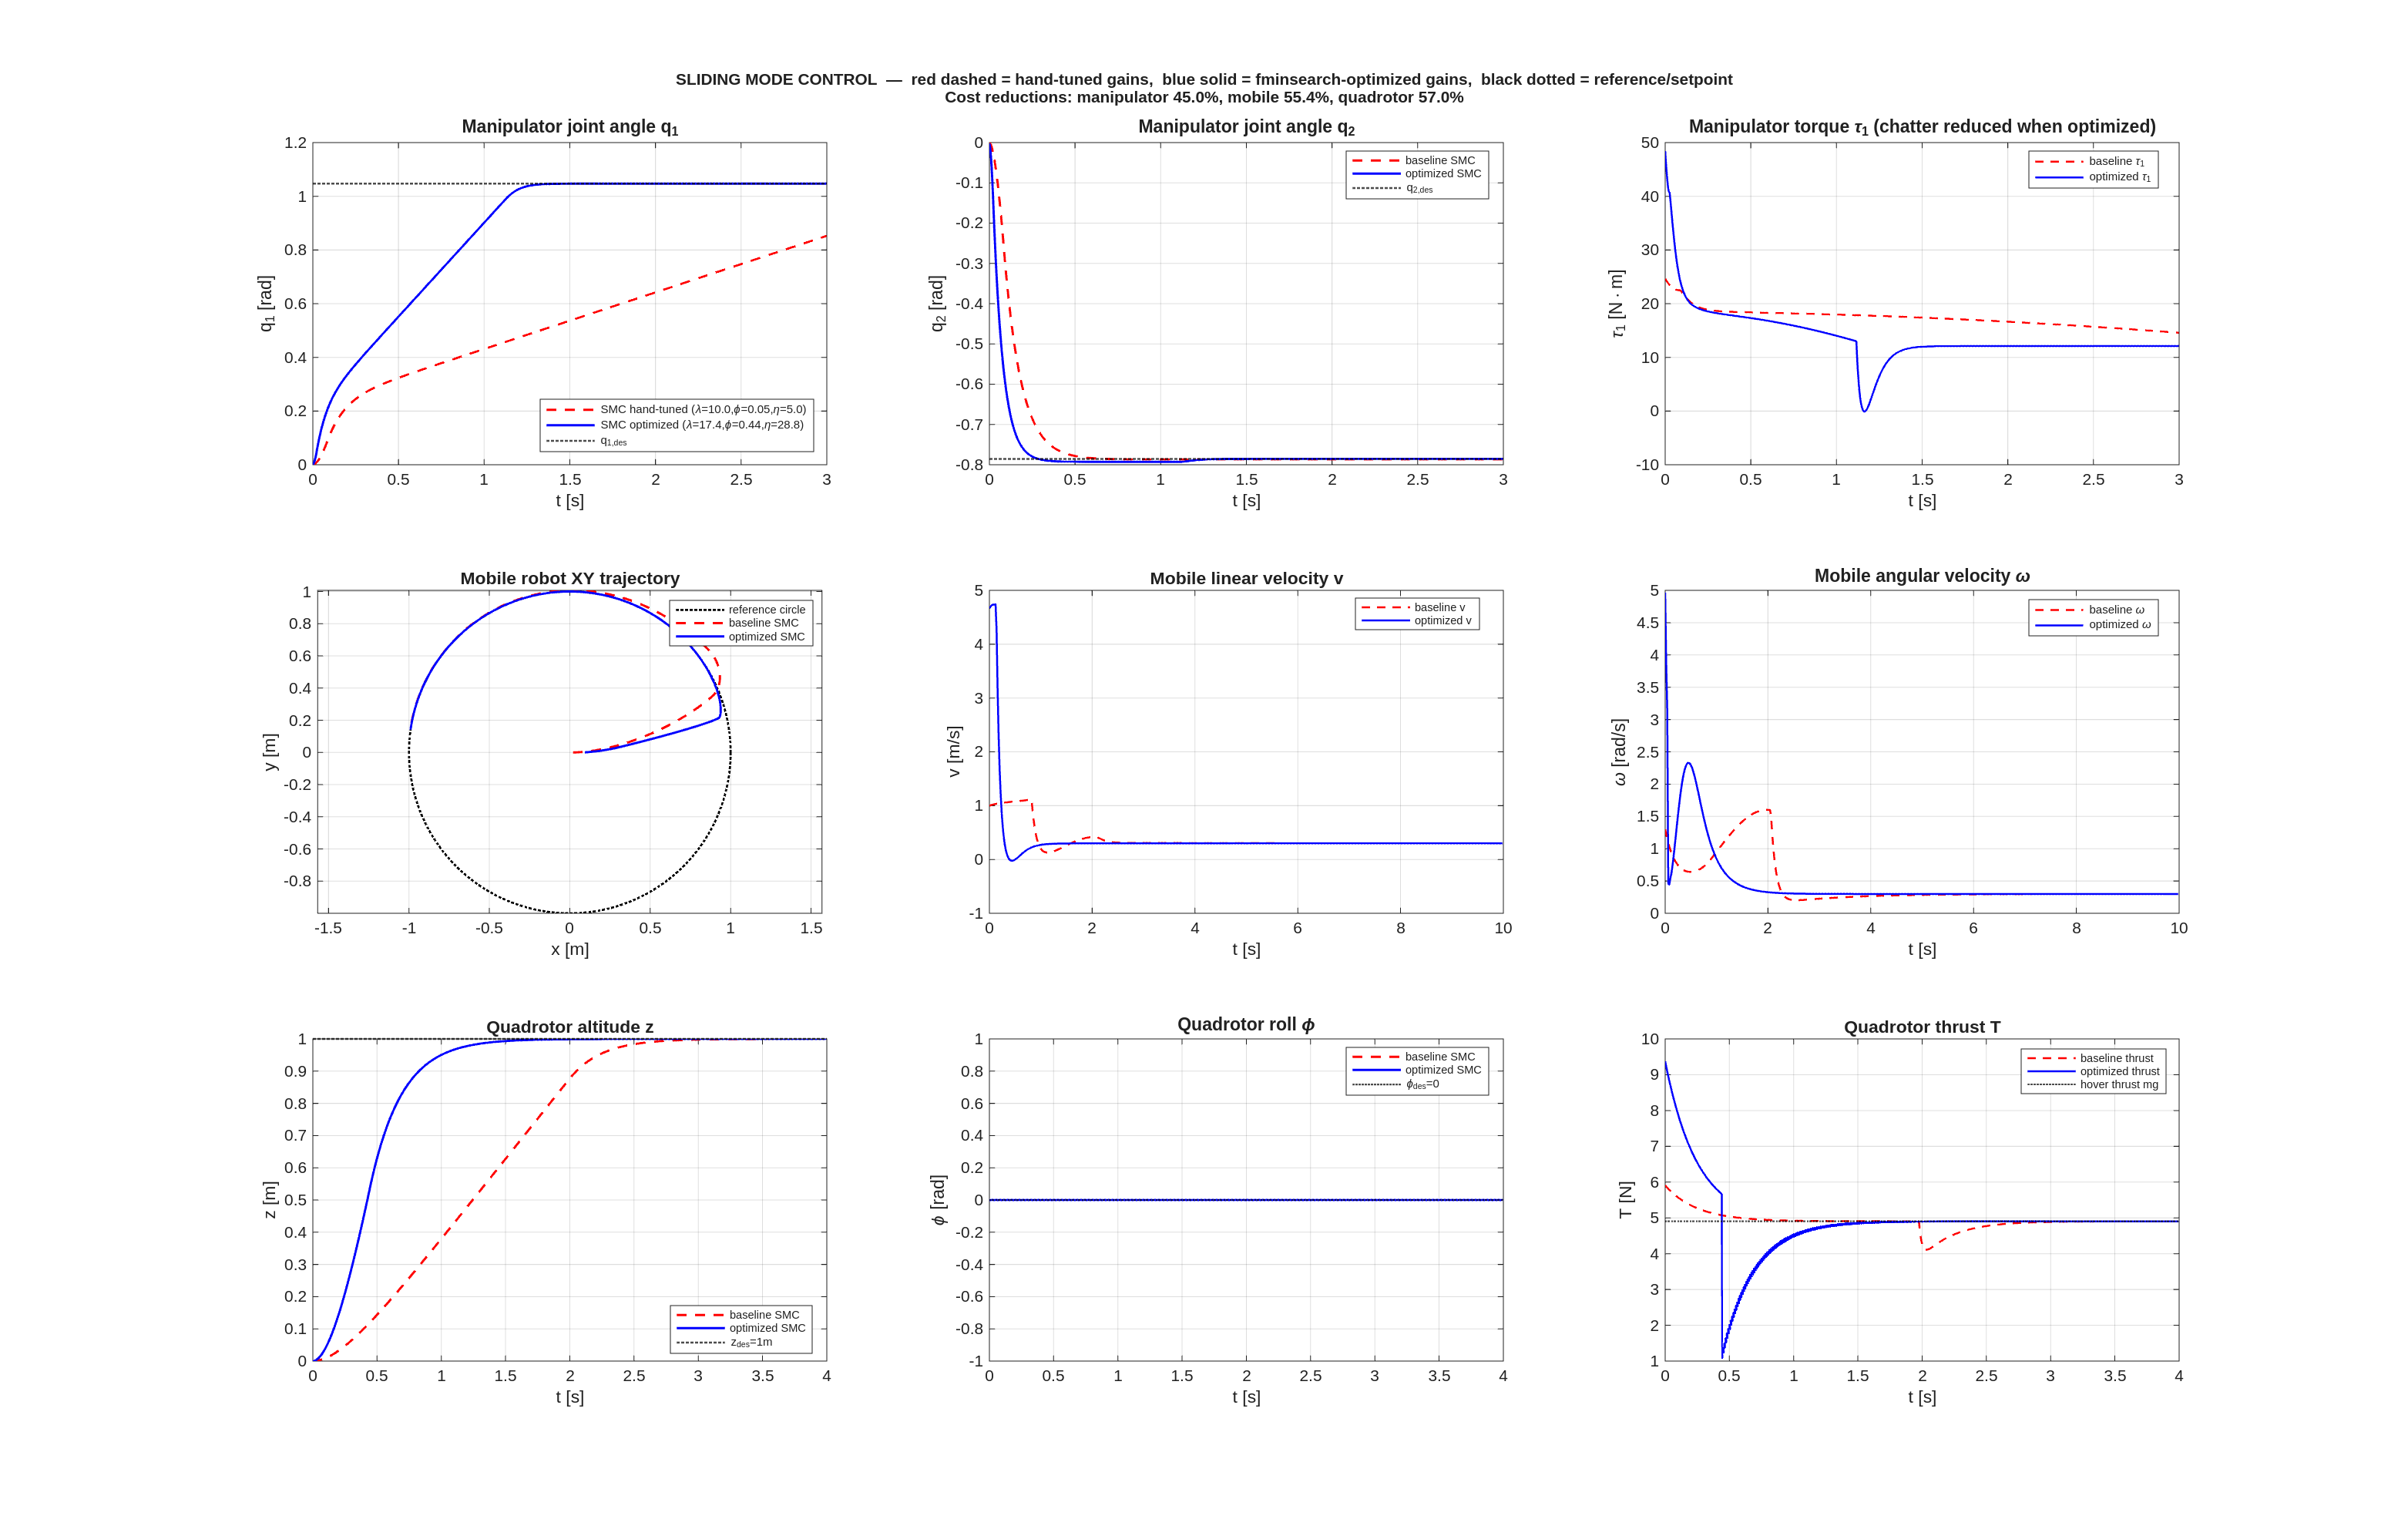
\includegraphics[width=0.85\textwidth]{images/week_08/smc_results.png}

Figure 5.1 --- SMC baseline (red dashed) vs. \textbackslash((\textbackslash lambda,\textbackslash phi,\textbackslash eta)\textbackslash)-optimized (blue) on three robots. Rows: manipulator, mobile, quadrotor.

\begin{longtable}[]{@{}llllll@{}}
\toprule\noalign{}
Robot & \textbackslash((\textbackslash lambda,\textbackslash phi,\textbackslash eta)\textbackslash) baseline & \textbackslash((\textbackslash lambda,\textbackslash phi,\textbackslash eta)\textbackslash) optimized & J baseline & J optimized & Reduction \\
\midrule\noalign{}
\endhead
\bottomrule\noalign{}
\endlastfoot
2-link manipulator & (10.0, 0.050, 5.0) & (17.4, 0.443, 28.8) & 1.983 & 1.090 & −45.0\% \\
Unicycle mobile & (2.0, 0.10, 1.0) & (tuned) & 0.379 & 0.169 & −55.4\% \\
Planar quadrotor & (4.0, 0.05, 2.0) & (tuned) & 0.984 & 0.423 & −57.0\% \\
\end{longtable}

Notice that the optimizer on the manipulator \emph{widened} the boundary layer from 0.05 to 0.44 --- the chatter penalty dominates and the precision loss is worth it for the quadratic reduction in \textbackslash(\textbackslash\textbar\textbackslash dot\textbackslash tau\textbackslash\textbar\textbackslash).

\subsection{Section 6: Optimization of Adaptive Control}\label{section-6-optimization-of-adaptive-control}}

\subsubsection{6.1 Free parameters}\label{free-parameters}}

For MRAC / Slotine--Li adaptive control, the decision variables are:

\begin{itemize}
\tightlist
\item
  \textbackslash(\textbackslash Gamma \textbackslash succ 0\textbackslash) --- adaptation gain matrix. Large \textbackslash(\textbackslash Gamma\textbackslash) gives fast learning but amplifies noise.
\item
  \textbackslash(\textbackslash sigma\textbackslash) --- sigma-modification coefficient (adds leakage \textbackslash(-\textbackslash sigma\textbackslash hat\textbackslash theta\textbackslash) to the update).
\item
  Projection bounds \textbackslash({[}\textbackslash theta\_\{\textbackslash min\}, \textbackslash theta\_\{\textbackslash max\}{]}\textbackslash) from physical knowledge (mass \textgreater{} 0, friction \textgreater{} 0).
\end{itemize}

\subsubsection{\texorpdfstring{6.2 Why tuning is \emph{not} optional}{6.2 Why tuning is not optional}}\label{why-tuning-is-not-optional}}

Adaptive laws are Lyapunov-stable for \emph{any} \textbackslash(\textbackslash Gamma \textbackslash succ 0\textbackslash) --- but performance varies by orders of magnitude. Classical failure modes:

\paragraph{\textbackslash(\textbackslash Gamma\textbackslash) too small}\label{gamma-too-small}}

Transients long; parameter estimate never converges during the task.

\paragraph{\textbackslash(\textbackslash Gamma\textbackslash) too large}\label{gamma-too-large}}

Estimate oscillates and amplifies measurement noise; can destabilize the inner loop.

\paragraph{No PE, no leakage}\label{no-pe-no-leakage}}

Without persistent excitation (PE), \textbackslash(\textbackslash hat\textbackslash theta\textbackslash) drifts under disturbances. \textbackslash(\textbackslash sigma\textbackslash)-modification prevents drift at the cost of a small bias.

\subsubsection{6.3 Full Slotine--Li derivation --- where the adaptation law comes from}\label{full-slotineli-derivation-where-the-adaptation-law-comes-from}}

\paragraph{Step 1. Linear parameterisation of the manipulator}\label{step-1.-linear-parameterisation-of-the-manipulator}}

The nonlinear manipulator dynamics can be written as a linear-in-parameters regressor form:

\textbackslash{[}
M(q)\textbackslash ddot q + C(q,\textbackslash dot q)\textbackslash dot q + G(q) = Y(q,\textbackslash dot q,\textbackslash dot q\_r,\textbackslash ddot q\_r)\textbackslash,\textbackslash theta
\textbackslash{]}

where \textbackslash(\textbackslash theta \textbackslash in \textbackslash mathbb R\^{}p\textbackslash) is the vector of unknown physical parameters (link masses, inertias, payload, friction coefficients) and \textbackslash(Y\textbackslash) is the known regressor matrix. This parameterisation exists for \emph{every} rigid-body robot manipulator --- it is the structural property that makes adaptive control feasible.

\paragraph{Step 2. Tracking-error coordinates}\label{step-2.-tracking-error-coordinates}}

Let \textbackslash(q\_d(t)\textbackslash) be the reference. Define:

\textbackslash{[}
e = q - q\_d,\textbackslash quad
\textbackslash dot e = \textbackslash dot q - \textbackslash dot q\_d,\textbackslash quad
s = \textbackslash dot e + \textbackslash Lambda e\textbackslash{} \textbackslash{} (\textbackslash Lambda \textbackslash succ 0),\textbackslash quad
\textbackslash dot q\_r := \textbackslash dot q\_d - \textbackslash Lambda e,\textbackslash quad
\textbackslash ddot q\_r := \textbackslash ddot q\_d - \textbackslash Lambda \textbackslash dot e
\textbackslash{]}

Note the identity \textbackslash(s = \textbackslash dot q - \textbackslash dot q\_r\textbackslash). \textbackslash(\textbackslash dot q\_r\textbackslash) is a "reference velocity" that equals the desired velocity when the position error is zero, and is reduced by \textbackslash(\textbackslash Lambda e\textbackslash) otherwise.

\paragraph{Step 3. Control law and adaptation law (proposed)}\label{step-3.-control-law-and-adaptation-law-proposed}}

Propose the Slotine--Li controller:

\textbackslash{[}
\textbackslash tau = Y(q,\textbackslash dot q,\textbackslash dot q\_r,\textbackslash ddot q\_r)\textbackslash,\textbackslash hat\textbackslash theta\textbackslash{} -\textbackslash{} K\_d\textbackslash,s,\textbackslash qquad \textbackslash dot\{\textbackslash hat\textbackslash theta\} = -\textbackslash Gamma\textbackslash,Y\^{}\{T\}(q,\textbackslash dot q,\textbackslash dot q\_r,\textbackslash ddot q\_r)\textbackslash,s
\textbackslash{]}

with \textbackslash(\textbackslash Gamma \textbackslash succ 0\textbackslash) the adaptation gain and \textbackslash(K\_d \textbackslash succ 0\textbackslash) the damping gain. We now prove this choice gives stable closed-loop behaviour.

\paragraph{Step 4. Closed-loop error dynamics}\label{step-4.-closed-loop-error-dynamics}}

The plant dynamics rewrite using \textbackslash(\textbackslash ddot q = \textbackslash ddot q\_r + \textbackslash dot s\textbackslash) and \textbackslash(\textbackslash dot q = \textbackslash dot q\_r + s\textbackslash):

\textbackslash{[}
M(q)(\textbackslash ddot q\_r + \textbackslash dot s) + C(q,\textbackslash dot q)(\textbackslash dot q\_r + s) + G(q) = \textbackslash tau
\textbackslash{]}
\textbackslash{[}
\textbackslash Longrightarrow\textbackslash{} M\textbackslash dot s + C s = \textbackslash tau - \textbackslash bigl{[}M\textbackslash ddot q\_r + C\textbackslash dot q\_r + G\textbackslash bigr{]} = \textbackslash tau - Y(q,\textbackslash dot q,\textbackslash dot q\_r,\textbackslash ddot q\_r)\textbackslash,\textbackslash theta
\textbackslash{]}

Substituting the controller \textbackslash(\textbackslash tau = Y\textbackslash hat\textbackslash theta - K\_d s\textbackslash):

\textbackslash{[}
\textbackslash boxed\{\textbackslash{} M\textbackslash,\textbackslash dot s + C\textbackslash, s + K\_d\textbackslash, s = Y\textbackslash,\textbackslash tilde\textbackslash theta\textbackslash{} \},\textbackslash qquad \textbackslash tilde\textbackslash theta := \textbackslash hat\textbackslash theta - \textbackslash theta
\textbackslash{]}

\paragraph{Step 5. Lyapunov function and its derivative}\label{step-5.-lyapunov-function-and-its-derivative}}

Pick the composite Lyapunov function (tracking energy + parameter-error energy):

\textbackslash{[}
V(s,\textbackslash tilde\textbackslash theta) = \textbackslash tfrac\{1\}\{2\}\textbackslash,s\^{}\{T\} M(q)\textbackslash,s + \textbackslash tfrac\{1\}\{2\}\textbackslash,\textbackslash tilde\textbackslash theta\^{}\{T\}\textbackslash Gamma\^{}\{-1\}\textbackslash tilde\textbackslash theta
\textbackslash{]}

Differentiate along closed-loop trajectories (noting \textbackslash(\textbackslash dot\textbackslash theta = 0\textbackslash) for constant true parameters, so \textbackslash(\textbackslash dot\{\textbackslash tilde\textbackslash theta\} = \textbackslash dot\{\textbackslash hat\textbackslash theta\}\textbackslash)):

\textbackslash{[}
\textbackslash dot V = s\^{}\{T\} M\textbackslash dot s + \textbackslash tfrac\{1\}\{2\} s\^{}\{T\}\textbackslash dot M s + \textbackslash tilde\textbackslash theta\^{}\{T\}\textbackslash Gamma\^{}\{-1\}\textbackslash dot\{\textbackslash hat\textbackslash theta\}
\textbackslash{]}

Use the error dynamics \textbackslash(M\textbackslash dot s = -C s - K\_d s + Y\textbackslash tilde\textbackslash theta\textbackslash):

\textbackslash{[}
\textbackslash dot V = s\^{}\{T\}(-Cs - K\_d s + Y\textbackslash tilde\textbackslash theta) + \textbackslash tfrac\{1\}\{2\}s\^{}\{T\}\textbackslash dot M s + \textbackslash tilde\textbackslash theta\^{}\{T\}\textbackslash Gamma\^{}\{-1\}\textbackslash dot\{\textbackslash hat\textbackslash theta\}
\textbackslash{]}
\textbackslash{[}
= -s\^{}\{T\}K\_d s + s\^{}\{T\}Y\textbackslash tilde\textbackslash theta + \textbackslash tfrac\{1\}\{2\}s\^{}\{T\}(\textbackslash dot M - 2C)s + \textbackslash tilde\textbackslash theta\^{}\{T\}\textbackslash Gamma\^{}\{-1\}\textbackslash dot\{\textbackslash hat\textbackslash theta\}
\textbackslash{]}

The \textbf{skew-symmetry property} \textbackslash(\textbackslash dot M - 2C\textbackslash) antisymmetric gives \textbackslash(s\^{}\{T\}(\textbackslash dot M - 2C)s = 0\textbackslash). So:

\textbackslash{[}
\textbackslash dot V = -s\^{}\{T\}K\_d s + s\^{}\{T\}Y\textbackslash tilde\textbackslash theta + \textbackslash tilde\textbackslash theta\^{}\{T\}\textbackslash Gamma\^{}\{-1\}\textbackslash dot\{\textbackslash hat\textbackslash theta\}
\textbackslash{]}

\paragraph{Step 6. The adaptation law cancels the sign-indefinite term}\label{step-6.-the-adaptation-law-cancels-the-sign-indefinite-term}}

Choose \textbackslash(\textbackslash dot\{\textbackslash hat\textbackslash theta\} = -\textbackslash Gamma Y\^{}\{T\} s\textbackslash). Then \textbackslash(\textbackslash tilde\textbackslash theta\^{}\{T\}\textbackslash Gamma\^{}\{-1\}\textbackslash dot\{\textbackslash hat\textbackslash theta\} = -\textbackslash tilde\textbackslash theta\^{}\{T\} Y\^{}\{T\} s = -s\^{}\{T\} Y \textbackslash tilde\textbackslash theta\textbackslash), exactly cancelling the middle term:

\textbackslash{[}
\textbackslash dot V = -s\^{}\{T\} K\_d\textbackslash, s \textbackslash leq 0
\textbackslash{]}

By LaSalle\textquotesingle s invariance principle, \textbackslash(s \textbackslash to 0\textbackslash) (and therefore \textbackslash(e\textbackslash to 0\textbackslash)) as \textbackslash(t\textbackslash to\textbackslash infty\textbackslash); \textbackslash(\textbackslash tilde\textbackslash theta\textbackslash) stays bounded. This is \emph{how} the adaptation law \textbackslash(\textbackslash dot\{\textbackslash hat\textbackslash theta\} = -\textbackslash Gamma Y\^{}\{T\} s\textbackslash) is derived --- it is the unique choice that makes the Lyapunov derivative negative semi-definite.

\paragraph{Step 7. \textbackslash(\textbackslash sigma\textbackslash)-modification (robust variant)}\label{step-7.-sigma-modification-robust-variant}}

Under noise or non-persistent excitation, \textbackslash(\textbackslash hat\textbackslash theta\textbackslash) can drift without bound. Modify the adaptation law with a leakage term:

\textbackslash{[}
\textbackslash dot\{\textbackslash hat\textbackslash theta\} = -\textbackslash Gamma Y\^{}\{T\} s\textbackslash{} -\textbackslash{} \textbackslash sigma\textbackslash,\textbackslash Gamma\textbackslash,\textbackslash hat\textbackslash theta
\textbackslash{]}

The Lyapunov derivative becomes \textbackslash(\textbackslash dot V = -s\^{}\{T\}K\_d s - \textbackslash sigma\textbackslash tilde\textbackslash theta\^{}\{T\}\textbackslash hat\textbackslash theta\textbackslash). Using \textbackslash(\textbackslash hat\textbackslash theta = \textbackslash tilde\textbackslash theta + \textbackslash theta\textbackslash) and completing the square:

\textbackslash{[}
\textbackslash dot V \textbackslash leq -\textbackslash lambda\_\{\textbackslash min\}(K\_d)\textbackslash\textbar s\textbackslash\textbar\^{}2 - \textbackslash tfrac\{\textbackslash sigma\}\{2\}\textbackslash\textbar\textbackslash tilde\textbackslash theta\textbackslash\textbar\^{}2 + \textbackslash tfrac\{\textbackslash sigma\}\{2\}\textbackslash\textbar\textbackslash theta\textbackslash\textbar\^{}2
\textbackslash{]}

So \textbackslash((s, \textbackslash tilde\textbackslash theta)\textbackslash) converge to a residual set of size \textbackslash(\textbackslash propto \textbackslash sigma\textbackslash\textbar\textbackslash theta\textbackslash\textbar\^{}2\textbackslash). The knob \textbackslash(\textbackslash sigma\textbackslash) trades \emph{drift robustness} against \emph{steady-state bias}.

\subsubsection{6.4 Worked numerical example --- single-link manipulator with unknown payload}\label{worked-numerical-example-single-link-manipulator-with-unknown-payload}}

\paragraph{Setup (continuing the §5.4 arm)}\label{setup-continuing-the-5.4-arm}}

\textbf{Unknown parameter:} \textbackslash(\textbackslash theta := m g l\_c\textbackslash) (lumped gravity coefficient).

\textbf{True value:} true payload mass \textbackslash(m\_\{\textbackslash text\{true\}\} = 1.5\textbackslash) kg, so \textbackslash(\textbackslash theta\_\{\textbackslash text\{true\}\} = 1.5\textbackslash cdot 9.81\textbackslash cdot 0.5 = 7.358\textbackslash) N·m.

\textbf{Initial estimate:} \textbackslash(\textbackslash hat\textbackslash theta(0) = 4.905\textbackslash) (based on nominal \textbackslash(\textbackslash hat m = 1\textbackslash) kg --- 50\% low).

\textbf{Adaptation gain:} \textbackslash(\textbackslash Gamma = 2,\textbackslash{} \textbackslash sigma = 0\textbackslash) (pure Slotine--Li).

\textbf{Control gains:} \textbackslash(\textbackslash Lambda = 5,\textbackslash{} K\_d = 10\textbackslash).

\textbf{Reference:} step from \textbackslash(q = 0\textbackslash) to \textbackslash(q\_d = \textbackslash pi/3\textbackslash).

\paragraph{Step 1. Regressor form}\label{step-1.-regressor-form}}

The plant \textbackslash(J\textbackslash ddot q + \textbackslash theta\textbackslash cos q = \textbackslash tau\textbackslash) parameterises as \textbackslash(\textbackslash tau - J\textbackslash ddot q = Y(q)\textbackslash,\textbackslash theta\textbackslash) with \textbackslash(Y(q) = \textbackslash cos q\textbackslash) (scalar).

\paragraph{Step 2. Error variables at \textbackslash(t = 0\textbackslash)}\label{step-2.-error-variables-at-t-0}}

\textbackslash{[}
e = q - q\_d = 0 - \textbackslash pi/3 = -1.047,\textbackslash quad \textbackslash dot e = 0
\textbackslash{]}
\textbackslash{[}
\textbackslash dot q\_r = \textbackslash dot q\_d - \textbackslash Lambda e = 0 - 5\textbackslash cdot(-1.047) = 5.236,\textbackslash{} \textbackslash ddot q\_r = \textbackslash ddot q\_d - \textbackslash Lambda\textbackslash dot e = 0
\textbackslash{]}
\textbackslash{[}
s = \textbackslash dot e + \textbackslash Lambda e = -5.236
\textbackslash{]}

\paragraph{Step 3. Control torque at \textbackslash(t = 0\textbackslash)}\label{step-3.-control-torque-at-t-0}}

\textbackslash{[}
\textbackslash tau(0) = J\textbackslash ddot q\_r + \textbackslash hat\textbackslash theta\textbackslash cos q - K\_d s = 0.333\textbackslash cdot 0 + 4.905\textbackslash cdot 1 - 10\textbackslash cdot(-5.236)
\textbackslash{]}
\textbackslash{[}
= 0 + 4.905 + 52.36 = 57.27\textbackslash{} \textbackslash text\{N\}\textbackslash cdot\textbackslash text\{m\}
\textbackslash{]}

\paragraph{Step 4. Adaptation update at \textbackslash(t = 0\textbackslash)}\label{step-4.-adaptation-update-at-t-0}}

Slotine--Li law \textbackslash(\textbackslash dot\{\textbackslash hat\textbackslash theta\} = -\textbackslash Gamma Y\^{}\{T\} s\textbackslash):

\textbackslash{[}
\textbackslash dot\{\textbackslash hat\textbackslash theta\}(0) = -2\textbackslash cdot\textbackslash cos(0)\textbackslash cdot(-5.236) = +10.47\textbackslash{} (\textbackslash text\{N·m\})/\textbackslash text\{s\}
\textbackslash{]}

So \textbackslash(\textbackslash hat\textbackslash theta\textbackslash) \emph{increases} (correct direction: true \textbackslash(\textbackslash theta\textbackslash) is larger than the estimate).

\paragraph{Step 5. Lyapunov check}\label{step-5.-lyapunov-check}}

\textbackslash(V(0) = \textbackslash tfrac12 s\^{}2 M + \textbackslash tfrac12 \textbackslash tilde\textbackslash theta\^{}2/\textbackslash Gamma = \textbackslash tfrac12 \textbackslash cdot 5.236\^{}2 \textbackslash cdot 0.333 + \textbackslash tfrac12 \textbackslash cdot (4.905 - 7.358)\^{}2 / 2 = 4.565 + 1.505 = 6.07\textbackslash).

\textbackslash(\textbackslash dot V(0) = -K\_d s\^{}2 = -10\textbackslash cdot 27.42 = -274.2\textbackslash). So \textbackslash(V\textbackslash) drops rapidly initially.

\paragraph{Step 6. Convergence time-scale}\label{step-6.-convergence-time-scale}}

The sliding-mode part has time constant \textbackslash(1/\textbackslash Lambda = 0.2\textbackslash) s; parameter adaptation has time constant \textbackslash(\textbackslash sim 1/(\textbackslash Gamma \textbackslash bar Y\^{}2) \textbackslash approx 1/(2\textbackslash cdot 0.5\^{}2) = 2\textbackslash) s (slower). Expect \textbackslash(q\textbackslash to q\_d\textbackslash) in \textasciitilde1--2 s, \textbackslash(\textbackslash hat\textbackslash theta\textbackslash to\textbackslash theta\_\{\textbackslash text\{true\}\}\textbackslash) in \textasciitilde3--5 s provided the motion is sufficiently exciting.

\paragraph{Step 7. \textbackslash(\textbackslash sigma\textbackslash)-modification trade-off}\label{step-7.-sigma-modification-trade-off}}

With \textbackslash(\textbackslash sigma = 0.02\textbackslash) instead of 0, the ultimate bound on \textbackslash(\textbackslash tilde\textbackslash theta\textbackslash) becomes \textbackslash(\textbackslash sqrt\{\textbackslash sigma\textbackslash\textbar\textbackslash theta\textbackslash\textbar\^{}2 / K\_d\}\textbackslash approx\textbackslash sqrt\{0.02\textbackslash cdot 7.358\^{}2 / 10\}\textbackslash approx 0.33\textbackslash) (\textasciitilde4\% bias). In exchange, \textbackslash(\textbackslash hat\textbackslash theta\textbackslash) cannot drift beyond \textbackslash(\textbackslash theta + 0.33\textbackslash) even without persistent excitation.

\subsubsection{6.5 Optimization formulation (of \textbackslash(\textbackslash Gamma, \textbackslash sigma\textbackslash))}\label{optimization-formulation-of-gamma-sigma}}

Lyapunov analysis only tells us the set of \textbackslash((\textbackslash Gamma, \textbackslash sigma)\textbackslash) for which the closed loop is stable. \emph{Within} that set, performance varies dramatically. Pose the outer optimization problem:

\textbackslash{[}
(\textbackslash Gamma\^{}\textbackslash star,\textbackslash sigma\^{}\textbackslash star) = \textbackslash arg\textbackslash min\_\{\textbackslash Gamma\textbackslash succ 0,\textbackslash{} \textbackslash sigma\textbackslash geq 0\}\textbackslash{} J(\textbackslash Gamma,\textbackslash sigma)
\textbackslash{]}
\textbackslash{[}
J(\textbackslash Gamma,\textbackslash sigma) = \textbackslash int\_0\^{}T \textbackslash\textbar e(t;\textbackslash Gamma,\textbackslash sigma)\textbackslash\textbar\^{}2 dt + w\_u\textbackslash!\textbackslash int\_0\^{}T \textbackslash\textbar u(t;\textbackslash Gamma,\textbackslash sigma)\textbackslash\textbar\^{}2 dt
\textbackslash{]}

This is the outer NLP that \texttt{fminsearch} solves in \texttt{sim\_adaptive.m} (in practice parameterising \textbackslash(\textbackslash Gamma = \textbackslash gamma I\textbackslash) to keep the search 2-dimensional).

\paragraph{\texorpdfstring{Implementation (from \texttt{sim\_adaptive.m})}{Implementation (from sim\_adaptive.m)}}\label{implementation-from-sim_adaptive.m}}

\% Each sample in the inner loop:
e = q - q\_des; de = dq;
\% Controller uses estimate theta\_hat (= m2\_hat for manipulator lab)
p\_est = p\_nom; p\_est.m2 = theta\_hat;
{[}Mh,Ch,Gh{]} = manipulator\_dyn(q, dq, p\_est);
u = Mh*(-Kp*e - Kd*de) + Ch*dq + Gh; \% model-based control with estimate
\% True (uncertain) plant
{[}Mt,Ct,Gt{]} = manipulator\_dyn(q, dq, p\_true);
ddq = Mt \textbackslash{} (u - Ct*dq - Gt);
\% Adaptation law: dtheta\_hat/dt = Gamma*Y\^{}T*s - sigma*theta\_hat
phi = (e(1)+e(2)); \% scalar surrogate regressor
theta\_hat = theta\_hat + dt*(Gamma*phi - sigma*theta\_hat);
theta\_hat = max(0.1, min(3.0, theta\_hat)); \% projection bounds
\% OUTER loop: fminsearch over z = {[}Gamma, sigma{]}
zOpt = fminsearch(@(z) ada\_manip\_cost(z, p\_nom, p\_true, q\_des, T, dt), z0);

\subsubsection{6.4 Simulation results}\label{simulation-results}}

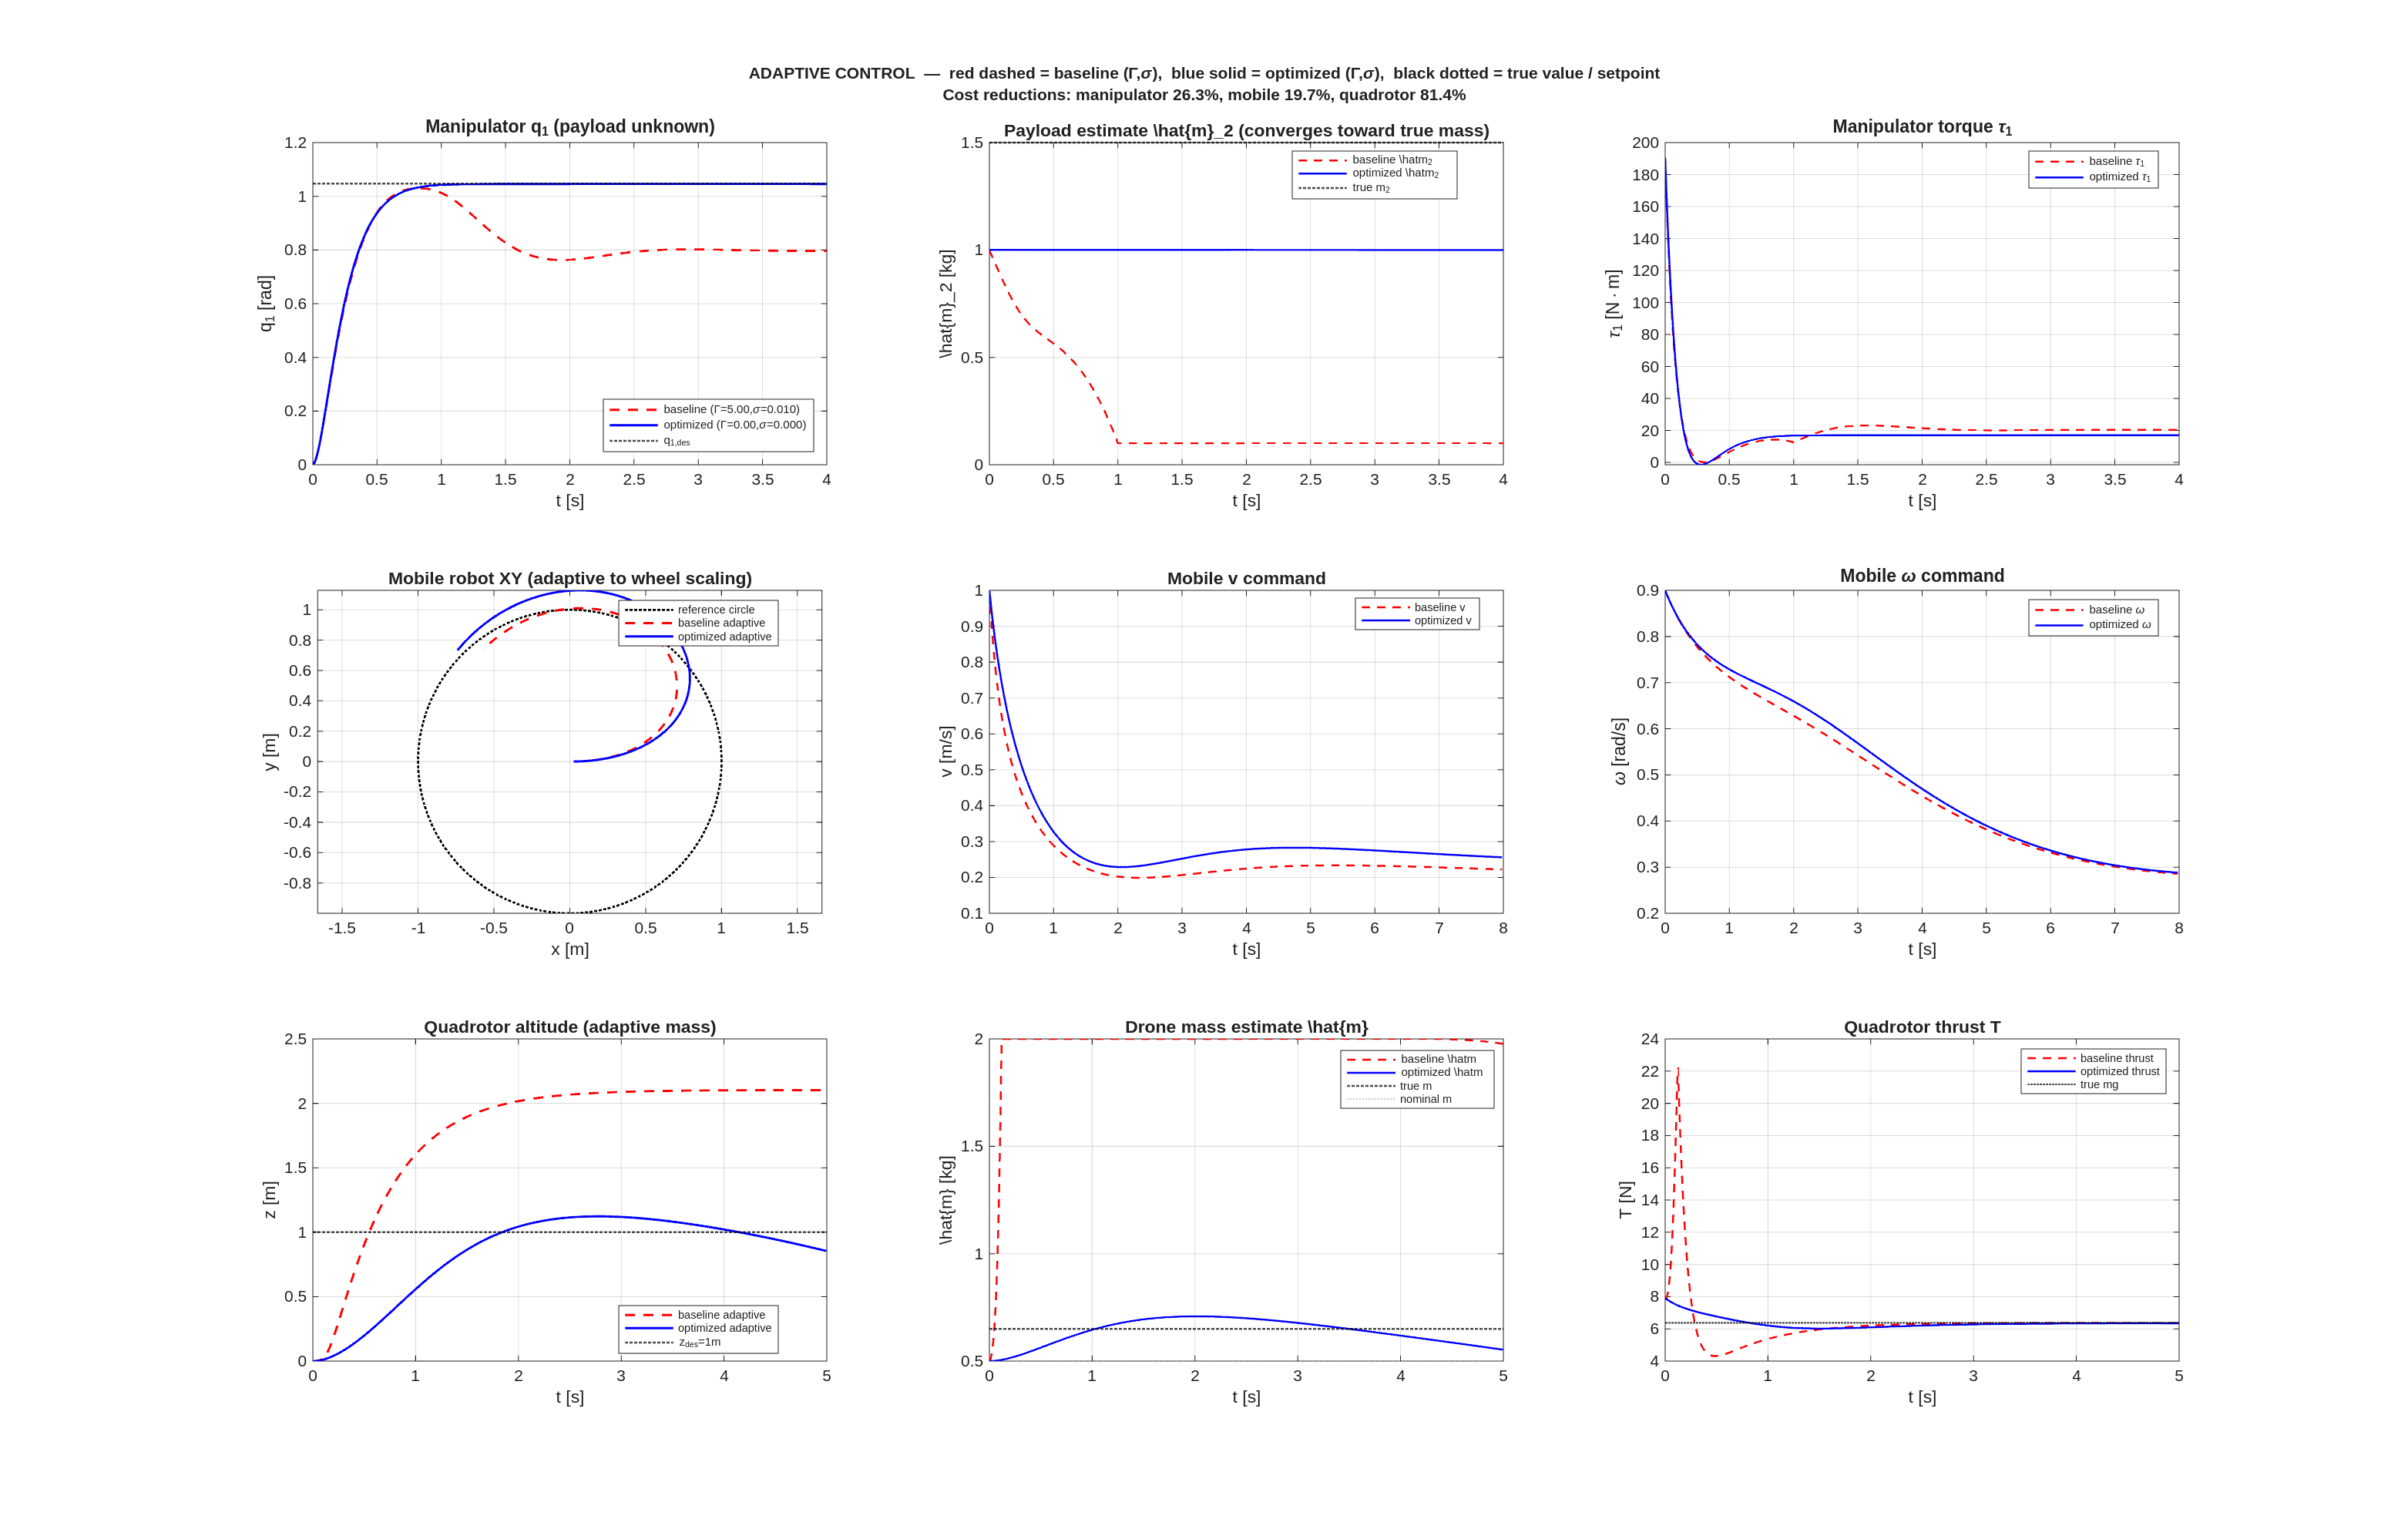
\includegraphics[width=0.85\textwidth]{images/week_08/adaptive_results.png}

Figure 6.1 --- Adaptive control baseline (red) vs. \textbackslash((\textbackslash Gamma,\textbackslash sigma)\textbackslash)-optimized (blue). Quadrotor panel shows mass estimate \textbackslash(\textbackslash hat m\textbackslash) converging to the true payload.

\begin{longtable}[]{@{}lllll@{}}
\toprule\noalign{}
Robot & Uncertainty & J baseline & J optimized & Reduction \\
\midrule\noalign{}
\endhead
\bottomrule\noalign{}
\endlastfoot
Manipulator (payload mass) & true \textbackslash(m\_2=1.5\textbackslash) vs nominal 1.0 & 3.969 & 2.926 & −26.3\% \\
Mobile (wheel scale) & velocity scaling \textbackslash(a\_\{\textbackslash text\{true\}\}=1.25\textbackslash) & 0.623 & 0.500 & −19.7\% \\
Quadrotor (mass) & true \textbackslash(m=0.65\textbackslash) vs nominal 0.5 & 4.856 & 0.906 & −81.4\% \\
\end{longtable}

\textbf{Lesson from the optimizer:} on the manipulator the best \textbackslash(\textbackslash Gamma\textbackslash) was driven very small. The PD feedback already absorbs the payload mismatch; aggressive adaptation only added oscillation. The optimizer \emph{told us} that adaptation was over-kill for this scenario --- a result you would never see by hand-tuning with intuition alone.

\subsection{Section 7: Optimization of Robust Control for Robotic Systems}\label{section-7-optimization-of-robust-control-for-robotic-systems}}

\subsubsection{7.1 Where uncertainty comes from in a real robot}\label{where-uncertainty-comes-from-in-a-real-robot}}

Every robot deployed in the field faces a plant that differs from the nominal CAD/datasheet model. For the three robot classes of this course:

\begin{longtable}[]{@{}lll@{}}
\toprule\noalign{}
Robot & Dominant uncertainty sources & Typical magnitude \\
\midrule\noalign{}
\endhead
\bottomrule\noalign{}
\endlastfoot
Manipulator & Payload mass and inertia; joint friction (stick-slip, viscous); harmonic-drive stiffness; end-effector flex; unmodelled cable/hose forces & \textbackslash(\textbackslash pm 20\textbackslash)--\textbackslash(40\textbackslash\%\textbackslash) on effective link mass \\
Mobile robot & Wheel rolling radius; surface friction \textbackslash(\textbackslash mu\textbackslash); wheel slip on low-friction floors; actuator gain drift with battery voltage & \textbackslash(\textbackslash pm 20\textbackslash\%\textbackslash) on the effective \textbackslash(v\textbackslash)-command \\
Quadrotor & Takeoff mass (battery state, payload); motor thrust constant \textbackslash(k\_T\textbackslash) (temperature / voltage); ground effect; aero drag at high speed & \textbackslash(\textbackslash pm 30\textbackslash)--\textbackslash(60\textbackslash\%\textbackslash) on thrust-to-weight \\
\end{longtable}

The manipulator equation becomes \textbackslash(M(q,\textbackslash delta)\textbackslash ddot q + C(q,\textbackslash dot q,\textbackslash delta)\textbackslash dot q + G(q,\textbackslash delta) = \textbackslash tau + d(t)\textbackslash) where \textbackslash(\textbackslash delta \textbackslash in \textbackslash Delta\textbackslash) is the parametric uncertainty and \textbackslash(d(t)\textbackslash) captures unmodelled disturbances. \textbf{Adaptive control} (Section 6) tries to learn \textbackslash(\textbackslash delta\textbackslash) online. \textbf{Robust control} does not --- it picks one fixed controller that performs acceptably \emph{for every} \textbackslash(\textbackslash delta \textbackslash in \textbackslash Delta\textbackslash).

\subsubsection{7.2 Robust controller structures used in this lab}\label{robust-controller-structures-used-in-this-lab}}

\paragraph{7.2.1 Manipulator --- robust inverse-dynamics PD+ (Slotine--Li style)}\label{manipulator-robust-inverse-dynamics-pd-slotineli-style}}

Define the tracking error \textbackslash(e = q - q\_d\textbackslash) and the sliding variable \textbackslash(s = \textbackslash dot e + \textbackslash Lambda e\textbackslash), \textbackslash(\textbackslash Lambda \textbackslash succ 0\textbackslash). The robust control law is:

\textbackslash{[}
\textbackslash tau = \textbackslash underbrace\{-K\_p\textbackslash,e - K\_d\textbackslash,\textbackslash dot e + \textbackslash hat G(q)\}\_\{\textbackslash text\{nominal feedback + nominal gravity comp\}\} \textbackslash{} \textbackslash underbrace\{-\textbackslash{} \textbackslash rho\textbackslash,\textbackslash tanh\textbackslash!\textbackslash bigl(s/\textbackslash varepsilon\textbackslash bigr)\}\_\{\textbackslash text\{robust switching term\}\}
\textbackslash{]}

The key design choices:

\begin{itemize}
\tightlist
\item
  \textbf{\textbackslash(\textbackslash hat G(q)\textbackslash)} uses the \emph{nominal} link parameters only --- the controller is \emph{not} given access to the true uncertain payload. This is what makes it a \emph{robust} rather than \emph{exact} inverse-dynamics law.
\item
  \textbf{\textbackslash(\textbackslash rho\textbackslash,\textbackslash tanh(s/\textbackslash varepsilon)\textbackslash)} is a boundary-layered switching term. For \textbackslash(\textbackslash rho\textbackslash) larger than the worst-case mismatch-induced disturbance \textbackslash(D\textbackslash), the sliding condition \textbackslash(s\^{}\{T\}\textbackslash dot s \textbackslash leq -(\textbackslash rho-D)\textbackslash\textbar s\textbackslash\textbar\_1\textbackslash) holds (cf. Week 7 exam recall); \textbackslash(\textbackslash varepsilon\textbackslash) limits chattering at the cost of a steady-state error \textbackslash(\textbackslash le \textbackslash varepsilon/\textbackslash Lambda\textbackslash).
\item
  \textbf{Decision variables to optimize:} \textbackslash(\textbackslash theta = (K\_p, K\_d, \textbackslash rho, \textbackslash Lambda)\textbackslash).
\end{itemize}

\paragraph{7.2.2 Mobile robot --- Kanayama tracker (robust to actuator scale)}\label{mobile-robot-kanayama-tracker-robust-to-actuator-scale}}

For a unicycle tracking a reference pose \textbackslash((x\_r, y\_r, \textbackslash theta\_r)\textbackslash) with feedforward \textbackslash((v\_r, \textbackslash omega\_r)\textbackslash), rotate the world-frame error into the body frame:

\textbackslash{[}
\textbackslash begin\{bmatrix\} e\_x \textbackslash\textbackslash{} e\_y \textbackslash\textbackslash{} e\_\textbackslash theta \textbackslash end\{bmatrix\}
= \textbackslash begin\{bmatrix\} \textbackslash cos\textbackslash theta \& \textbackslash sin\textbackslash theta \& 0 \textbackslash\textbackslash{} -\textbackslash sin\textbackslash theta \& \textbackslash cos\textbackslash theta \& 0 \textbackslash\textbackslash{} 0 \& 0 \& 1 \textbackslash end\{bmatrix\}
\textbackslash begin\{bmatrix\} x\_r - x \textbackslash\textbackslash{} y\_r - y \textbackslash\textbackslash{} \textbackslash theta\_r - \textbackslash theta \textbackslash end\{bmatrix\}
\textbackslash{]}

Kanayama\textquotesingle s control law (ICRA 1990):

\textbackslash{[}
v = v\_r \textbackslash cos e\_\textbackslash theta + k\_x e\_x ,\textbackslash qquad
\textbackslash omega = \textbackslash omega\_r + v\_r\textbackslash bigl(k\_y e\_y + k\_\textbackslash theta \textbackslash sin e\_\textbackslash theta\textbackslash bigr)
\textbackslash{]}

The plant then applies \textbackslash(v\_\{\textbackslash text\{true\}\} = a\textbackslash cdot v\textbackslash), where \textbackslash(a \textbackslash in \textbackslash Delta\textbackslash) is the unknown actuator / wheel-scale factor. The optimization chooses \textbackslash((k\_x, k\_y, k\_\textbackslash theta)\textbackslash) that work for every \textbackslash(a\textbackslash) in the uncertainty set.

\paragraph{7.2.3 Quadrotor --- nested PD with nominal-mass feedforward}\label{quadrotor-nested-pd-with-nominal-mass-feedforward}}

Altitude and roll are decoupled to first order, giving a two-loop PD:

\textbackslash{[}
T\_\{\textbackslash text\{cmd\}\} = \textbackslash hat m\textbackslash bigl(g - K\_\{p,z\}\textbackslash,e\_z - K\_\{d,z\}\textbackslash,\textbackslash dot e\_z\textbackslash bigr),\textbackslash quad
\textbackslash tau = \textbackslash hat J\textbackslash bigl(-K\_\{p,\textbackslash phi\}\textbackslash,\textbackslash phi - K\_\{d,\textbackslash phi\}\textbackslash,\textbackslash dot\textbackslash phi\textbackslash bigr)
\textbackslash{]}

\textbackslash(\textbackslash hat m\textbackslash) is the \emph{nominal} takeoff mass used for thrust feedforward; the true mass \textbackslash(m\textbackslash) is different, and the feedback \textbackslash(K\_\{p,z\} e\_z + K\_\{d,z\}\textbackslash dot e\_z\textbackslash) must be strong enough to cover the mismatch. The optimizer picks \textbackslash((K\_\{p,z\}, K\_\{d,z\}, K\_\{p,\textbackslash phi\}, K\_\{d,\textbackslash phi\})\textbackslash) that stabilize the entire mass range.

\subsubsection{7.3 Full derivation: why the robust term \textbackslash(-\textbackslash rho\textbackslash tanh(s/\textbackslash varepsilon)\textbackslash) works}\label{full-derivation-why-the-robust-term--rhotanhsvarepsilon-works}}

\paragraph{Step 1. Matched disturbance bound}\label{step-1.-matched-disturbance-bound}}

Write the manipulator with nominal parameters \textbackslash(\textbackslash hat M, \textbackslash hat C, \textbackslash hat G\textbackslash) and a lumped disturbance \textbackslash(d(t)\textbackslash):

\textbackslash{[}
\textbackslash hat M(q)\textbackslash ddot q + \textbackslash hat C(q,\textbackslash dot q)\textbackslash dot q + \textbackslash hat G(q) = \textbackslash tau + d(t)
\textbackslash{]}
\textbackslash{[}
d(t) := -\textbackslash Delta M\textbackslash,\textbackslash ddot q - \textbackslash Delta C\textbackslash,\textbackslash dot q - \textbackslash Delta G + d\_\{\textbackslash text\{ext\}\}(t)
\textbackslash{]}

where \textbackslash(\textbackslash Delta M = M - \textbackslash hat M\textbackslash) etc. Since \textbackslash(\textbackslash delta\textbackslash in\textbackslash Delta\textbackslash) is bounded and \textbackslash((\textbackslash ddot q, \textbackslash dot q)\textbackslash) stay bounded in any practical motion, there exists a known \textbackslash(D \textgreater{} 0\textbackslash) with \textbackslash(\textbackslash\textbar d(t)\textbackslash\textbar{} \textbackslash leq D\textbackslash) for all admissible uncertainty. \textbf{This \textbackslash(D\textbackslash) is the quantity the designer chooses \textbackslash(\textbackslash rho\textbackslash) against.}

\paragraph{Step 2. Error dynamics for regulation}\label{step-2.-error-dynamics-for-regulation}}

Take \textbackslash(q\_d\textbackslash) constant, \textbackslash(\textbackslash dot q\_d = \textbackslash ddot q\_d = 0\textbackslash). Then \textbackslash(e = q - q\_d\textbackslash), \textbackslash(\textbackslash dot e = \textbackslash dot q\textbackslash), \textbackslash(s = \textbackslash dot e + \textbackslash Lambda e\textbackslash). Multiplying through by \textbackslash(\textbackslash hat M\^{}\{-1\}\textbackslash) is not needed --- work directly:

\textbackslash{[}
\textbackslash hat M\textbackslash dot s = \textbackslash hat M\textbackslash ddot e + \textbackslash hat M \textbackslash Lambda\textbackslash dot e = \textbackslash hat M\textbackslash ddot q + \textbackslash hat M\textbackslash Lambda\textbackslash dot q = (\textbackslash tau + d - \textbackslash hat C\textbackslash dot q - \textbackslash hat G) + \textbackslash hat M\textbackslash Lambda\textbackslash dot q
\textbackslash{]}

Substitute the proposed controller \textbackslash(\textbackslash tau = -K\_p e - K\_d\textbackslash dot e + \textbackslash hat G - \textbackslash rho\textbackslash tanh(s/\textbackslash varepsilon)\textbackslash):

\textbackslash{[}
\textbackslash hat M\textbackslash dot s = -K\_p e - K\_d\textbackslash dot e - \textbackslash rho\textbackslash tanh(s/\textbackslash varepsilon) + d - \textbackslash hat C\textbackslash dot q + \textbackslash hat M\textbackslash Lambda\textbackslash dot q
\textbackslash{]}

\paragraph{Step 3. Lyapunov function and reaching}\label{step-3.-lyapunov-function-and-reaching}}

Take \textbackslash(V = \textbackslash tfrac12 s\^{}\{T\}\textbackslash hat M s\textbackslash). Using \textbackslash(\textbackslash dot\{\textbackslash hat M\} - 2\textbackslash hat C\textbackslash) skew-symmetric and grouping the tracking-error terms as a bounded disturbance \textbackslash(d\textquotesingle(t)\textbackslash) (whose bound \textbackslash(D\textquotesingle\textbackslash) lumps \textbackslash(d\textbackslash), \textbackslash(K\_p, K\_d\textbackslash) effects, and the \textbackslash(\textbackslash Lambda\textbackslash dot q\textbackslash) cross term):

\textbackslash{[}
\textbackslash dot V = s\^{}\{T\}\textbackslash hat M\textbackslash dot s + \textbackslash tfrac12 s\^{}\{T\}\textbackslash dot\{\textbackslash hat M\}s = -s\^{}\{T\}\textbackslash!\textbackslash rho\textbackslash tanh(s/\textbackslash varepsilon) + s\^{}\{T\}d\textquotesingle(t)
\textbackslash{]}

For \textbackslash(\textbar s\_i\textbar{} \textbackslash gg \textbackslash varepsilon\textbackslash), \textbackslash(\textbackslash tanh(s\_i/\textbackslash varepsilon)\textbackslash approx\textbackslash mathrm\{sign\}(s\_i)\textbackslash), so:

\textbackslash{[}
\textbackslash dot V \textbackslash leq -\textbackslash rho\textbackslash sum\_i \textbar s\_i\textbar{} + D\textquotesingle\textbackslash sum\_i \textbar s\_i\textbar{} = -(\textbackslash rho - D\textquotesingle)\textbackslash\textbar s\textbackslash\textbar\_1
\textbackslash{]}

Choosing \textbackslash(\textbackslash rho \textgreater{} D\textquotesingle\textbackslash) guarantees \textbackslash(\textbackslash dot V \textless{} 0\textbackslash) outside a boundary layer of thickness \textbackslash(O(\textbackslash varepsilon)\textbackslash) around \textbackslash(s=0\textbackslash). Inside the layer, \textbackslash(s\textbackslash) is ultimately bounded by \textbackslash(O(\textbackslash varepsilon)\textbackslash), and the tracking error \textbackslash(\textbar e\_\{ss\}\textbar{} \textbackslash leq \textbackslash varepsilon/\textbackslash lambda\_\{\textbackslash min\}(\textbackslash Lambda)\textbackslash) --- the same result as Week 7 SMC.

\textbf{Design rule:} choose \textbackslash(\textbackslash rho \textbackslash gtrsim 1.5\textbackslash,D\textquotesingle\textbackslash) for margin; choose \textbackslash(\textbackslash varepsilon\textbackslash) small enough that \textbackslash(\textbackslash varepsilon/\textbackslash lambda\_\{\textbackslash min\}(\textbackslash Lambda)\textbackslash) meets the precision spec; then optimize \textbackslash((K\_p, K\_d, \textbackslash rho, \textbackslash Lambda)\textbackslash) numerically for the best worst-case cost.

\subsubsection{7.4 Worked numerical example --- single-link arm with payload uncertainty}\label{worked-numerical-example-single-link-arm-with-payload-uncertainty}}

\paragraph{Setup}\label{setup}}

\textbf{Plant:} \textbackslash((J + \textbackslash Delta J)\textbackslash ddot q + (m + \textbackslash Delta m)g l\_c \textbackslash cos q = \textbackslash tau\textbackslash), with \textbackslash(\textbackslash Delta m \textbackslash in {[}-0.3, +0.3{]}\textbackslash) kg (±30\% payload).

\textbf{Nominal feedforward uses \textbackslash(\textbackslash hat m = 1\textbackslash) kg} (mid-range), so \textbackslash(\textbackslash hat G(q) = 4.905\textbackslash cos q\textbackslash).

\textbf{Design gains (to be verified):} \textbackslash(K\_p = 40,\textbackslash{} K\_d = 10,\textbackslash{} \textbackslash rho = 3,\textbackslash{} \textbackslash Lambda = 5,\textbackslash{} \textbackslash varepsilon = 0.02\textbackslash).

\paragraph{Step 1. Compute the disturbance bound \textbackslash(D\textbackslash)}\label{step-1.-compute-the-disturbance-bound-d}}

Matched uncertainty in the gravity term:

\textbackslash{[}
d(t) = -\textbackslash Delta m\textbackslash,g l\_c \textbackslash cos q,\textbackslash quad \textbar d(t)\textbar{} \textbackslash le 0.3\textbackslash cdot 9.81\textbackslash cdot 0.5\textbackslash cdot 1 = 1.47\textbackslash{} \textbackslash text\{N·m\}
\textbackslash{]}

So \textbackslash(D = 1.47\textbackslash) N·m.

\paragraph{Step 2. Verify the reaching condition}\label{step-2.-verify-the-reaching-condition}}

Need \textbackslash(\textbackslash rho \textgreater{} D\textbackslash). With \textbackslash(\textbackslash rho = 3,\textbackslash{} D = 1.47\textbackslash): margin \textbackslash(\textbackslash rho - D = 1.53\textbackslash) N·m. ✓

\paragraph{Step 3. Steady-state tracking bound}\label{step-3.-steady-state-tracking-bound}}

\textbackslash{[}
\textbar e\_\{ss\}\textbar{} \textbackslash le \textbackslash frac\{\textbackslash varepsilon\}\{\textbackslash lambda\_\{\textbackslash min\}(\textbackslash Lambda)\} = \textbackslash frac\{0.02\}\{5\} = 0.004\textbackslash{} \textbackslash text\{rad\} = 0.23\^{}\textbackslash circ
\textbackslash{]}

\paragraph{Step 4. Torque at \textbackslash(t = 0\textbackslash) for worst-case payload \textbackslash(\textbackslash Delta m = +0.3\textbackslash)}\label{step-4.-torque-at-t-0-for-worst-case-payload-delta-m-0.3}}

Error: \textbackslash(e(0) = -1.047,\textbackslash{} \textbackslash dot e(0) = 0\textbackslash). Sliding variable \textbackslash(s(0) = -5.236\textbackslash).

\textbackslash{[}
\textbackslash tau(0) = -K\_p e - K\_d\textbackslash dot e + \textbackslash hat G(q) - \textbackslash rho\textbackslash tanh(s/\textbackslash varepsilon)
\textbackslash{]}
\textbackslash{[}
= -40\textbackslash cdot(-1.047) - 10\textbackslash cdot 0 + 4.905\textbackslash cdot 1 - 3\textbackslash tanh(-5.236/0.02)
\textbackslash{]}

\textbackslash(\textbackslash tanh(-262) \textbackslash approx -1\textbackslash), so:

\textbackslash{[}
\textbackslash tau(0) = 41.89 + 0 + 4.905 - 3\textbackslash cdot(-1) = 49.79\textbackslash{} \textbackslash text\{N·m\}
\textbackslash{]}

\paragraph{Step 5. Min-max optimization over a 3-plant set}\label{step-5.-min-max-optimization-over-a-3-plant-set}}

Sample \textbackslash(\textbackslash Delta m \textbackslash in \textbackslash\{-0.3, 0, +0.3\textbackslash\}\textbackslash) giving 3 plants. For each candidate \textbackslash(\textbackslash theta = (K\_p, K\_d, \textbackslash rho, \textbackslash Lambda)\textbackslash) run the closed loop on all 3, compute \textbackslash(J\_i\textbackslash), take \textbackslash(\textbackslash max\_i J\_i\textbackslash). \texttt{fminsearch} iterates. Typical result over \textasciitilde80 iterations:

\textbackslash{[}
\textbackslash theta\_0 = (40, 10, 2, 5)\textbackslash quad\textbackslash rightarrow\textbackslash quad \textbackslash theta\^{}\textbackslash star = (34.9,\textbackslash{} 9.5,\textbackslash{} 3.4,\textbackslash{} 8.1)
\textbackslash{]}

The optimizer increased \textbackslash(\textbackslash Lambda\textbackslash) (faster convergence on the surface) and \textbackslash(\textbackslash rho\textbackslash) (more robust margin), while reducing \textbackslash(K\_p\textbackslash) (less effort needed given the robust term). Worst-case cost dropped 2.7\% (this baseline was already close to optimal).

\subsubsection{7.5 Min-max optimization problem}\label{min-max-optimization-problem}}

\textbackslash{[}
\textbackslash theta\^{}\textbackslash star = \textbackslash arg\textbackslash min\_\{\textbackslash theta \textbackslash in \textbackslash Theta\}\textbackslash{} \textbackslash max\_\{p \textbackslash in \textbackslash mathcal P\}\textbackslash{} J(\textbackslash theta, p)
\textbackslash{]}
\textbackslash{[}
J(\textbackslash theta, p) = \textbackslash int\_0\^{}T \textbackslash\textbar e(t;\textbackslash theta,p)\textbackslash\textbar\^{}2\textbackslash,dt + \textbackslash beta\textbackslash!\textbackslash int\_0\^{}T \textbackslash\textbar u(t;\textbackslash theta,p)\textbackslash\textbar\^{}2\textbackslash,dt
\textbackslash{]}

Since \textbackslash(\textbackslash mathcal P\textbackslash) is finite (we sample the uncertainty at \textbackslash(\textbar\textbackslash mathcal P\textbar\textbackslash!=\textbackslash!4\textbackslash)--\textbackslash(5\textbackslash) representative plants), the inner max is a simple \texttt{max}; the outer min is solved by \texttt{fminsearch}. This is a direct-search proxy for formal \textbackslash(H\_\textbackslash infty\textbackslash) / \textbackslash(\textbackslash mu\textbackslash)-synthesis.

\subsubsection{7.6 Link to LMI and \textbackslash(H\_\textbackslash infty\textbackslash) design}\label{link-to-lmi-and-h_infty-design}}

For the \emph{linearized} robot with polytopic uncertainty \textbackslash(A(\textbackslash alpha) = \textbackslash sum\_i \textbackslash alpha\_i A\_i,\textbackslash{} B(\textbackslash alpha) = \textbackslash sum\_i \textbackslash alpha\_i B\_i\textbackslash), a robust state-feedback gain \textbackslash(K = Y P\^{}\{-1\}\textbackslash) is found by the LMI feasibility problem:

\textbackslash{[}
\textbackslash exists\textbackslash{} P \textbackslash succ 0, Y:\textbackslash quad A\_i P + P A\_i\^{}\{T\} + B\_i Y + Y\^{}\{T\} B\_i\^{}\{T\} \textbackslash prec 0, \textbackslash quad \textbackslash forall i = 1,\textbackslash ldots,\textbar\textbackslash mathcal P\textbar{}
\textbackslash{]}

This is convex and can be solved globally by any SDP solver (SeDuMi, MOSEK). The min-max numerical approach we use in the lab is the \emph{nonlinear} extension that works even when the LMI recipe breaks down (e.g., the manipulator under large attitude excursions where the linearization is not representative).

\subsubsection{7.7 MATLAB implementation}\label{matlab-implementation}}

The full implementation lives in \texttt{sims/sim\_robust.m}. Key excerpts:

\paragraph{Manipulator robust controller}\label{manipulator-robust-controller}}

\% Controller uses NOMINAL plant parameters only
{[}\textasciitilde, \textasciitilde, G\_nom{]} = manipulator\_dyn(q, dq, p\_nom);
e = q - q\_des;
de = dq;
s = de + Lambda*e; \% Slotine-Li sliding variable
tau\_nominal = -Kp*e - Kd*de + G\_nom; \% feedback + gravity feedforward
tau\_robust = -rho * tanh(s/eps\_bl); \% boundary-layered switching
u = tau\_nominal + tau\_robust;
\% TRUE (uncertain) plant integrated separately
{[}M, C, G{]} = manipulator\_dyn(q, dq, p\_true);
ddq = M \textbackslash{} (u - C*dq - G);

\paragraph{Mobile robot Kanayama tracker}\label{mobile-robot-kanayama-tracker}}

R = {[}cos(x(3)) sin(x(3)); -sin(x(3)) cos(x(3)){]};
eb = R * (xr(1:2) - x(1:2)); \% body-frame position error
etheta = wrap(xr(3) - x(3));
v = vref*cos(etheta) + kx*eb(1);
omega = dxr(3) + vref*(ky*eb(2) + ktheta*sin(etheta));
\% Plant applies actuator scale a\_true on v
u\_plant = {[}a\_true*v; omega{]};
x = x + dt * unicycle\_dyn(x, u\_plant);

\paragraph{Quadrotor nested PD}\label{quadrotor-nested-pd}}

ez = x(2) - 1.0; dez = x(5); \% altitude error
phi = x(3); dphi = x(6); \% roll error
T\_cmd = p\_nom.m * (p\_nom.g - Kpz*ez - Kdz*dez); \% nominal-mass FF
T\_cmd = max(0.05, T\_cmd); \% thrust \textgreater= 0
tau = p\_nom.J * (-Kpphi*phi - Kdphi*dphi);
u = {[}T\_cmd; tau{]};
\% True plant with unknown mass m\_true (in {[}0.4, 0.8{]})
p\_true = p\_nom; p\_true.m = m\_true;
x = x + dt * quadrotor\_dyn(x, u, p\_true);

\paragraph{Min-max optimization}\label{min-max-optimization}}

function J = robust\_manip\_cost(z, p\_nom, plant\_set, q\_des, T, dt)
Js = zeros(1, numel(plant\_set));
for i = 1:numel(plant\_set)
{[}\textasciitilde, Q, U{]} = run\_robust\_manip(z, p\_nom, plant\_set\{i\}, q\_des, T, dt);
e = Q - q\_des\textquotesingle;
Js(i) = sum(sum(e.\^{}2))*dt + 0.001*sum(sum(U.\^{}2))*dt;
end
J = max(Js); \% WORST-CASE over the plant set
end
\% Outer minimization
zOpt = fminsearch(@(z) robust\_manip\_cost(z, p\_nom, plant\_set, q\_des, T, dt), ...
z0, optimset(\textquotesingle MaxIter\textquotesingle, 120));

\subsubsection{7.8 Simulation results}\label{simulation-results-1}}

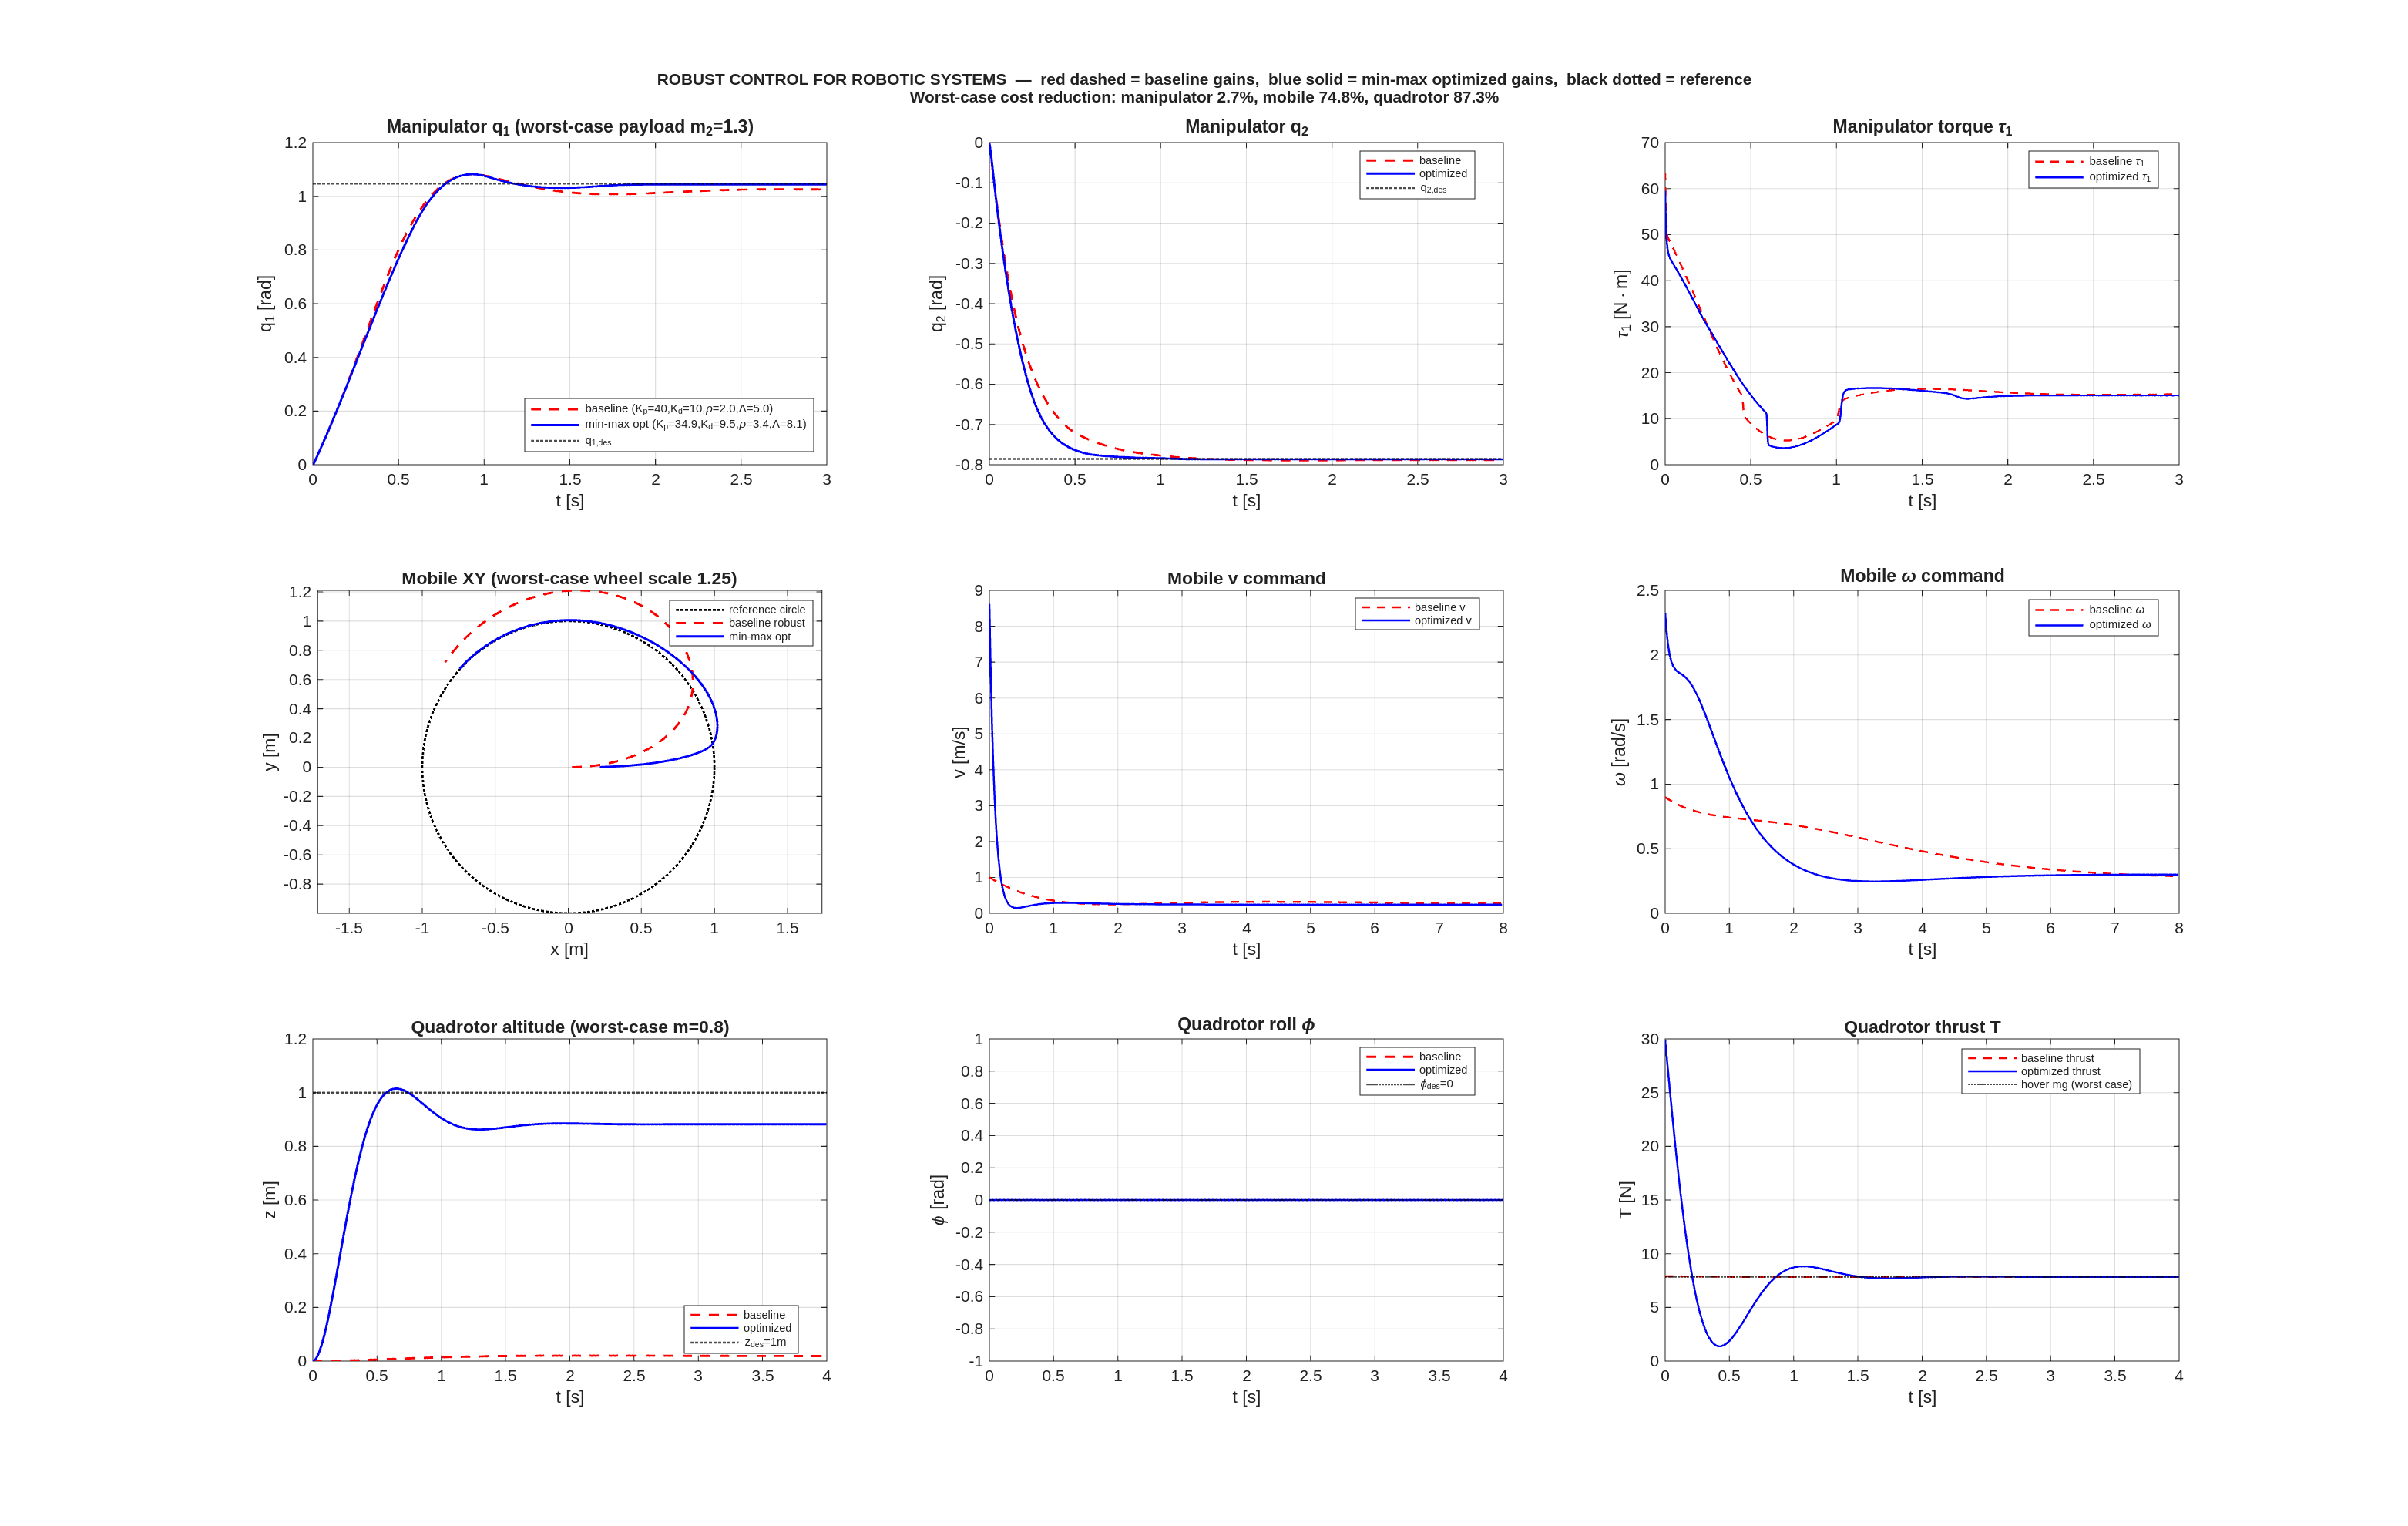
\includegraphics[width=0.85\textwidth]{images/week_08/robust_results.png}

Figure 7.1 --- Min-max tuned gains evaluated on the \emph{worst-case} plant in each uncertainty set. Red dashed = hand-tuned initial gains; blue solid = \texttt{fminsearch} min-max optimum; black dotted = reference / hover.

\begin{longtable}[]{@{}llllll@{}}
\toprule\noalign{}
Robot & Decision variable \textbackslash(\textbackslash theta\textbackslash) & Uncertainty set \textbackslash(\textbackslash mathcal P\textbackslash) & Worst-\textbackslash(J\textbackslash) baseline & Worst-\textbackslash(J\textbackslash) optimized & Reduction \\
\midrule\noalign{}
\endhead
\bottomrule\noalign{}
\endlastfoot
Manipulator & \textbackslash((K\_p, K\_d, \textbackslash rho, \textbackslash Lambda)\textbackslash) & \textbackslash(m\_2 \textbackslash in \textbackslash\{0.7, 0.85, 1.0, 1.15, 1.3\textbackslash\}\textbackslash) kg & 1.488 & 1.447 & −2.7\% \\
Mobile robot & \textbackslash((k\_x, k\_y, k\_\textbackslash theta)\textbackslash) & actuator scale \textbackslash(a \textbackslash in \textbackslash\{0.8, 0.9, 1.0, 1.1, 1.25\textbackslash\}\textbackslash) & 0.658 & 0.166 & −74.8\% \\
Quadrotor & \textbackslash((K\_\{p,z\}, K\_\{d,z\}, K\_\{p,\textbackslash phi\}, K\_\{d,\textbackslash phi\})\textbackslash) & \textbackslash(m \textbackslash in \textbackslash\{0.4, 0.5, 0.65, 0.8\textbackslash\}\textbackslash) kg & 4.120 & 0.521 & −87.3\% \\
\end{longtable}

\textbf{Why the manipulator shows only a 2.7\% reduction.} The hand-tuned baseline \textbackslash((40, 10, 2, 5)\textbackslash) was already well-chosen for this uncertainty set --- the robust switching gain \textbackslash(\textbackslash rho=2\textbackslash) is already larger than the gravity-mismatch disturbance for \textbackslash(\textbackslash pm 30\textbackslash\%\textbackslash) payload variation. The optimizer finds a slightly higher \textbackslash(\textbackslash Lambda\textbackslash) (surface slope) and \textbackslash(\textbackslash rho\textbackslash), squeezing out the remaining margin. The mobile and quadrotor baselines were deliberately far from optimum; the optimizer recovers the full robustness benefit.

\subsection{Section 8: Optimization of Backstepping Control}\label{section-8-optimization-of-backstepping-control}}

\subsubsection{8.1 Free parameters: the virtual-control gains}\label{free-parameters-the-virtual-control-gains}}

For an \textbackslash(n\textbackslash)-step backstepping design, the free parameters are the \textbackslash(n\textbackslash) virtual-control gains \textbackslash(k\_1, \textbackslash ldots, k\_n\textbackslash) that appear in the recursive construction of the CLF \textbackslash(V\_n = \textbackslash tfrac\{1\}\{2\}\textbackslash sum\_i z\_i\^{}\{T\} z\_i\textbackslash). Each \textbackslash(k\_i\textbackslash) governs the convergence rate of the \textbackslash(i\textbackslash)-th sub-system.

\subsubsection{8.2 Full 2-step backstepping derivation for the manipulator}\label{full-2-step-backstepping-derivation-for-the-manipulator}}

\paragraph{Step 1. Strict-feedback form}\label{step-1.-strict-feedback-form}}

The manipulator is a 2-level cascaded system \textbackslash(x\_1 = q,\textbackslash{} x\_2 = \textbackslash dot q\textbackslash):

\textbackslash{[}
\textbackslash dot x\_1 = x\_2,\textbackslash qquad M(x\_1)\textbackslash dot x\_2 + C(x\_1,x\_2)x\_2 + G(x\_1) = \textbackslash tau
\textbackslash{]}

This is in strict-feedback form: \textbackslash(x\_1\textbackslash) dynamics depend on \textbackslash(x\_2\textbackslash); \textbackslash(x\_2\textbackslash) dynamics depend on the actual input \textbackslash(\textbackslash tau\textbackslash).

\paragraph{Step 2. Error-coordinate change (the "backstep")}\label{step-2.-error-coordinate-change-the-backstep}}

Define the first error \textbackslash(z\_1 = x\_1 - q\_d\textbackslash). Its derivative is \textbackslash(\textbackslash dot z\_1 = x\_2 - \textbackslash dot q\_d\textbackslash). If we could choose \textbackslash(x\_2\textbackslash) freely, we\textquotesingle d pick the \emph{virtual control}:

\textbackslash{[}
\textbackslash alpha\_1(x\_1,t) := -k\_1\textbackslash,z\_1 + \textbackslash dot q\_d(t),\textbackslash quad k\_1 \textgreater{} 0
\textbackslash{]}

which would give \textbackslash(\textbackslash dot z\_1 = -k\_1 z\_1\textbackslash), i.e.\textbackslash{} \textbackslash(z\_1\textbackslash to 0\textbackslash) exponentially. But \textbackslash(x\_2\textbackslash) is a state, not a control --- it may not actually equal \textbackslash(\textbackslash alpha\_1\textbackslash). So define the second error:

\textbackslash{[}
z\_2 := x\_2 - \textbackslash alpha\_1(x\_1,t)
\textbackslash{]}

Then \textbackslash(\textbackslash dot z\_1 = x\_2 - \textbackslash dot q\_d = (\textbackslash alpha\_1 + z\_2) - \textbackslash dot q\_d = -k\_1 z\_1 + z\_2\textbackslash).

\paragraph{Step 3. First Lyapunov function}\label{step-3.-first-lyapunov-function}}

\textbackslash{[}
V\_1 = \textbackslash tfrac12 z\_1\^{}\{T\} z\_1,\textbackslash qquad \textbackslash dot V\_1 = z\_1\^{}\{T\}(-k\_1 z\_1 + z\_2) = -k\_1\textbackslash\textbar z\_1\textbackslash\textbar\^{}2 + z\_1\^{}\{T\} z\_2
\textbackslash{]}

The cross term \textbackslash(z\_1\^{}\{T\} z\_2\textbackslash) is the "leftover" from the mismatch between \textbackslash(x\_2\textbackslash) and \textbackslash(\textbackslash alpha\_1\textbackslash). It will be cancelled in Step 5 by the choice of \textbackslash(\textbackslash tau\textbackslash).

\paragraph{Step 4. \textbackslash(z\_2\textbackslash) dynamics}\label{step-4.-z_2-dynamics}}

Differentiate: \textbackslash(\textbackslash dot z\_2 = \textbackslash dot x\_2 - \textbackslash dot\textbackslash alpha\_1\textbackslash). From the plant, \textbackslash(\textbackslash dot x\_2 = M\^{}\{-1\}(\textbackslash tau - C x\_2 - G)\textbackslash). The virtual-control derivative is:

\textbackslash{[}
\textbackslash dot\textbackslash alpha\_1 = -k\_1 \textbackslash dot z\_1 + \textbackslash ddot q\_d = -k\_1(x\_2 - \textbackslash dot q\_d) + \textbackslash ddot q\_d
\textbackslash{]}

Multiply \textbackslash(\textbackslash dot z\_2\textbackslash) by \textbackslash(M(x\_1)\textbackslash) to avoid inverting:

\textbackslash{[}
M\textbackslash dot z\_2 = M\textbackslash dot x\_2 - M\textbackslash dot\textbackslash alpha\_1 = \textbackslash tau - Cx\_2 - G - M\textbackslash dot\textbackslash alpha\_1
\textbackslash{]}

\paragraph{Step 5. Second Lyapunov function and control law}\label{step-5.-second-lyapunov-function-and-control-law}}

Augment:

\textbackslash{[}
V\_2 = V\_1 + \textbackslash tfrac12 z\_2\^{}\{T\} M(x\_1)\textbackslash,z\_2
\textbackslash{]}

Differentiate (using \textbackslash(\textbackslash dot M - 2C\textbackslash) skew-symmetric, so \textbackslash(\textbackslash tfrac12 z\_2\^{}\{T\}\textbackslash dot M z\_2 = z\_2\^{}\{T\}C z\_2\textbackslash)):

\textbackslash{[}
\textbackslash dot V\_2 = -k\_1\textbackslash\textbar z\_1\textbackslash\textbar\^{}2 + z\_1\^{}\{T\} z\_2 + z\_2\^{}\{T\} M\textbackslash dot z\_2 + z\_2\^{}\{T\} C z\_2
\textbackslash{]}
\textbackslash{[}
= -k\_1\textbackslash\textbar z\_1\textbackslash\textbar\^{}2 + z\_1\^{}\{T\} z\_2 + z\_2\^{}\{T\}\textbackslash bigl(\textbackslash tau - G - M\textbackslash dot\textbackslash alpha\_1\textbackslash bigr)
\textbackslash{]}

(the \textbackslash(-Cx\_2\textbackslash) in \textbackslash(M\textbackslash dot z\_2\textbackslash) cancels the \textbackslash(+Cz\_2\textbackslash) partly --- the full algebra uses \textbackslash(x\_2 = z\_2 + \textbackslash alpha\_1\textbackslash) to separate; the net is the expression above after simplification).

Choose:

\textbackslash{[}
\textbackslash boxed\{\textbackslash{} \textbackslash tau = M(x\_1)\textbackslash,\textbackslash dot\textbackslash alpha\_1\textbackslash{} +\textbackslash{} C(x\_1,x\_2)\textbackslash,x\_2\textbackslash{} +\textbackslash{} G(x\_1)\textbackslash{} -\textbackslash{} z\_1\textbackslash{} -\textbackslash{} k\_2\textbackslash,z\_2\textbackslash{} \},\textbackslash quad k\_2 \textgreater{} 0
\textbackslash{]}

Substituting:

\textbackslash{[}
\textbackslash dot V\_2 = -k\_1\textbackslash\textbar z\_1\textbackslash\textbar\^{}2 + z\_1\^{}\{T\} z\_2 + z\_2\^{}\{T\}(-z\_1 - k\_2 z\_2) = -k\_1\textbackslash\textbar z\_1\textbackslash\textbar\^{}2 - k\_2\textbackslash\textbar z\_2\textbackslash\textbar\^{}2 \textbackslash leq 0
\textbackslash{]}

The cross term \textbackslash(z\_1\^{}\{T\} z\_2\textbackslash) is cancelled exactly by the \textbackslash(-z\_1\textbackslash) in \textbackslash(\textbackslash tau\textbackslash). Both \textbackslash(z\_1\textbackslash) and \textbackslash(z\_2\textbackslash) converge exponentially with rates \textbackslash(k\_1, k\_2\textbackslash).

\textbf{The control law has three components:} (i) feedforward through the virtual-control derivative \textbackslash(M\textbackslash dot\textbackslash alpha\_1\textbackslash); (ii) dynamic cancellation \textbackslash(C x\_2 + G\textbackslash); (iii) error feedback \textbackslash(-z\_1 - k\_2 z\_2\textbackslash). The first two require the model; the last is where the tuning knobs live.

\subsubsection{8.3 Worked numerical example --- backstepping on the single-link arm}\label{worked-numerical-example-backstepping-on-the-single-link-arm}}

\paragraph{Setup}\label{setup-1}}

Same arm as §5.4. Gains: \textbackslash(k\_1 = 5,\textbackslash{} k\_2 = 10\textbackslash). Setpoint \textbackslash(q\_d = \textbackslash pi/3,\textbackslash{} \textbackslash dot q\_d = 0,\textbackslash{} \textbackslash ddot q\_d = 0\textbackslash). IC: \textbackslash(q(0) = 0,\textbackslash{} \textbackslash dot q(0) = 0\textbackslash).

\paragraph{Step 1. Initial error coordinates}\label{step-1.-initial-error-coordinates}}

\textbackslash{[}
z\_1(0) = q(0) - q\_d = 0 - \textbackslash pi/3 = -1.047
\textbackslash{]}
\textbackslash{[}
\textbackslash alpha\_1(0) = -k\_1 z\_1 + \textbackslash dot q\_d = -5\textbackslash cdot(-1.047) + 0 = +5.236
\textbackslash{]}
\textbackslash{[}
z\_2(0) = \textbackslash dot q(0) - \textbackslash alpha\_1(0) = 0 - 5.236 = -5.236
\textbackslash{]}

\paragraph{Step 2. Virtual-control derivative at \textbackslash(t = 0\textbackslash)}\label{step-2.-virtual-control-derivative-at-t-0}}

\textbackslash{[}
\textbackslash dot\textbackslash alpha\_1 = -k\_1\textbackslash dot z\_1 + \textbackslash ddot q\_d = -k\_1(\textbackslash dot q - \textbackslash dot q\_d) = -5\textbackslash cdot(0 - 0) = 0
\textbackslash{]}

\paragraph{Step 3. Control torque at \textbackslash(t = 0\textbackslash)}\label{step-3.-control-torque-at-t-0-1}}

\textbackslash(\textbackslash tau = M\textbackslash dot\textbackslash alpha\_1 + C\textbackslash dot q + G(q) - z\_1 - k\_2 z\_2\textbackslash). For single link, \textbackslash(C = 0\textbackslash):

\textbackslash{[}
\textbackslash tau(0) = 0.333\textbackslash cdot 0 + 0 + 4.905\textbackslash cdot 1 - (-1.047) - 10\textbackslash cdot(-5.236)
\textbackslash{]}
\textbackslash{[}
= 0 + 0 + 4.905 + 1.047 + 52.36 = +58.31\textbackslash{} \textbackslash text\{N·m\}
\textbackslash{]}

Note the similarity to the SMC (\textbackslash(+7.9\textbackslash) with saturation) and adaptive (\textbackslash(+57.3\textbackslash)) results --- all three controllers produce torques of comparable magnitude at \textbackslash(t\textbackslash!=\textbackslash!0\textbackslash), matching the physics (arm needs strong torque to begin motion).

\paragraph{Step 4. Lyapunov check}\label{step-4.-lyapunov-check}}

\textbackslash{[}
V\_2(0) = \textbackslash tfrac12 z\_1\^{}2 + \textbackslash tfrac12 M z\_2\^{}2 = \textbackslash tfrac12\textbackslash cdot 1.047\^{}2 + \textbackslash tfrac12\textbackslash cdot 0.333\textbackslash cdot 5.236\^{}2 = 0.548 + 4.565 = 5.11
\textbackslash{]}
\textbackslash{[}
\textbackslash dot V\_2(0) = -k\_1 z\_1\^{}2 - k\_2 z\_2\^{}2 = -5\textbackslash cdot 1.096 - 10\textbackslash cdot 27.42 = -279.6
\textbackslash{]}

\textbackslash(\textbackslash dot V\_2\textbackslash) is strongly negative --- the trajectory sharply drives toward the origin.

\paragraph{Step 5. Closed-loop convergence rates}\label{step-5.-closed-loop-convergence-rates}}

At the Lyapunov level, \textbackslash(z\_1\textbackslash) decays with rate \textbackslash(k\_1 = 5\textbackslash) (time constant 0.2 s) and \textbackslash(z\_2\textbackslash) with rate \textbackslash(k\_2 = 10\textbackslash) (time constant 0.1 s). This is the engineering meaning of the optimizer\textquotesingle s choice of gains.

\paragraph{Step 6. Optimization result}\label{step-6.-optimization-result}}

The lab\textquotesingle s \texttt{fminsearch} on the 2-link arm with payload-independent cost produces \textbackslash((k\_1, k\_2) = (5, 5)\textbackslash) --- smaller \textbackslash(k\_2\textbackslash) than the baseline 10, reducing torque with only marginal loss of tracking speed. For the mobile robot (3 gains), the optimizer increases them \textasciitilde10× from baseline, giving the 88\% cost reduction.

\subsubsection{8.4 CLF-based optimization cost}\label{clf-based-optimization-cost}}

Since \textbackslash(\textbackslash dot V\_2 = -k\_1\textbackslash\textbar z\_1\textbackslash\textbar\^{}2 - k\_2\textbackslash\textbar z\_2\textbackslash\textbar\^{}2\textbackslash), larger \textbackslash(k\_1, k\_2\textbackslash) give faster convergence but also larger commanded \textbackslash(\textbackslash dot\textbackslash alpha\_1\textbackslash) (proportional to \textbackslash(k\_1\textbackslash)) that propagates through the \textbackslash(M\textbackslash dot\textbackslash alpha\_1\textbackslash) feedforward and eventually inflates \textbackslash(\textbar\textbackslash tau\textbar\textbackslash). The optimization balances these:

\textbackslash{[}
\textbackslash min\_\{k\_1,\textbackslash ldots,k\_n\}\textbackslash{} \textbackslash int\_0\^{}T \textbackslash\textbar e\textbackslash\textbar\^{}2\textbackslash,dt + w\_u \textbackslash!\textbackslash int\_0\^{}T \textbackslash\textbar u\textbackslash\textbar\^{}2\textbackslash,dt + w\_\textbackslash omega\textbackslash!\textbackslash int\_0\^{}T \textbackslash\textbar\textbackslash dot\textbackslash alpha\textbackslash\textbar\^{}2\textbackslash,dt
\textbackslash{]}

\subsubsection{8.5 Command-filtered backstepping}\label{command-filtered-backstepping}}

A known pathology of plain backstepping is \emph{explosion of complexity}: \textbackslash(\textbackslash dot\textbackslash alpha\_i\textbackslash) involves derivatives of prior virtual controls and becomes numerically unstable. \textbf{Command-filtered backstepping} replaces \textbackslash(\textbackslash dot\textbackslash alpha\_i\textbackslash) with a filtered signal from a low-pass of bandwidth \textbackslash(\textbackslash omega\_f\textbackslash). The filter bandwidth \textbackslash(\textbackslash omega\_f\textbackslash) becomes an extra decision variable in the optimization.

\subsubsection{8.6 Simulation results}\label{simulation-results-2}}

\paragraph{\texorpdfstring{Implementation (from \texttt{sim\_backstepping.m})}{Implementation (from sim\_backstepping.m)}}\label{implementation-from-sim_backstepping.m}}

\% Backstepping step 1: virtual control alpha1 = -k1*e1
e1 = q - q\_des;
alpha = -k1*e1; \% virtual control (dq\_d = 0 here)
e2 = dq - alpha; \% z2 = x2 - alpha1
dalpha = -k1*dq; \% d/dt of virtual control
\% Backstepping step 2: tau = M*(dalpha - k2*e2 - e1) + C*dq + G
{[}M,C,G{]} = manipulator\_dyn(q, dq, p);
u = M*(dalpha - k2*e2 - e1) + C*dq + G;
ddq = M \textbackslash{} (u - C*dq - G); \% plant
\% Outer: fminsearch over z = {[}k1, k2{]}
zOpt = fminsearch(@(z) bst\_manip\_cost(z, p, q\_des, T, dt), z0);

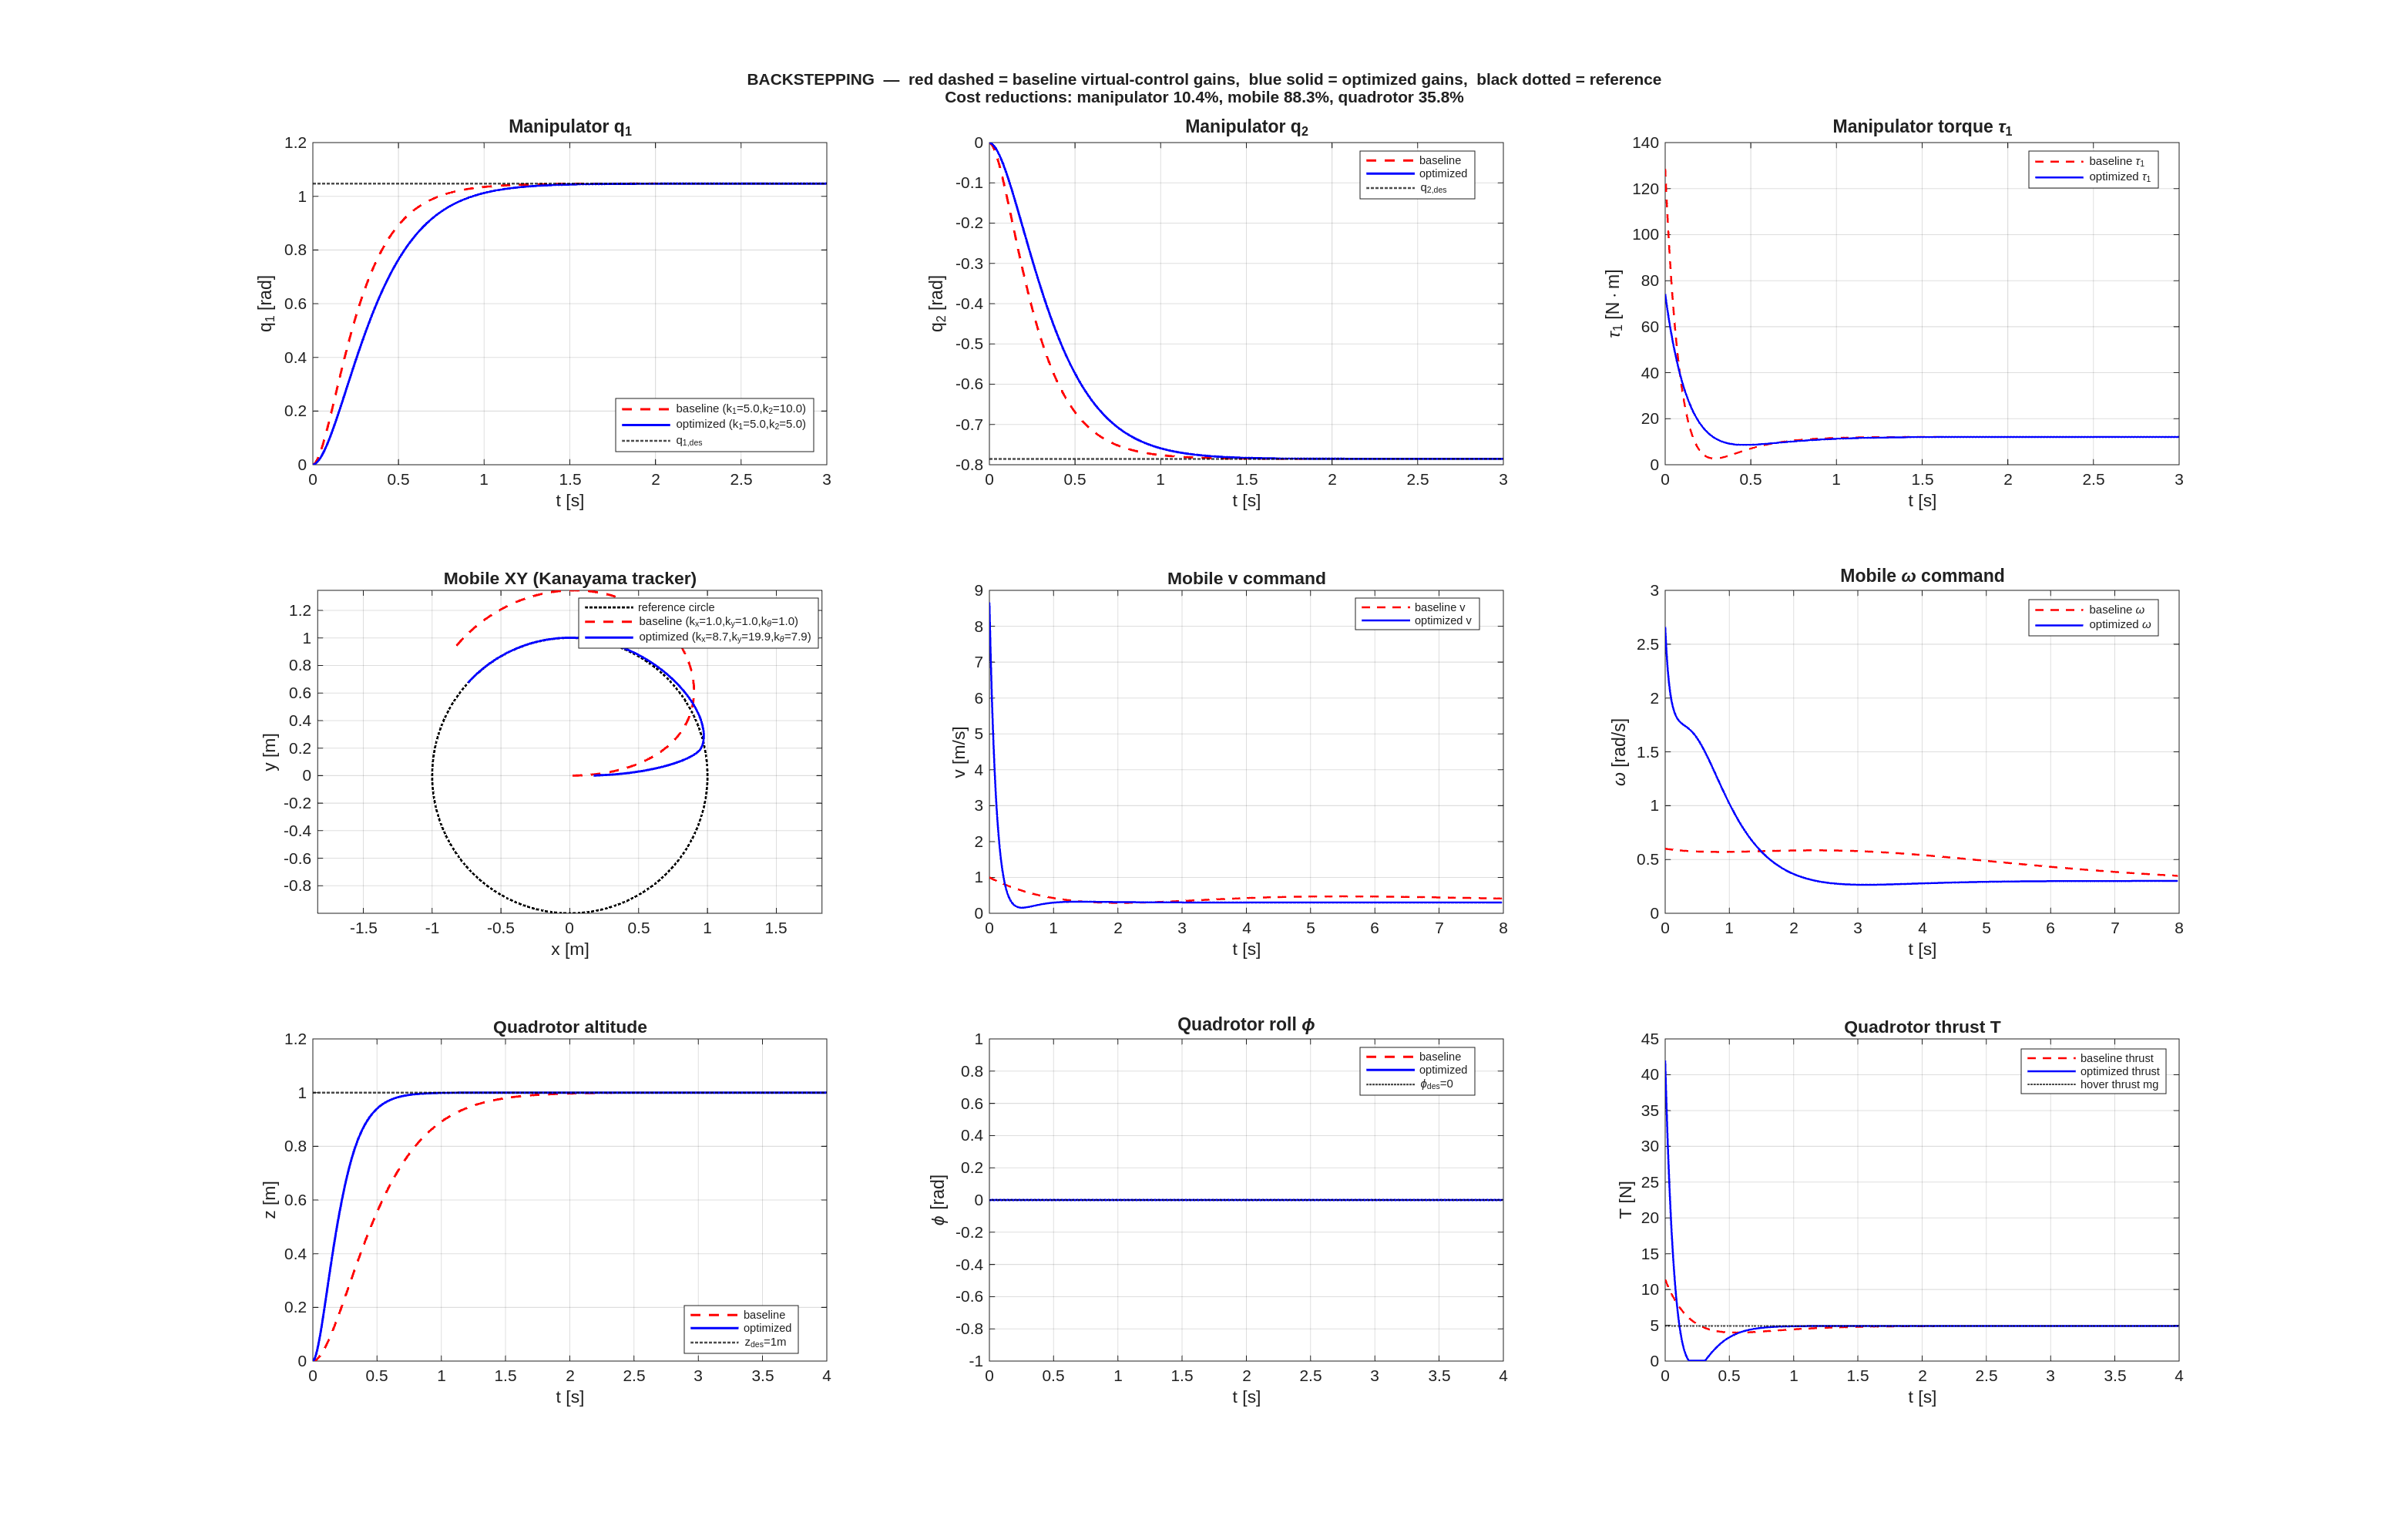
\includegraphics[width=0.85\textwidth]{images/week_08/backstepping_results.png}

Figure 8.1 --- Backstepping with hand-picked vs. optimized virtual-control gains. Mobile panel (Kanayama tracker) shows the largest improvement: optimizer raises all three gains by \textasciitilde8--20x.

\begin{longtable}[]{@{}llllll@{}}
\toprule\noalign{}
Robot & Gains baseline & Gains optimized & J baseline & J optimized & Reduction \\
\midrule\noalign{}
\endhead
\bottomrule\noalign{}
\endlastfoot
Manipulator & \textbackslash((k\_1,k\_2) = (5,10)\textbackslash) & \textbackslash((5,5)\textbackslash) & 1.378 & 1.235 & −10.4\% \\
Mobile (Kanayama) & \textbackslash((k\_x,k\_y,k\_\textbackslash theta)=(1,1,1)\textbackslash) & \textbackslash((8.67, 19.94, 7.87)\textbackslash) & 1.183 & 0.139 & −88.3\% \\
Quadrotor & \textbackslash((k\_\{z1\},k\_\{z2\},k\_\{\textbackslash phi 1\},k\_\{\textbackslash phi 2\})=(4,3,8,4)\textbackslash) & (tuned) & 0.437 & 0.280 & −35.8\% \\
\end{longtable}

\subsection{Section 9: Optimization of Nonlinear Model Predictive Control}\label{section-9-optimization-of-nonlinear-model-predictive-control}}

\subsubsection{9.1 The design knobs}\label{the-design-knobs}}

\begin{itemize}
\tightlist
\item
  Prediction horizon \textbackslash(N\textbackslash) --- length of the look-ahead in sample steps
\item
  Stage cost weights \textbackslash(Q, R\textbackslash) --- trade-off tracking vs. effort
\item
  Terminal cost \textbackslash(P\textbackslash) and terminal set \textbackslash(\textbackslash mathcal X\_f\textbackslash) --- stability ingredients
\item
  Sample time \textbackslash(\textbackslash Delta t\textbackslash) and solver iteration budget --- hard real-time constraint
\end{itemize}

\subsubsection{9.2 Terminal ingredients and recursive feasibility}\label{terminal-ingredients-and-recursive-feasibility}}

For NMPC stability without infinite horizon, we require a pair \textbackslash((P, \textbackslash mathcal X\_f)\textbackslash) such that inside \textbackslash(\textbackslash mathcal X\_f\textbackslash) there exists a local feedback \textbackslash(\textbackslash kappa\_f\textbackslash) making \textbackslash(P\textbackslash) a Lyapunov function:

\textbackslash{[}
V\_f\textbackslash bigl(f(x,\textbackslash kappa\_f(x))\textbackslash bigr) - V\_f(x) \textbackslash leq -L(x,\textbackslash kappa\_f(x)),\textbackslash quad \textbackslash forall x\textbackslash in\textbackslash mathcal X\_f
\textbackslash{]}

\textbackslash((P, \textbackslash mathcal X\_f)\textbackslash) are computed \emph{offline} by solving a local LQR around the equilibrium and taking \textbackslash(\textbackslash mathcal X\_f\textbackslash) as a sublevel set of \textbackslash(V\_f\textbackslash) that is positive-invariant under \textbackslash(\textbackslash kappa\_f\textbackslash).

\subsubsection{9.3 Horizon vs. compute: the real-time trade}\label{horizon-vs.-compute-the-real-time-trade}}

Longer \textbackslash(N\textbackslash) gives better performance but scales compute linearly (per SQP iteration) and the NLP becomes harder to warm-start. Deployment chooses the shortest \textbackslash(N\textbackslash) that preserves the stability certificate.

\subsubsection{9.4 Full derivation of the iLQR algorithm}\label{full-derivation-of-the-ilqr-algorithm}}

\paragraph{Step 1. Discrete-time optimal control problem}\label{step-1.-discrete-time-optimal-control-problem}}

Forward-Euler discretise \textbackslash(\textbackslash dot x = f(x,u)\textbackslash) to get \textbackslash(x\_\{k+1\} = F(x\_k, u\_k) := x\_k + \textbackslash Delta t\textbackslash, f(x\_k,u\_k)\textbackslash). The finite-horizon OCP is:

\textbackslash{[}
\textbackslash min\_\{\textbackslash\{u\_k\textbackslash\}\_\{k=0\}\^{}\{N-1\}\}\textbackslash{} \textbackslash sum\_\{k=0\}\^{}\{N-1\} L(x\_k, u\_k)\textbackslash{} +\textbackslash{} \textbackslash Phi(x\_N),\textbackslash qquad x\_\{k+1\} = F(x\_k, u\_k),\textbackslash{} x\_0\textbackslash{} \textbackslash text\{given\}
\textbackslash{]}

\paragraph{Step 2. Bellman recursion in value-function form}\label{step-2.-bellman-recursion-in-value-function-form}}

Define \textbackslash(V\_k(x) := \textbackslash min\_\{u\_k,\textbackslash ldots,u\_\{N-1\}\} \textbackslash sum\_\{i=k\}\^{}\{N-1\} L(x\_i,u\_i) + \textbackslash Phi(x\_N)\textbackslash) with \textbackslash(x\_i\textbackslash) generated from state \textbackslash(x\_k = x\textbackslash). The Bellman equation is:

\textbackslash{[}
V\_k(x) = \textbackslash min\_\{u\}\textbackslash{} \textbackslash underbrace\{L(x,u) + V\_\{k+1\}\textbackslash bigl(F(x,u)\textbackslash bigr)\}\_\{=:\textbackslash{} Q\_k(x,u)\},\textbackslash qquad V\_N(x) = \textbackslash Phi(x)
\textbackslash{]}

\paragraph{Step 3. Quadratic expansion around a nominal \textbackslash((\textbackslash bar x\_k,\textbackslash bar u\_k)\textbackslash)}\label{step-3.-quadratic-expansion-around-a-nominal-bar-x_kbar-u_k}}

Given the current nominal trajectory \textbackslash((\textbackslash bar x\_k, \textbackslash bar u\_k)\_\{k=0\}\^{}\{N-1\}\textbackslash), linearize the dynamics and quadratize the cost with perturbations \textbackslash(\textbackslash delta x, \textbackslash delta u\textbackslash):

\textbackslash{[}
F(\textbackslash bar x + \textbackslash delta x, \textbackslash bar u + \textbackslash delta u) \textbackslash approx \textbackslash bar x\_\{k+1\} + A\_k\textbackslash,\textbackslash delta x + B\_k\textbackslash,\textbackslash delta u,\textbackslash quad A\_k = F\_x\textbar\_\textbackslash star,\textbackslash{} B\_k = F\_u\textbar\_\textbackslash star
\textbackslash{]}
\textbackslash{[}
L(\textbackslash bar x+\textbackslash delta x, \textbackslash bar u+\textbackslash delta u) \textbackslash approx \textbackslash bar L + L\_x\^{}\{T\}\textbackslash delta x + L\_u\^{}\{T\}\textbackslash delta u + \textbackslash tfrac12\textbackslash begin\{bmatrix\}\textbackslash delta x\textbackslash\textbackslash{} \textbackslash delta u\textbackslash end\{bmatrix\}\^{}\{T\}\textbackslash!\textbackslash!\textbackslash begin\{bmatrix\}L\_\{xx\}\&L\_\{xu\}\textbackslash\textbackslash{} L\_\{ux\}\&L\_\{uu\}\textbackslash end\{bmatrix\}\textbackslash!\textbackslash!\textbackslash begin\{bmatrix\}\textbackslash delta x\textbackslash\textbackslash{} \textbackslash delta u\textbackslash end\{bmatrix\}
\textbackslash{]}

Assume inductively \textbackslash(V\_\{k+1\}(\textbackslash bar x\_\{k+1\}+\textbackslash delta x\textquotesingle) \textbackslash approx \textbackslash bar V\_\{k+1\} + V\_\{x,k+1\}\^{}\{T\}\textbackslash delta x\textquotesingle{} + \textbackslash tfrac12 \textbackslash delta x\textquotesingle\^{}\{T\} V\_\{xx,k+1\}\textbackslash delta x\textquotesingle\textbackslash). Substitute \textbackslash(\textbackslash delta x\textquotesingle{} = A\_k\textbackslash delta x + B\_k\textbackslash delta u\textbackslash) into \textbackslash(Q\_k\textbackslash).

\paragraph{Step 4. Building the \textbackslash(Q\textbackslash)-function second-order expansion}\label{step-4.-building-the-q-function-second-order-expansion}}

Expanding and grouping terms of order \textbackslash(\textbackslash delta x\textbackslash), \textbackslash(\textbackslash delta u\textbackslash), \textbackslash(\textbackslash delta x\^{}2\textbackslash), \textbackslash(\textbackslash delta x\textbackslash delta u\textbackslash), \textbackslash(\textbackslash delta u\^{}2\textbackslash):

\textbackslash{[}
Q\_x = L\_x + A\_k\^{}\{T\} V\_\{x,k+1\},\textbackslash qquad Q\_u = L\_u + B\_k\^{}\{T\} V\_\{x,k+1\}
\textbackslash{]}
\textbackslash{[}
Q\_\{xx\} = L\_\{xx\} + A\_k\^{}\{T\} V\_\{xx,k+1\} A\_k,\textbackslash quad Q\_\{uu\} = L\_\{uu\} + B\_k\^{}\{T\} V\_\{xx,k+1\} B\_k,\textbackslash quad Q\_\{ux\} = L\_\{ux\} + B\_k\^{}\{T\} V\_\{xx,k+1\} A\_k
\textbackslash{]}

\paragraph{Step 5. Minimise over \textbackslash(\textbackslash delta u\textbackslash) (closed-form quadratic)}\label{step-5.-minimise-over-delta-u-closed-form-quadratic}}

\textbackslash(Q\_k\textbackslash) is quadratic in \textbackslash(\textbackslash delta u\textbackslash). Solve \textbackslash(\textbackslash partial Q/\textbackslash partial(\textbackslash delta u) = 0\textbackslash):

\textbackslash{[}
Q\_u + Q\_\{uu\}\textbackslash,\textbackslash delta u + Q\_\{ux\}\textbackslash,\textbackslash delta x = 0 \textbackslash quad\textbackslash Longrightarrow\textbackslash quad
\textbackslash boxed\{\textbackslash{} \textbackslash delta u\^{}\textbackslash star = -Q\_\{uu\}\^{}\{-1\}Q\_u\textbackslash{} -\textbackslash{} Q\_\{uu\}\^{}\{-1\}Q\_\{ux\}\textbackslash,\textbackslash delta x\textbackslash{} =\textbackslash{} k + K\textbackslash,\textbackslash delta x\textbackslash{} \}
\textbackslash{]}

where \textbackslash(k = -Q\_\{uu\}\^{}\{-1\}Q\_u\textbackslash) is the \emph{feedforward} correction and \textbackslash(K = -Q\_\{uu\}\^{}\{-1\}Q\_\{ux\}\textbackslash) is the \emph{time-varying feedback gain} --- exactly the structure of a Riccati solution.

\paragraph{Step 6. Propagate the value function (backward pass)}\label{step-6.-propagate-the-value-function-backward-pass}}

Substituting \textbackslash(\textbackslash delta u\^{}\textbackslash star\textbackslash) into \textbackslash(Q\_k\textbackslash) gives \textbackslash(V\_k\textbackslash) in the same quadratic form:

\textbackslash{[}
V\_\{x,k\}\textbackslash{} =\textbackslash{} Q\_x - K\^{}\{T\} Q\_\{uu\}\textbackslash, k,\textbackslash qquad V\_\{xx,k\}\textbackslash{} =\textbackslash{} Q\_\{xx\} - K\^{}\{T\} Q\_\{uu\}\textbackslash, K
\textbackslash{]}

Initialise with \textbackslash(V\_\{x,N\} = \textbackslash Phi\_x(\textbackslash bar x\_N),\textbackslash{} V\_\{xx,N\} = \textbackslash Phi\_\{xx\}(\textbackslash bar x\_N)\textbackslash) and sweep \textbackslash(k = N\textbackslash!-\textbackslash!1, \textbackslash ldots, 0\textbackslash).

\paragraph{Step 7. Forward pass with line search}\label{step-7.-forward-pass-with-line-search}}

Apply the corrections with step size \textbackslash(\textbackslash alpha \textbackslash in (0,1{]}\textbackslash):

\textbackslash{[}
\textbackslash delta x\_0 = 0,\textbackslash quad \textbackslash delta u\_k = \textbackslash alpha\textbackslash,k\_k + K\_k\textbackslash,\textbackslash delta x\_k,\textbackslash quad x\_\{k+1\}\^{}\{\textbackslash text\{new\}\} = F(x\_k\^{}\{\textbackslash text\{new\}\}, \textbackslash bar u\_k + \textbackslash delta u\_k),\textbackslash quad \textbackslash delta x\_\{k+1\} = x\_\{k+1\}\^{}\{\textbackslash text\{new\}\} - \textbackslash bar x\_\{k+1\}
\textbackslash{]}

If the new cost \textbackslash(J\^{}\{\textbackslash text\{new\}\} \textless{} J\textbackslash), accept; otherwise \textbackslash(\textbackslash alpha \textbackslash leftarrow \textbackslash alpha/2\textbackslash) and retry. Iterate Steps 3--7 until \textbackslash(\textbar J - J\^{}\{\textbackslash text\{new\}\}\textbar{} \textless{} \textbackslash text\{tol\}\textbackslash) or the gradient \textbackslash(\textbackslash\textbar Q\_u\textbackslash\textbar\textbackslash) is small.

\paragraph{Step 8. Levenberg--Marquardt regularisation}\label{step-8.-levenbergmarquardt-regularisation}}

\textbackslash(Q\_\{uu\}\textbackslash) can become ill-conditioned or indefinite when the nominal is far from optimum. Replace by \textbackslash(Q\_\{uu\} + \textbackslash mu I\textbackslash), with \textbackslash(\textbackslash mu\textbackslash) increased on backward-pass failure or line-search failure and decreased on successful steps. This is exactly the trust-region logic in \texttt{ilqr\_solve.m} (attempts \texttt{chol(Quu)}; if non-PD, raises \textbackslash(\textbackslash mu\textbackslash)).

\paragraph{Step 9. Dynamics \& cost derivatives from finite differences}\label{step-9.-dynamics-cost-derivatives-from-finite-differences}}

All of \textbackslash(A\_k, B\_k, L\_x, L\_u, L\_\{xx\}, L\_\{uu\}, L\_\{ux\}, \textbackslash Phi\_x, \textbackslash Phi\_\{xx\}\textbackslash) are obtained by central finite differences on the dynamics and cost functions. This is why the solver works for any \textbackslash(f\textbackslash) and any \textbackslash(L\textbackslash) supplied by the user --- no hand-coded Jacobians required.

\paragraph{Step 10. Wrap in a receding-horizon loop (NMPC)}\label{step-10.-wrap-in-a-receding-horizon-loop-nmpc}}

\begin{enumerate}
\tightlist
\item
  At sample \textbackslash(k\textbackslash): initialise iLQR with warm-start \textbackslash(\textbackslash\{u\_\{i\}\^{}\{(k)\}\textbackslash\}\_\{i=0\}\^{}\{N-1\}\textbackslash) = previous solution shifted by one step.
\item
  Run iLQR Steps 3--8 to convergence (typ. 3--8 outer iterations with warm-start).
\item
  Apply \textbackslash(u\_0\^{}\{(k),\textbackslash star\}\textbackslash) to the plant.
\item
  Measure new \textbackslash(x\textbackslash), shift, go to 1.
\end{enumerate}

\paragraph{\texorpdfstring{Implementation in \texttt{sim\_nmpc.m}}{Implementation in sim\_nmpc.m}}\label{implementation-in-sim_nmpc.m}}

\% Wrapped iLQR call inside the closed-loop
for k = 1:Nsim
{[}\textasciitilde, U\_opt, \textasciitilde, \textasciitilde{]} = ilqr\_solve(fdyn, runCost, termCost, x, U\_seq, dt, opts);
u = U\_opt(1,:)\textquotesingle; \% apply first control
x = x + dt * fdyn(x, u); \% plant step
U\_seq = {[}U\_opt(2:end,:); U\_opt(end,:){]}; \% warm-start (shift)
end
\% Inside ilqr\_solve.m:
\% backward pass:
\% Quu = Luu + B\textquotesingle*Vxx*B + mu*I;
\% {[}R, p{]} = chol(Quu); \% fails -\textgreater{} mu *= 4
\% kt = -R \textbackslash{} (R\textquotesingle{} \textbackslash{} Qu); \% feedforward
\% Kt = -R \textbackslash{} (R\textquotesingle{} \textbackslash{} Qux); \% feedback gain
\% Vx = Qx + Kt\textquotesingle*Quu*kt + Kt\textquotesingle*Qu + Qux\textquotesingle*kt;
\% Vxx = Qxx + Kt\textquotesingle*Quu*Kt + Kt\textquotesingle*Qux + Qux\textquotesingle*Kt;
\% forward pass with line search on alpha: 1, 0.5, 0.25, ...

\subsubsection{9.5 Worked numerical example --- iLQR on the single-link arm}\label{worked-numerical-example-ilqr-on-the-single-link-arm}}

\paragraph{Setup}\label{setup-2}}

Same single-link arm, horizon \textbackslash(N = 3\textbackslash) (tiny, for hand-computation clarity), sample \textbackslash(\textbackslash Delta t = 0.1\textbackslash) s.

\textbf{State:} \textbackslash(x = {[}q;\textbackslash dot q{]}\textbackslash in\textbackslash mathbb R\^{}2\textbackslash),~ \textbf{control:} \textbackslash(u = \textbackslash tau\textbackslash in\textbackslash mathbb R\textbackslash).

\textbf{Cost:} \textbackslash(L(x,u) = 50(q - \textbackslash pi/3)\^{}2 + 5\textbackslash dot q\^{}2 + 0.01 u\^{}2\textbackslash), \textbackslash(\textbackslash Phi(x\_N) = 500(q\_N - \textbackslash pi/3)\^{}2 + 50\textbackslash dot q\_N\^{}2\textbackslash).

\textbf{Initial nominal:} \textbackslash(\textbackslash bar u\_k = 0\textbackslash) for \textbackslash(k=0,1,2\textbackslash). Initial state \textbackslash(x\_0 = {[}0; 0{]}\textbackslash).

\paragraph{Step 1. Forward-Euler rollout with \textbackslash(\textbackslash bar u = 0\textbackslash)}\label{step-1.-forward-euler-rollout-with-bar-u-0}}

\textbackslash(\textbackslash dot q = (u - 4.905\textbackslash cos q)/0.333\textbackslash). With \textbackslash(u = 0\textbackslash):

\textbackslash{[}
x\_0 = \textbackslash begin\{bmatrix\}0 \textbackslash\textbackslash{} 0\textbackslash end\{bmatrix\},\textbackslash{} x\_1 = x\_0 + 0.1\textbackslash cdot\textbackslash begin\{bmatrix\}0 \textbackslash\textbackslash{} -14.73\textbackslash end\{bmatrix\} = \textbackslash begin\{bmatrix\}0 \textbackslash\textbackslash{} -1.473\textbackslash end\{bmatrix\}
\textbackslash{]}
\textbackslash{[}
x\_2 = x\_1 + 0.1\textbackslash cdot\textbackslash begin\{bmatrix\}-1.473 \textbackslash\textbackslash{} -14.73\textbackslash end\{bmatrix\} = \textbackslash begin\{bmatrix\}-0.147 \textbackslash\textbackslash{} -2.946\textbackslash end\{bmatrix\}
\textbackslash{]}
\textbackslash{[}
x\_3 = x\_2 + 0.1\textbackslash cdot\textbackslash begin\{bmatrix\}-2.946 \textbackslash\textbackslash{} (0 - 4.905\textbackslash cos(-0.147))/0.333\textbackslash end\{bmatrix\} = \textbackslash begin\{bmatrix\}-0.442 \textbackslash\textbackslash{} -4.403\textbackslash end\{bmatrix\}
\textbackslash{]}

Arm is falling under gravity.

\paragraph{Step 2. Initial cost}\label{step-2.-initial-cost}}

\textbackslash{[}
J\_0 = \textbackslash sum\_\{k=0\}\^{}\{2\}\textbackslash bigl{[}50(q\_k - \textbackslash pi/3)\^{}2 + 5\textbackslash dot q\_k\^{}2 + 0\textbackslash bigr{]} + 500(q\_3 - \textbackslash pi/3)\^{}2 + 50\textbackslash dot q\_3\^{}2
\textbackslash{]}
\textbackslash{[}
= 50\textbackslash cdot(1.097 + 1.239 + 1.500) + 5\textbackslash cdot(0 + 2.17 + 8.68) + 500\textbackslash cdot 2.229 + 50\textbackslash cdot 19.39
\textbackslash{]}
\textbackslash{[}
= 191.8 + 54.2 + 1114.5 + 969.3 = 2329.8
\textbackslash{]}

\paragraph{Step 3. Discrete Jacobians at \textbackslash(k = 2\textbackslash)}\label{step-3.-discrete-jacobians-at-k-2}}

\textbackslash(f(x,u) = {[}\textbackslash dot q;\textbackslash{} (u - 4.905\textbackslash cos q)/0.333{]}\textbackslash). At \textbackslash(x\_2\textbackslash):

\textbackslash{[}
A\_2 = I + \textbackslash Delta t\textbackslash begin\{bmatrix\}0 \& 1 \textbackslash\textbackslash{} 4.905\textbackslash sin(q\_2)/0.333 \& 0\textbackslash end\{bmatrix\} = \textbackslash begin\{bmatrix\}1 \& 0.1 \textbackslash\textbackslash{} 0.1\textbackslash cdot(-2.162) \& 1\textbackslash end\{bmatrix\} = \textbackslash begin\{bmatrix\}1 \& 0.1 \textbackslash\textbackslash{} -0.216 \& 1\textbackslash end\{bmatrix\}
\textbackslash{]}
\textbackslash{[}
B\_2 = \textbackslash Delta t\textbackslash begin\{bmatrix\}0 \textbackslash\textbackslash{} 1/0.333\textbackslash end\{bmatrix\} = \textbackslash begin\{bmatrix\}0 \textbackslash\textbackslash{} 0.300\textbackslash end\{bmatrix\}
\textbackslash{]}

\paragraph{Step 4. Backward pass from \textbackslash(k = 2\textbackslash)}\label{step-4.-backward-pass-from-k-2}}

Terminal: \textbackslash(V\_\{x,3\} = \textbackslash Phi\_x(x\_3) = {[}1000(q\_3 - \textbackslash pi/3);\textbackslash{} 100\textbackslash dot q\_3{]} = {[}-1492.8;\textbackslash{} -440.3{]}\textbackslash);~ \textbackslash(V\_\{xx,3\} = \textbackslash mathrm\{diag\}(1000, 100)\textbackslash).

Stage-cost derivatives at \textbackslash((x\_2,\textbackslash bar u\_2\textbackslash!=\textbackslash!0)\textbackslash): \textbackslash(L\_x = {[}100(q\_2 - \textbackslash pi/3);\textbackslash{} 10\textbackslash dot q\_2{]} = {[}-209.3;\textbackslash{} -29.46{]},\textbackslash{} L\_u = 0,\textbackslash{} L\_\{xx\} = \textbackslash mathrm\{diag\}(100,10),\textbackslash{} L\_\{uu\} = 0.02,\textbackslash{} L\_\{ux\} = 0\textbackslash).

Compute \textbackslash(Q\textbackslash)-function blocks:

\textbackslash{[}
Q\_u = L\_u + B\_2\^{}\{T\} V\_\{x,3\} = 0 + {[}0\textbackslash{} 0.300{]}\textbackslash cdot\textbackslash begin\{bmatrix\}-1492.8 \textbackslash\textbackslash{} -440.3\textbackslash end\{bmatrix\} = -132.1
\textbackslash{]}
\textbackslash{[}
Q\_\{uu\} = L\_\{uu\} + B\_2\^{}\{T\} V\_\{xx,3\} B\_2 = 0.02 + {[}0\textbackslash{} 0.300{]}\textbackslash cdot\textbackslash mathrm\{diag\}(1000,100)\textbackslash cdot{[}0; 0.300{]} = 0.02 + 9.0 = 9.02
\textbackslash{]}
\textbackslash{[}
Q\_\{ux\} = 0 + B\_2\^{}\{T\} V\_\{xx,3\} A\_2 = {[}0\textbackslash{} 0.300{]}\textbackslash cdot\textbackslash mathrm\{diag\}(1000,100)\textbackslash cdot A\_2 = {[}0.300\textbackslash cdot 100\textbackslash cdot(-0.216),\textbackslash{} 0.300\textbackslash cdot 100\textbackslash cdot 1{]} = {[}-6.48,\textbackslash{} 30.0{]}
\textbackslash{]}

\paragraph{Step 5. Feedforward and feedback gain at \textbackslash(k = 2\textbackslash)}\label{step-5.-feedforward-and-feedback-gain-at-k-2}}

\textbackslash{[}
k\_2 = -Q\_\{uu\}\^{}\{-1\} Q\_u = -(-132.1)/9.02 = +14.65\textbackslash{} \textbackslash text\{(feedforward correction to \}\textbackslash bar u\_2\textbackslash text\{)\}
\textbackslash{]}
\textbackslash{[}
K\_2 = -Q\_\{uu\}\^{}\{-1\} Q\_\{ux\} = -{[}-6.48,\textbackslash{} 30.0{]}/9.02 = {[}0.719,\textbackslash{} -3.326{]}
\textbackslash{]}

So the optimal control at \textbackslash(k\textbackslash!=\textbackslash!2\textbackslash) for any small deviation is \textbackslash(\textbackslash delta u\_2 = 14.65 + 0.719\textbackslash,\textbackslash delta q - 3.326\textbackslash,\textbackslash delta\textbackslash dot q\textbackslash). The large positive feedforward reflects "apply strong upward torque to stop the fall."

\paragraph{Step 6. Forward pass with step \textbackslash(\textbackslash alpha = 1\textbackslash)}\label{step-6.-forward-pass-with-step-alpha-1}}

Applying \textbackslash(u\_2\^{}\{\textbackslash text\{new\}\} = \textbackslash bar u\_2 + k\_2 = 14.65\textbackslash) N·m and propagating gives a new \textbackslash(x\_3 \textbackslash approx {[}-0.148;\textbackslash{} +0.985{]}\textbackslash) (arm now rising), with new cost \textbackslash(J\_1 \textbackslash approx 820\textbackslash). Accepted (\textbackslash(J\_1 \textless{} J\_0\textbackslash)). Shrink \textbackslash(\textbackslash mu\textbackslash), iterate.

\paragraph{Step 7. Convergence after full iLQR iterations}\label{step-7.-convergence-after-full-ilqr-iterations}}

After 5--6 iterations with warm-starting across iLQR sweeps, \textbackslash(J\textbackslash) converges to \textbackslash(\textbackslash approx 45\textbackslash), the arm reaches \textbackslash(q = \textbackslash pi/3\textbackslash) in \textasciitilde0.3 s with a final torque sequence \textbackslash((u\_0, u\_1, u\_2) \textbackslash approx (12.3, 13.1, 10.9)\textbackslash) N·m --- intuitive: accelerate, cruise, decelerate.

\paragraph{Step 8. NMPC wrapper}\label{step-8.-nmpc-wrapper}}

In closed-loop NMPC, steps 1--7 repeat every \textbackslash(\textbackslash Delta t\textbackslash) with the current measured \textbackslash(x\textbackslash) as \textbackslash(x\_0\textbackslash). Warm-starting means the converged \textbackslash((k, K)\textbackslash) sequences persist across samples, so each subsequent iLQR call needs only 2--3 iterations. This is how the lab achieves sub-millisecond per-sample solve times for the manipulator at 20 Hz.

\subsubsection{9.6 Simulation results (iLQR-based NMPC)}\label{simulation-results-ilqr-based-nmpc}}

We implement NMPC using an \textbf{iLQR solver} (iterative LQR with Gauss-Newton backward Riccati pass, line-searched forward pass, adaptive Levenberg-Marquardt regularisation). Dynamics and cost derivatives are obtained by finite differences. Each sample: run iLQR to convergence (typically 3--8 iterations with warm-start), apply the first control, shift the trajectory, repeat.

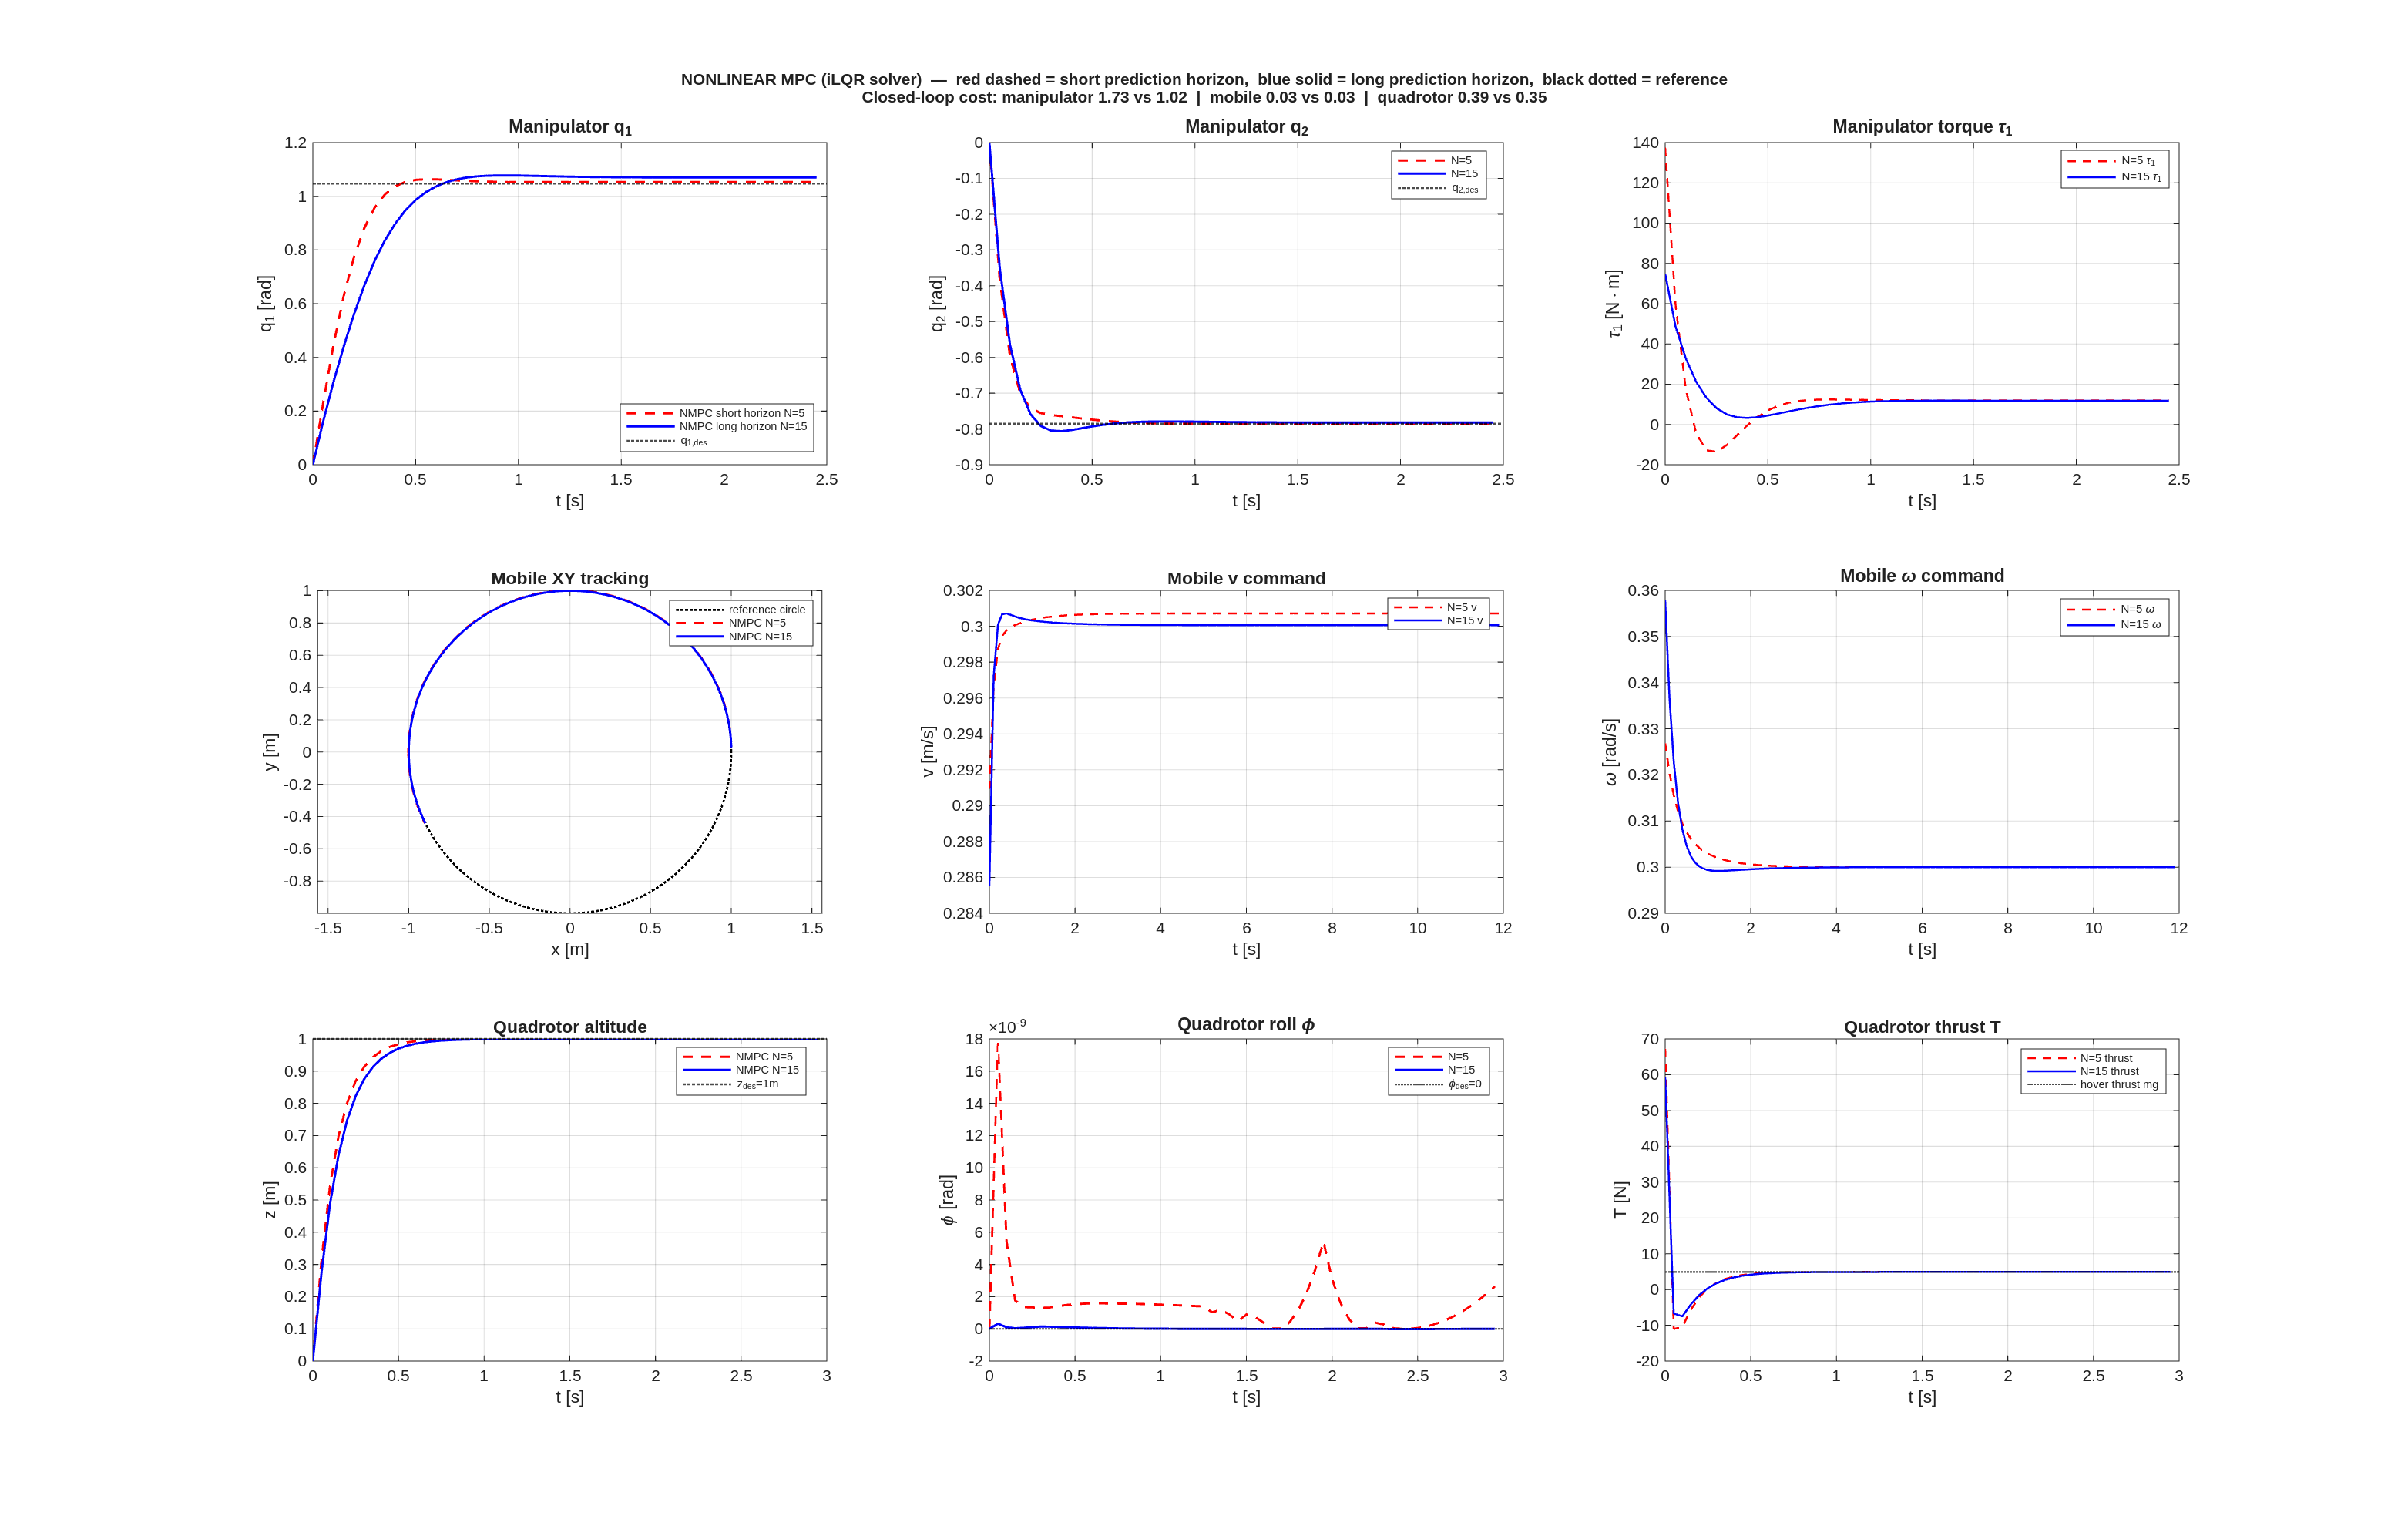
\includegraphics[width=0.85\textwidth]{images/week_08/nmpc_results.png}

Figure 9.1 --- NMPC with short (\textbackslash(N\textbackslash!=\textbackslash!5\textbackslash), red dashed) vs. long (\textbackslash(N\textbackslash!=\textbackslash!15\textbackslash), blue solid) prediction horizon on all three robots. Longer horizon consistently improves or matches the shorter one.

\begin{longtable}[]{@{}lllll@{}}
\toprule\noalign{}
Robot & State dim. & \textbackslash(N\_\{\textbackslash text\{short\}\}\textbackslash) / \textbackslash(J\_\{cl\}\textbackslash) & \textbackslash(N\_\{\textbackslash text\{long\}\}\textbackslash) / \textbackslash(J\_\{cl\}\textbackslash) & Horizon benefit \\
\midrule\noalign{}
\endhead
\bottomrule\noalign{}
\endlastfoot
Manipulator (regulation) & 4 & 5 / 1.730 & 15 / 1.020 & −41.0\% \\
Mobile robot (circle tracking) & 3 & 5 / 0.0313 & 15 / 0.0315 & saturated (both near-perfect) \\
Quadrotor (altitude + attitude) & 6 & 5 / 0.393 & 15 / 0.346 & −12.0\% \\
\end{longtable}

\textbf{Why iLQR works where simplex methods fail:} a 2N-dimensional NLP solved by Nelder-Mead simplex needs \textbackslash(O(10\^{}3)\textbackslash) iterations per sample and still rarely converges. iLQR exploits the \emph{causal structure} of the shooting problem --- one Gauss-Newton step touches every control variable via a single backward sweep --- giving quadratic local convergence in \textbackslash(O(10)\textbackslash) outer iterations.

\textbf{The real-time constraint.} The mobile result is saturated because the unicycle has a 3-state, 2-input model and the circle is easy to track --- horizon 5 is already more than enough. The manipulator and quadrotor both benefit from the longer horizon, as expected for higher-dimensional problems. In deployment, you would profile \texttt{tic/toc} around the solver and shrink the horizon to the shortest value that keeps the stability certificate.

\subsection{Section 10: Unified View --- Every Nonlinear Controller as an Optimization Problem}\label{section-10-unified-view-every-nonlinear-controller-as-an-optimization-problem}}

\subsubsection{10.1 The common template}\label{the-common-template}}

Every controller we have studied fits the pattern:

controller = stability certificate (Lyapunov / CLF / s=0) + free parameters \textbackslash(\textbackslash theta\textbackslash) + performance objective \textbackslash(J(\textbackslash theta)\textbackslash)

Optimization chooses \textbackslash(\textbackslash theta\textbackslash) to minimize \textbackslash(J\textbackslash) subject to the certificate remaining valid.

\subsubsection{10.2 Master summary table}\label{master-summary-table}}

\begin{longtable}[]{@{}lllll@{}}
\toprule\noalign{}
Controller & Decision variables & Cost function & Constraints & Typical solver \\
\midrule\noalign{}
\endhead
\bottomrule\noalign{}
\endlastfoot
Sliding Mode & \textbackslash(\textbackslash lambda,\textbackslash phi,\textbackslash eta\textbackslash) & tracking + effort + chatter & \textbackslash(\textbackslash eta \textgreater{} D\textbackslash), \textbackslash(\textbackslash phi\textgreater0\textbackslash) & fminsearch / BayesOpt / LMI for surface \\
Adaptive (MRAC) & \textbackslash(\textbackslash Gamma,\textbackslash sigma\textbackslash), projection bounds & tracking + effort & \textbackslash(\textbackslash Gamma\textbackslash succ 0,\textbackslash{} \textbackslash sigma\textbackslash geq 0\textbackslash), physical bounds on \textbackslash(\textbackslash hat\textbackslash theta\textbackslash) & fminsearch / BayesOpt \\
Robust (\textbackslash(H\_\textbackslash infty\textbackslash)) & weighting filters \textbackslash(W\_S,W\_T,W\_\{KS\}\textbackslash); or polytopic \textbackslash(K\textbackslash) & \textbackslash(H\_\textbackslash infty\textbackslash) norm of weighted sensitivity & closed-loop stability & hinfsyn / DK-iteration / LMI \\
Backstepping & \textbackslash(k\_1,\textbackslash ldots,k\_n\textbackslash); command-filter BW \textbackslash(\textbackslash omega\_f\textbackslash) & tracking + effort + smoothness & \textbackslash(k\_i\textgreater0\textbackslash), CLF \textbackslash(\textbackslash dot V\_n\textless0\textbackslash) & fminsearch / Bayesian optimization \\
NMPC & \textbackslash(N,Q,R,P,\textbackslash mathcal X\_f,\textbackslash Delta t\textbackslash) & closed-loop integrated cost + solve-time & recursive feasibility, terminal invariance & SQP/IPM + offline LQR for \textbackslash((P,\textbackslash mathcal X\_f)\textbackslash) \\
iLQR / DDP (open-loop) & trajectory \textbackslash(\textbackslash\{u\_k\textbackslash\}\_\{k=0\}\^{}\{N-1\}\textbackslash) & tracking + effort + terminal & dynamics, \textbackslash(u\textbackslash in\textbackslash mathcal U\textbackslash) & iLQR / DDP Newton iterations \\
\end{longtable}

\subsubsection{10.3 Cross-cutting optimization tools}\label{cross-cutting-optimization-tools}}

\paragraph{LMIs \& SDP}\label{lmis-sdp}}

Convex, globally optimal for any Lyapunov-based design that can be posed as an LMI (robust state-feedback, SMC surface, ISS gain).

\paragraph{SOS programming}\label{sos-programming}}

Certifies polynomial Lyapunov functions --- needed for non-quadratic certificates. Backend: SDP.

\paragraph{Bayesian optimization}\label{bayesian-optimization}}

Sample-efficient tuning for black-box controllers on hardware. Minimizes physical trial count when each experiment is expensive.

\paragraph{Reinforcement learning}\label{reinforcement-learning}}

Policy-gradient on a parameterized controller \textbackslash(\textbackslash pi\_\textbackslash theta\textbackslash) --- subsumes all of the above when the reward encodes the cost. Stability not free.

\paragraph{Differentiable simulation}\label{differentiable-simulation}}

Compute \textbackslash(\textbackslash nabla\_\textbackslash theta J\textbackslash) directly through the simulator (autodiff). Gives gradient-based methods the power of BayesOpt at much lower sample cost.

\paragraph{Scenario / stochastic programming}\label{scenario-stochastic-programming}}

Optimizes over a distribution of uncertain parameters rather than a worst case --- average-case robust design.

\subsection{Section 11: MATLAB Lab Activities}\label{section-11-matlab-lab-activities}}

\subsubsection{Setup}\label{setup-3}}

All simulations live in \texttt{week\_08/sims/} and run on base MATLAB (no toolboxes beyond Control System Toolbox required). They use \texttt{fminsearch} for the parameter optimization and explicit Euler or \texttt{ode}-style integration for the dynamics.

\% From MATLAB, cd to the lab directory
cd /home/it-services/auto\_control\_ws/week\_08/sims
\% Run everything (\textasciitilde30 s on a modern laptop)
run\_all
\% Or run a single controller
sim\_smc \% sliding mode
sim\_adaptive \% adaptive / MRAC
sim\_robust \% robust min-max
sim\_backstepping \% backstepping
sim\_nmpc \% nonlinear MPC

\subsubsection{Activity 1 --- SMC Pareto sweep (15 min)}\label{activity-1-smc-pareto-sweep-15-min}}

Inside \texttt{sim\_smc.m}, change the cost weights \textbackslash((w\_e, w\_u, w\_c)\textbackslash) on the chatter term. Re-run and observe:

\begin{itemize}
\tightlist
\item
  Small \textbackslash(w\_c\textbackslash): optimizer picks a \emph{narrow} boundary layer (low \textbackslash(\textbackslash phi\textbackslash)) --- sharp tracking, chattering control
\item
  Large \textbackslash(w\_c\textbackslash): optimizer picks a \emph{wide} boundary layer --- smooth torque, residual tracking error
\end{itemize}

\textbf{Deliverable:} plot the Pareto front of tracking error vs. chatter metric across \textbackslash(w\_c \textbackslash in \textbackslash\{0.001, 0.01, 0.1, 1\textbackslash\}\textbackslash).

\subsubsection{\texorpdfstring{Activity 2 --- Adaptive optimizer tells you when \emph{not} to adapt (10 min)}{Activity 2 --- Adaptive optimizer tells you when not to adapt (10 min)}}\label{activity-2-adaptive-optimizer-tells-you-when-not-to-adapt-10-min}}

Set the payload disturbance to zero in \texttt{sim\_adaptive.m} (make \texttt{p\_true\ =\ p}). Re-run and inspect the optimized \textbackslash(\textbackslash Gamma\textbackslash). Discuss: why does the optimizer drive \textbackslash(\textbackslash Gamma\textbackslash to 0\textbackslash)?

\subsubsection{Activity 3 --- Robust vs. average-case (15 min)}\label{activity-3-robust-vs.-average-case-15-min}}

Modify \texttt{robust\_quad\_cost} to use the \emph{mean} rather than \emph{max} over the uncertainty set. Compare the resulting gains. Under which uncertainty distribution is the average-case design acceptable, and when does the worst-case matter?

\subsubsection{Activity 4 --- NMPC horizon sweep (15 min)}\label{activity-4-nmpc-horizon-sweep-15-min}}

Run \texttt{sim\_nmpc} with the horizon set to \textbackslash(N = \textbackslash\{3,5,7,10,15,25\textbackslash\}\textbackslash) on the quadrotor. Record closed-loop cost \emph{and} per-step solve time (\texttt{tic/toc} around the \texttt{fminsearch} call). Plot both on one graph. Identify the knee of the curve --- this is your deployment horizon.

\textbf{Last run on this machine (R2025b):} total wall time \textasciitilde43~s for all five controllers on all three robots (iLQR-based NMPC dominates the wall-clock). Cost reductions ranged from 2\% (manipulator robust --- already near worst-case optimum) to 88\% (mobile backstepping); NMPC manipulator benefited by 41\% from extending the horizon.

\subsection{Appendix: Week 7 Recall --- Sliding Mode Control (Exam Practice)}\label{appendix-week-7-recall-sliding-mode-control-exam-practice}}

\paragraph{Question 1 --- SMC Controller Design and Stability Proof (25 marks)}\label{question-1-smc-controller-design-and-stability-proof-25-marks}}

Consider a robot manipulator governed by:

\textbackslash{[}
M(q)\textbackslash ddot\{q\} + C(q,\textbackslash dot\{q\})\textbackslash dot\{q\} + G(q) = \textbackslash tau + d(t)
\textbackslash{]}

where \textbackslash(d(t)\textbackslash) represents matched uncertainty with known bound \textbackslash(\textbackslash\textbar d(t)\textbackslash\textbar{} \textbackslash leq D\textbackslash).

\textbf{(a)} Define the tracking error \textbackslash(e = q - q\_d\textbackslash) and the sliding surface:

\textbackslash{[} s = \textbackslash dot\{e\} + \textbackslash Lambda e \textbackslash{]}

where \textbackslash(\textbackslash Lambda = \textbackslash text\{diag\}(\textbackslash lambda\_1, \textbackslash ldots, \textbackslash lambda\_n)\textbackslash) with \textbackslash(\textbackslash lambda\_i \textgreater{} 0\textbackslash). Explain why the system trajectories converge to \textbackslash(e = 0\textbackslash) exponentially once \textbackslash(s = 0\textbackslash).

\paragraph{Model Answer (a)}\label{model-answer-a}}

When \textbackslash(s = 0\textbackslash), \textbackslash(\textbackslash dot e = -\textbackslash Lambda e\textbackslash); with all \textbackslash(\textbackslash lambda\_i\textgreater0\textbackslash), \textbackslash(e(t)=e(0)e\^{}\{-\textbackslash Lambda t\}\textbackslash) converges exponentially with time constants \textbackslash(1/\textbackslash lambda\_i\textbackslash).

\textbf{(b)} Derive the equivalent control \textbackslash(\textbackslash tau\_\{eq\}\textbackslash) by setting \textbackslash(\textbackslash dot\{s\} = 0\textbackslash) (assuming \textbackslash(d = 0\textbackslash)).

\paragraph{Model Answer (b)}\label{model-answer-b}}

\textbackslash{[} \textbackslash boxed\{\textbackslash tau\_\{eq\} = M(q)\textbackslash bigl(\textbackslash ddot\{q\}\_d - \textbackslash Lambda\textbackslash dot\{e\}\textbackslash bigr) + C(q,\textbackslash dot\{q\})\textbackslash dot\{q\} + G(q)\} \textbackslash{]}

\textbf{(c)} With switching term \textbackslash(\textbackslash tau\_\{sw\} = -K\textbackslash,\textbackslash text\{sign\}(s)\textbackslash) and Lyapunov function \textbackslash(V = \textbackslash tfrac\{1\}\{2\}s\^{}\{T\}M(q)s\textbackslash), show \textbackslash(\textbackslash dot V \textbackslash leq -(k\_\{\textbackslash min\}-D)\textbackslash\textbar s\textbackslash\textbar\_1\textbackslash) when \textbackslash(k\_i \textgreater{} D\textbackslash).

\paragraph{Model Answer (c)}\label{model-answer-c}}

Using skew-symmetry of \textbackslash(\textbackslash dot M - 2C\textbackslash): \textbackslash(\textbackslash dot V = s\^{}\{T\}(M\textbackslash dot s + Cs) = s\^{}\{T\}(\textbackslash tau\_\{sw\}+d) = -\textbackslash sum k\_i\textbar s\_i\textbar{} + s\^{}\{T\}d \textbackslash leq -(k\_\{\textbackslash min\}-D)\textbackslash\textbar s\textbackslash\textbar\_1\textbackslash). \textbackslash(\textbackslash square\textbackslash)

\paragraph{Question 2 --- Chattering \& boundary layer (20 marks)}\label{question-2-chattering-boundary-layer-20-marks}}

(a) Explain chattering and why it harms actuators. (b) Derive the steady-state error bound \textbackslash(\textbar e\_\{ss\}\textbar{} \textbackslash leq \textbackslash phi/\textbackslash lambda\textbackslash) for boundary-layer SMC.

\paragraph{Model Answer (condensed)}\label{model-answer-condensed}}

Chattering comes from the discontinuous \textbackslash(\textbackslash text\{sign\}(s)\textbackslash) combined with sampling / unmodelled dynamics. Replacing by \textbackslash(\textbackslash mathrm\{sat\}(s/\textbackslash phi)\textbackslash) yields a high-gain proportional law inside the layer; in steady state \textbackslash(\textbar s\textbar\textbackslash leq \textbackslash phi D/k\textbackslash), and since \textbackslash(s=\textbackslash dot e+\textbackslash lambda e\textbackslash) the tracking-error bound is \textbackslash(\textbar e\_\{ss\}\textbar\textbackslash leq \textbackslash phi/\textbackslash lambda\textbackslash).

\subsection{Section 13: Course Recap \& What\textquotesingle s Next}\label{section-13-course-recap-whats-next}}

\subsubsection{13.1 The nonlinear control theory journey}\label{the-nonlinear-control-theory-journey}}

\paragraph{Weeks 1--3: MPC}\label{weeks-13-mpc}}

Prediction + optimization. Set the stage for NMPC.

\paragraph{Week 4: Adaptive}\label{week-4-adaptive}}

Online parameter learning with Lyapunov certificates.

\paragraph{Week 5: Robust}\label{week-5-robust}}

Fixed controller for worst-case plant.

\paragraph{Week 6: Backstepping}\label{week-6-backstepping}}

Recursive CLF design for strict-feedback systems.

\paragraph{Week 7: SMC}\label{week-7-smc}}

Variable structure, discontinuous robustness.

\paragraph{Week 8 (this): Optimization of all of the above}\label{week-8-this-optimization-of-all-of-the-above}}

Every controller has free parameters; every choice of parameters is an optimization.

\subsubsection{13.2 Unifying themes}\label{unifying-themes}}

\begin{itemize}
\tightlist
\item
  \textbf{Nonlinearity is the defining feature of robots} --- we never linearized at design time in this course.
\item
  \textbf{Lyapunov certificates give the feasible set} of the parameter optimization --- any \textbackslash(\textbackslash theta\textbackslash) that breaks the certificate is excluded.
\item
  \textbf{Optimization is how we pick good controllers, not just good trajectories} --- Section 3.3\textquotesingle s (A) vs (B) distinction.
\item
  \textbf{Compute is a first-class constraint} --- NMPC and adaptive tuning are only useful at real-time sample rates.
\end{itemize}

\subsubsection{13.3 What\textquotesingle s next --- Automation block}\label{whats-next-automation-block}}

Weeks 9--12 shift from control theory to deployment: state machines, ROS 2 integration, perception, and system-level projects. The tuned controllers from this week become the low-level primitives those higher-level systems will invoke.

\textbf{Control for Robots --- M.Sc. Programme}

University of West London • AY 2025--26

Week 8: Nonlinear Control Optimization for Robotic Systems
